 % Don't put any content in here. 
 % Don't even include content files by using \input or \inlcude. 
 % Put your content to TEXT.TEX or include it there using \input.
 % Uses:
 %		SETTINGS.TEX	contains the settings for this document
 %		COMMANDS.TEX	contains commands which can be used while writing
 %		INFO.TEX			contains the author, title and so on for the cover
 %		COVER.TEX			formats the front cover of the document
 %		ABSTRACT.TEX	contains the abstract to be included (if needed)
 %		TEXT.TEX			contains the actual content of the document
 %		BIB.BIB				containt the BibTeX entries for the document
 
 


\documentclass[11pt,a4paper,bibtotoc,idxtotoc,headsepline,footsepline,footexclude,BCOR12mm,DIV13]{scrbook}


% KOMA-Optionen:
%  bibtotoc: include bibliography in table of contents
%  idxtotoc: include index in table of contents
%  headsepline: use horizontalline under heading
%  BCOR: binding correcion (Bindungskorrektur) (e.g.: BCOR5mm)
%  DIV: Number of sheet sections (used for layout) (e.g.: DIV12) 



% include title and author information for the cover
% Set here the title, authors and other stuff to be used for the cover
% This file is used by MAIN.TEX

% set title, authors and stuff for the cover
\def\doctype{Master's Thesis in Informatics}
\def\title{Evaluation and Prediction of Execution Times for OpenCL-based Computations on GPGPU Systems}
\def\titleGer{Evaluierung und Vorhersage von Ausf\"uhrungszeiten f\"ur OpenCL-basierte Berechnungen auf GPGPU-Systemen}
\def\author{Alexander P\"oppl}
\def\date{August 15th, 2014}

% text to appear in the footer
\def\footertext{}

% include settings
% Included by MAIN.TEX
% Defines the settings for the CAMP report document

\renewcommand{\sectfont}{\normalfont \bfseries}        % Schriftart der Kopfzeile

% manipulate footer
\usepackage{scrpage2}
\pagestyle{scrheadings}
\ifoot[\footertext]{\footertext} % \footertext set in INFO.TEX
%\setkomafont{pagehead}{\normalfont\rmfamily}
\setkomafont{pagenumber}{\normalfont\rmfamily}

%% allow sophisticated control structures
\usepackage{ifthen}

% use Palatino as default font
\usepackage{palatino}

% enable special PostScript fonts
\usepackage{pifont}

%to use the subfigures
\usepackage{subcaption}


\usepackage{colortbl}

% Double Spacing for Review.
%\usepackage[doublespacing]{setspace}

%% enable TUM symbols on title page
\usepackage{styles/tumlogo}

\usepackage{multirow}

%% use colors
\usepackage{color}

%% make fancy math
\usepackage{amsmath}
\usepackage{amsfonts}
\usepackage{amssymb}
\usepackage{stmaryrd}
\usepackage{textcomp}
\usepackage{yhmath} % for the adots 


%% create an index
\usepackage{makeidx}

% for the program environment
\usepackage{float}

%% load german babel package for german abstract
%\usepackage[german,american]{babel}
\usepackage[german,english]{babel}
\selectlanguage{english}

% use german characters as well
\usepackage[utf8]{inputenc}       % allow utf8 characters

% TikZ, PGF and such
% UML diagrams
\usepackage{pgf}
\usepackage{tikz}
\usepackage{styles/pgf-umlcd}
\usepackage{pgfplots, pgfplotstable}
\pgfplotsset{compat=1.8}
\usepgfplotslibrary{statistics}
\usetikzlibrary{arrows,automata,shapes.geometric}
\tikzstyle{startstop} = [rectangle, rounded corners, minimum width=3cm, minimum height=1cm,text centered, draw=black, fill=red!30]
\tikzstyle{io} = [trapezium, trapezium left angle=70, trapezium right angle=110, minimum width=3cm, minimum height=1cm, text centered, draw=black, fill=blue!30]
\tikzstyle{process} = [rectangle, minimum width=3cm, minimum height=1cm, text centered, draw=black, fill=orange!30]
\tikzstyle{decision} = [diamond, minimum width=3cm, minimum height=1cm, text centered, draw=black, fill=green!30]
\tikzstyle{arrow} = [thick,->,>=stealth]


\usepackage{listings}

%\usepackage{styles/shortoverview}
%----------------------------------------------------
%      Graphics and Hyperlinks
%----------------------------------------------------

%% check for pdfTeX
\ifx\pdftexversion\undefined
 %% use PostScript graphics
 \usepackage[dvips]{graphicx}
 \DeclareGraphicsExtensions{.eps,.epsi}
 \graphicspath{{figures/}{figures/review}} 
 %% allow rotations
 \usepackage{rotating}
 %% mark pages as draft copies
 %\usepackage[english,all,light]{draftcopy}
 %% use hypertex version of hyperref
 \usepackage[hypertex,hyperindex=false,colorlinks=false]{hyperref}
\else %% reduce output size \pdfcompresslevel=9
 %% declare pdfinfo
 %\pdfinfo { 
 %  /Title (my title) 
 %  /Creator (pdfLaTeX) 
 %  /Author (my name) 
 %  /Subject (my subject	) 
 %  /Keywords (my keywords)
 %}
 %% use pdf or jpg graphics
 %\usepackage[pdftex]{graphicx}
 %\DeclareGraphicsExtensions{.jpg,.JPG,.png,.pdf,.eps}
 %\graphicspath{{figures/}} 
 
 %% Load float package, for enabling floating extensions
 \usepackage{float}
 
 %% allow rotations
 \usepackage{rotating}
 %% use pdftex version of hyperref
 \usepackage[pdftex,colorlinks=true,linkcolor=blue,citecolor=blue,%
 anchorcolor=blue,urlcolor=blue,bookmarks=true,%
 bookmarksopen=true,bookmarksopenlevel=0,plainpages=false,%
 bookmarksnumbered=true,hyperindex=false,pdfstartview=%
 ]{hyperref}
 \usepackage[nomain,acronym,xindy,toc]{glossaries}
 \makeglossaries

%\usepackage[pdftex,colorlinks=false,linkcolor=red,citecolor=red,%
% anchorcolor=red,urlcolor=red,bookmarks=true,%
% bookmarksopen=true,bookmarksopenlevel=0,plainpages=false%
% bookmarksnumbered=true,hyperindex=false,pdfstartview=%
% ]{hyperref}
\fi




%% Fancy chapters
%\usepackage[Lenny]{fncychap}
%\usepackage[Glenn]{fncychap}
%\usepackage[Bjarne‚]{fncychap}

%\usepackage[avantgarde]{quotchap}

% set the bibliography style
%\bibliographystyle{styles/bauermaNum}
%\bibliographystyle{alpha}
\bibliographystyle{plain}

% include commands
% Commands to be used within the TUM report document
% Included by MAIN.TEX
% Please include your own cool commands here. 
% Be only sure to comment it sufficiently so others can use it.

%-------------------------------------------------------------
%                      Own Commands
%-------------------------------------------------------------


%-------------------------------------------------------------
% math stuff -------------------------------------------------

% nice R, N, C
\newcommand{\nat}{\mathbb{N}}
\newcommand{\real}{\mathbb{R}}
\newcommand{\compl}{\mathbb{C}}



% norm
\newcommand{\norm}[1]{\left\| #1 \right\|}

% un demi
\newcommand{\half}{\frac{1}{2}}

% parantheses
\newcommand{\parenth}[1]{ \left( #1 \right) }
\newcommand{\bracket}[1]{ \left[ #1 \right] }
\newcommand{\accolade}[1]{ \left\{ #1 \right\} }
\newcommand{\abstsyntax}[1]{\llbracket #1 \rrbracket^\sharp}

%\newcommand{\angle}[1]{ \left\langle  #1 \right\rangle }

% partial derivative: %#1 function, #2 which variable
% simple / single line version
\newcommand{\pardevS}[2]{ \delta_{#1} f(#2) }
% fraction version
\newcommand{\pardevF}[2]{ \frac{\partial #1}{\partial #2} }

% render vectors: 3 and 4 dimensional
\newcommand{\veciii}[3]{\left[ \begin{array}[h]{c} #1 \\ #2 \\ #3	\end{array} \right]}
\newcommand{\veciv}[4]{\left[ \begin{array}[h]{c} #1 \\ #2 \\ #3 \\ #4	\end{array} \right]}

% render matrices: 3  dimensional (arguments in row first order)
\newcommand{\matiii}[9]{\left[ \begin{array}[h]{ccc} #1 & #2 & #3 \\ #4 & #5 & #6 \\ #7 & #8 & #9	\end{array} \right]}
%DOESN'T WORK,DON'T KNOW WHY \newcommand{\mativ}[16]{\left[ \begin{array}[h]{cccc} #1 & #2 & #3 & #4 \\ #5 & #6 & #7 & #8 \\ #9 & #10 & #11 & #12 \\ #13 & #14 & #15 & #16 \end{array} \right]}


%-------------------------------------------------------------
%-------------------------------------------------------------


%-------------------------------------------------------------
% some abreviations ------------------------------------------
\newcommand{\Reg}{$^{\textregistered}$}
\newcommand{\reg}{$^{\textregistered}$ }
\newcommand{\Tm}{\texttrademark}
\newcommand{\tm}{\texttrademark~}
\newcommand {\bsl} {$\backslash$}
%-------------------------------------------------------------
%------------------------------------------------------------- 


%-------------------------------------------------------------
% some custom operators --------------------------------------
\DeclareMathOperator{\Node}{Node}
\DeclareMathOperator{\Leaf}{Leaf}
\DeclareMathOperator{\Path}{Path}


%-------------------------------------------------------------
%------------------------------------------------------------- 


%-------------------------------------------------------------
% formating --------------------------------------------------

% Theorem & Co environments and counters
\newtheorem{theorem}{Theorem}[chapter]
\newtheorem{lemma}[theorem]{Lemma}
\newtheorem{corollary}[theorem]{Corollary}
\newtheorem{remark}[theorem]{Remark}
\newtheorem{definition}[theorem]{Definition}
\newtheorem{equat}[theorem]{Equation}
\newtheorem{example}[theorem]{Example}
\newtheorem{algorithm}[theorem]{Algorithm}

% inserting figures
\newcommand{\insertfigure}[4]{ % Filename, Caption, Label, Width percent of textwidth
	\begin{figure}[htbp]
		\begin{center}
			\includegraphics[width=#4\textwidth]{#1}
		\end{center}
		\vspace{-0.4cm}
		\caption{#2}
		\label{#3}
	\end{figure}
}




% referecing figures

\newcommand{\refFigure}[1]{ %label
	figure \ref{#1}
}
\newcommand{\refChapter}[1]{ %label
	chapter \ref{#1}
}

\newcommand{\refSection}[1]{ %label
	section \ref{#1}
}

\newcommand{\refParagraph}[1]{ %label
	paragraph \ref{#1}
}

\newcommand{\refEquation}[1]{ %label
	equation \ref{#1}
}

\newcommand{\refTable}[1]{ %label
	table \ref{#1}
}




\newcommand{\rigidTransform}[2]
{
	${}^{#2}\!\mathbf{H}_{#1}$
}

%code, in typewriter
\newcommand{\code}[1]
 {\texttt{#1}}

% comment that appears on the border - very practical !!!
\newcommand{\comment}[1]{\marginpar{\raggedright \noindent \footnotesize {\sl #1} }}

% page clearing
\newcommand{\clearemptydoublepage}{%
  \ifthenelse{\boolean{@twoside}}{\newpage{\pagestyle{empty}\cleardoublepage}}%
  {\clearpage}}


%-------------------------------------------------------------
%-------------------------------------------------------------


\newcommand{\etAl}{\emph{et al.}\mbox{ }}


%\makeindex
	%% inter line spacing
%\linespread{1.0}

\makeglossary

\begin{document}
	\newglossaryentry{OpenCL}
 {
   name=OpenCL,
   description={is a programmable machine that receives input,
                stores and manipulates data, and provides
                output in a useful format}
}
	\frontmatter	
	% The front cover for the TUM report document.
% Included by MAIN.TEX


%--------------------------------------------------
% The Front Cover
%--------------------------------------------------

% The front cover for the TUM document.
% Included by MAIN.TEX


%--------------------------------------------------
% The Front Cover
%--------------------------------------------------

% correct BCOR - undo at the end !!!
\def\bcorcor{0.15cm}
\addtolength{\hoffset}{\bcorcor}

\thispagestyle{empty}

 \vspace{4cm}
\begin{center}
	       \oTUM{4cm}
	   
	   \vspace{5mm}     
%	   \huge FAKULT{\"A}T F{\"U}R INFORMATIK\\ 
     \huge DEPARTMENT OF INFORMATICS\\
	   \vspace{0.5cm}
	 \large TECHNISCHE UNIVERSIT{\"A}T M{\"U}NCHEN\\
    \vspace{1mm}
        
	\end{center}
		

\vspace{15mm}
\begin{center}

   {\Large \doctype}

  \vspace{20mm}
  
  {\huge\bf \title}\\%[3ex]
  
  
  \vspace{15mm}
  
  
  {\LARGE  \author}
  
  \vspace{10mm}
  
  \begin{figure}[h!]
  \centering
   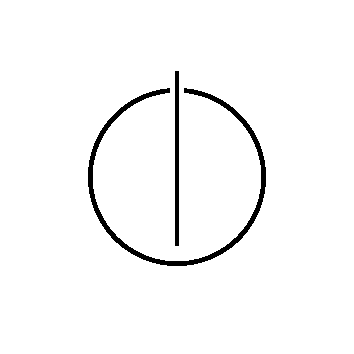
\includegraphics[width=4cm]{styles/informat.png}
  \end{figure}
  
  \end{center}
	\clearemptydoublepage
	% The titlepage for the CAMP report document.
% Included by MAIN.TEX


%--------------------------------------------------
% The title page
%--------------------------------------------------

% correct BCOR - undo at the end !!!
\def\bcorcor{0.15cm}
\addtolength{\hoffset}{\bcorcor}

\thispagestyle{empty}

 \vspace{10mm}
\begin{center}
	       \oTUM{4cm}
	   
	   \vspace{5mm}     
%	   \huge FAKULT{\"A}T F{\"U}R INFORMATIK\\ 
	   \huge DEPARTMENT OF INFORMATICS\\
	   \vspace{0.5cm}
	 \large TECHNISCHE UNIVERSIT{\"A}T M{\"U}NCHEN\\
        
	\end{center}
		

\vspace{10mm}
\begin{center}

   {\Large \doctype}

  \vspace{10mm}
  
  {\LARGE \title}\\
  
  
  \vspace{10mm}
  
  
  {\LARGE  \titleGer}\\
  
  
  \vspace{10mm}

    %\hfill
    \begin{tabular}{ll}
	   \Large Author:     & \Large \author \\[2mm]
	   \Large Supervisor:    & \Large Prof. Dr. Helmut Seidl \\[2mm]				
	   \Large Advisor:	& \Large Dipl. Phys. Alexander Herz\\[2mm]
	   \Large Date:       & \Large \date
	 \end{tabular}
	 
	 \vspace{5mm}
	 
	 \begin{figure}[h!]
  \centering
   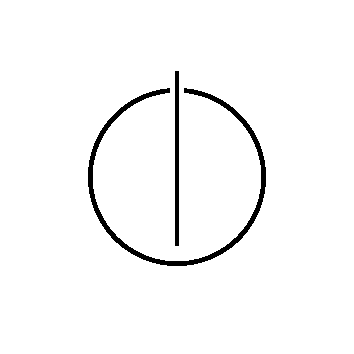
\includegraphics[width=4cm]{styles/informat.png}
  \end{figure}
   

\end{center}

% undo BCOR correction
\addtolength{\hoffset}{\bcorcor}
	\clearemptydoublepage


\thispagestyle{empty}
\selectlanguage{german}
	\vspace*{0.75\textheight}
	\noindent
	Ich versichere, dass ich diese Master's Thesis selbst{\"a}ndig verfasst und nur 
	die angegebenen Quellen und Hilfsmittel verwendet habe.
	
	\vspace{5mm}
	\noindent
	I confirm that this master's thesis is my own work and I have documented all sources and material used.
	
	\vspace{20mm}
	\noindent
	M{\"u}nchen, den \today \hspace{5cm} \author
\selectlanguage{english}
\newpage
	\clearemptydoublepage
\phantomsection
\addcontentsline{toc}{chapter}{Acknowledgements}	


%\chapter*{Acknowledgements}

\vspace*{2cm}

\begin{center}
{\Large \bf Acknowledgments}
\end{center}

\vspace{1cm}




I'd like to thank everyone for the support given to me whilst writing this thesis. Thank you Neil for correcting my English. Thank you to all the people I talked to about my ideas. Thank you everyone who helped me in little ways.
	% Abstract for the TUM report document
% Included by MAIN.TEX


\clearemptydoublepage
\phantomsection
\addcontentsline{toc}{chapter}{Abstract}	





\vspace*{2cm}
\begin{center}
{\Large \bf Abstract}
\end{center}
\vspace{1cm}

This thesis presents a run time prediction model for domain iterations on GPUs. The model includes predictions about transferring data to and from the compute device, the influence of the size of the work-group and kernel base costs. On top of that, a cost model is established for basic operations and memory accesses, taking into account effects of having multiple basic operations or memory accesses in one kernel, and the properties of different kinds of memory access classes. The thesis also describes the benchmark suite developed to take the measurements the model is based on. It also explains the additions made to the funkyIMP compiler in order to facilitate the execution of code on the GPU. The thesis concludes by giving an evaluation of the predictions made with the help of the model. \\

In dieser Arbeit wird eine Modell zur Vorhersage von Ausführungszeiten für Domain Iterations auf GPUs präsentiert. Dieses Modell beinhaltet Vorhersagen über den Transfer von Daten zu und von der Grafikkarte, den Einfluss der Größe der Work-Group, und den Grundkosten bei der Ausführung von Kernels auf der GPU. Dazu wird ein Kostenmodell für Rechenoperationen und Speicherzugriffe etabliert, das auch die Effekte von mehreren Rechenoperationen oder Speicherzugriffen innerhalb eines Kernels berücksichtigt. Außerdem werden Speicherzugriffe in verschiedene Klassen eingeteilt und separat bewertet. In der Arbeit wird auch die Benchmark Suite beschrieben, die im Laufe der Masterarbeit entstanden ist, um die Messungen die dem Modell zu Grunde liegen vorzunehmen. Weiterhin werden die Erweiterungen beschrieben, die am funkyIMP Compiler vorgenommen wurden, um die Ausführung von Code auf der GPU zu ermöglichen. Abschließend wird eine Bewertung der Vorhersagen, die mit dem Modell erstellt wurden durchgeführt.
	\tableofcontents
  	\clearemptydoublepage

\phantomsection
\addcontentsline{toc}{chapter}{Outline of the Thesis}

\begin{center}
	\huge{Outline of the Thesis}
\end{center}




%--------------------------------------------------------------------
\section*{Part I: Introduction and Theory}

\noindent {\scshape Chapter 1: Introduction}  \vspace{1mm}

\noindent  This chapter presents a general introduction and motivation to the topic of parallel and general purpose GPU computing.\\

\noindent {\scshape Chapter 2: Theory}  \vspace{1mm}

\noindent  This chapter introduces the relevant technologies that are used in the implementation, namely OpenCL and FunkyIMP.   \\

%--------------------------------------------------------------------
\section*{Part II: Methodology}

\noindent {\scshape Chapter 3: Extensions to the funkyIMP Compiler}  \vspace{1mm}

\noindent  This chapter presents the extensions that were made to the funkyIMP compiler in order to accommodate the automated compilation of code on the GPU.   \\

\noindent {\scshape Chapter 4: The Benchmark Suite}  \vspace{1mm}

\noindent  This chapter presents the benchmark suite that was written to create a model of the runtime of the individual operations in OpenCL.   \\

%--------------------------------------------------------------------
\section*{Part III: Runtime Model and Results}

\noindent {\scshape Chapter 5: A Runtime Prediction Model}  \vspace{1mm}

\noindent  This chapter introduces presents the actual runtime model for OpenCL operations.   \\

\noindent {\scshape Chapter 6: Results and Evaluation}  \vspace{1mm}

\noindent  In this chapter, the results achieved in the course of this thesis are shown. The quality of the predictions made utilizing the runtime prediction model is evaluated on a quantitative scale.\\

%--------------------------------------------------------------------
\section*{Part IV: Further Work and Conclusion}

\noindent {\scshape Chapter 7: Future Work}  \vspace{1mm}

\noindent  There are topics that did not fit in the scope of this thesis. This chapter discusses several of these.   \\

\noindent {\scshape Chapter 8: Conclusion}  \vspace{1mm}

\noindent  In this chapter the results of this thesis are evaluated on a qualitative scale.  \\
	\mainmatter
	% Included by MAIN.TEX
% Put your content in here or include it by using \input (\include won't work)

\addtolength{\evensidemargin}{-12mm}

% ---------------------------------------------------------------------------
%
%Introduction and Background Theory
%
% ---------------------------------------------------------------------------
\part[Introduction and Theory]{Introduction and Theory}
\label{part:introAndTheory}
% !TEX root = ../main.tex

\chapter{Introduction}
\label{chap:intro}
After a period of incredible advances in processing power in the Eighties, Nineties and early 2000s, progress in the field of classical single core CPUs has slowed considerably in the last 10 years. Given the ever increasing complexity of modern computer programs, different solutions had to be found. Once single core performance could not be increased at a sufficient speed anymore, the tendency to execute code in parallel arose instead. For example, modern CPUs usually have at least two cores, a lot of them even four or more. This trend is no longer specific to traditional computers such as PCs and servers, but can also be found on mobile devices such as smart phones and tablets. \\

There are two different ways to parallelize applications, i.e. task and data parallelism. Task parallelism is an instance of coarse-grained parallelism. Multiple components of the program are run concurrently, each executing its own instructions and following its own control flow. Multiple CPU cores are the prime example for the facilities that task parallel programs are executed on. Data parallelism usually denotes a more fine-grained approach to parallelism where the same instructions are executed on multiple data elements. These kind of instructions are called \textbf{S}ingle \textbf{I}nstruction \textbf{M}ultiple \textbf{D}ata (SIMD) instructions. For example, with the Intel AVX vector extensions, it is possible to  multiply a vector of eight 32 bit integer values component-wise with another, in one instruction. In applications that need to have the same operation applied on large amounts of data, this can save a considerable amount of time. \\ 

One of the most remarkable developments in the last two decades is the Graphics Processing Unit (GPU). Starting off as a simple I/O device to display two dimensional content on the computer screen, it evolved with the ever increasing demand of graphical applications. Graphical applications typically require the same operation (like for example a shader) to be executed on a large chunk of data, such as a texture file. To fulfill these requirements and satisfy the ever increasing performance demands, GPUs evolved into powerful, massively parallel processors. Due to the nature of the applications, the parallelism of GPUs is data parallel. \cite{blythe2008rise,jalili2010simd} \\

Video games are good examples of these increasingly complex graphical applications. Figure \ref{fig:intro_videogamecomp} shows two computer games, \textit{Tomb Raider II} from 1997 and \textit{Assassin's Creed IV} from 2013. They are an example for the performance gains that have been achieved in the last two decades. Today shaders are used to create realistic lighting and water effects, in the early 2000s, programming GPUs was difficult, and developers had to use tricks such as executing multiple passes to get the required results. With the introduction of the Pixel and Vertex shader, people started writing general purpose code for the GPU. Writing general purpose code for these shaders was possible, but difficult. One had to write the shader as if it were displayed, then extract the result from the device's memory. \cite{jalili2010simd,blythe2008rise} \\

\begin{figure}
  \centering
  \begin{subfigure}{.4\textwidth}
      \centering
      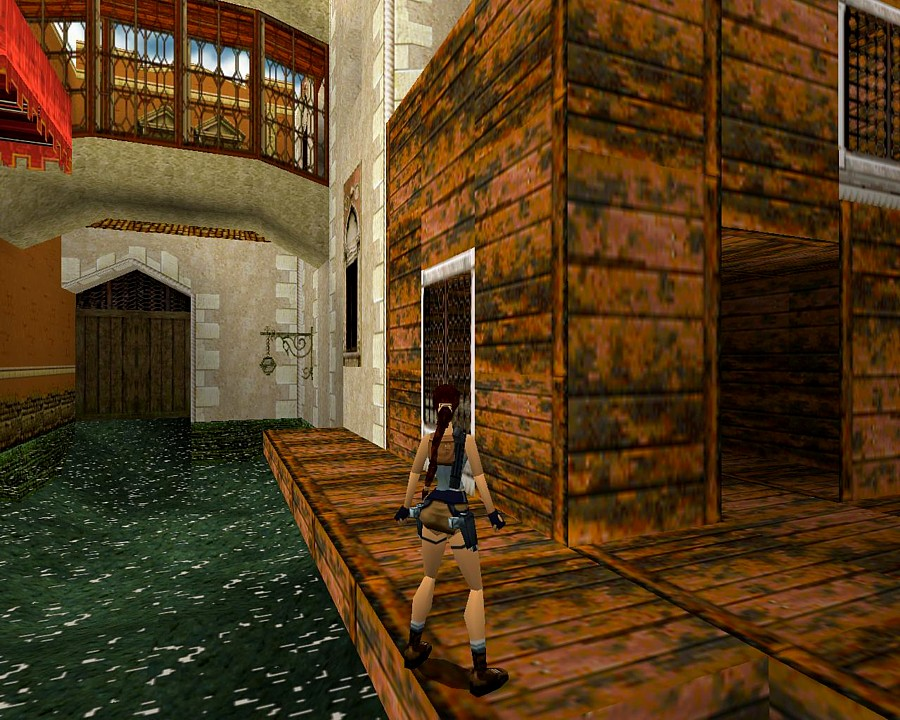
\includegraphics[width=.95\linewidth]{images/oldGraphics}
      \caption{Tomb Raider II (1997)}
      \label{fig:intro_tomb}
  \end{subfigure}
  \begin{subfigure}{.55\textwidth}
      \centering
      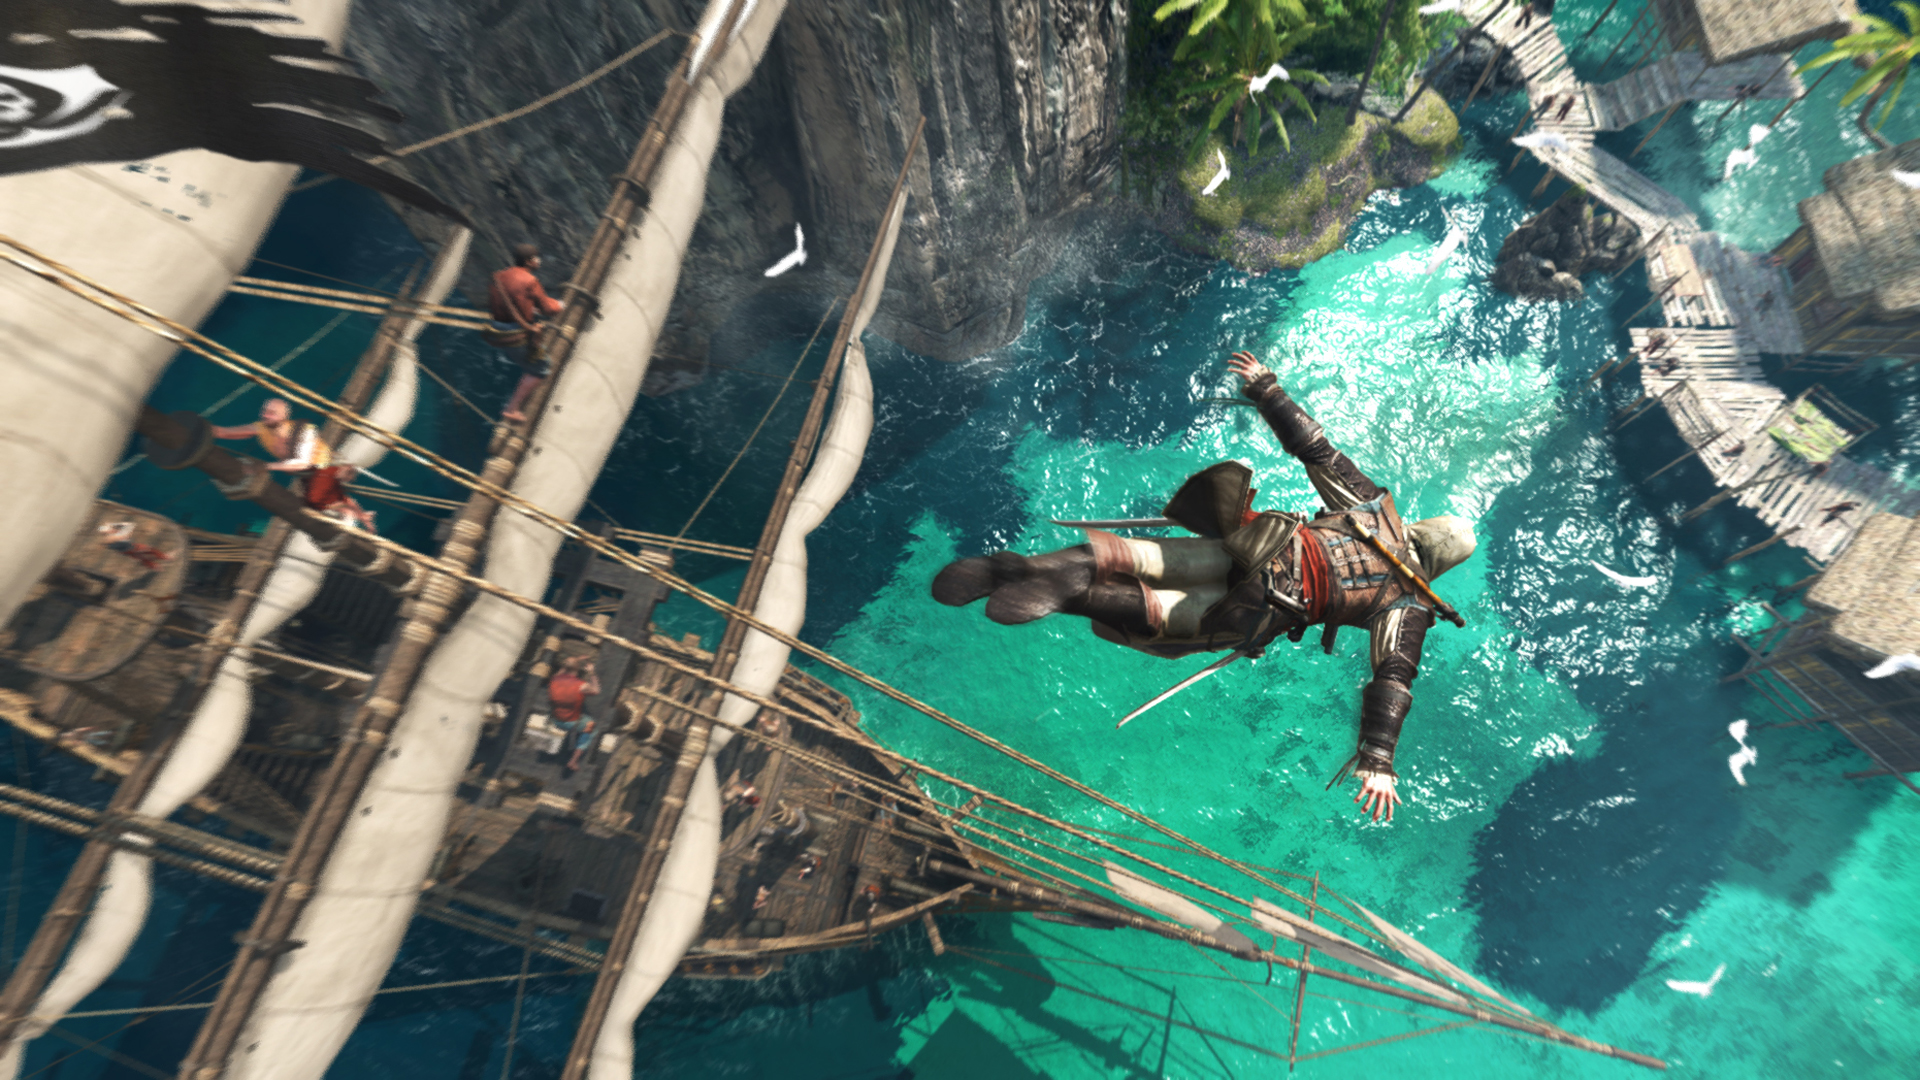
\includegraphics[width=.95\linewidth]{images/modernGraphics}
      \caption{Assassin's Creed (2014)}
      \label{fig:intro_assassin}
  \end{subfigure}
  \caption{Comparison of complexity of video game graphics. Modern GPUs can display graphics that are more complex, by several orders of magnitude.}
  \label{fig:intro_videogamecomp}
\end{figure}

Some years later, Pixel and Vertex shader units were unified into more general purpose unified Shader units, and around the same time the term of General Purpose GPU (GPGPU) Computing came into use. Microsoft introduced the DirectCompute API, NVidia the CUDA API and the Khronos Group the OpenCL API to enable developers to move parts of the execution of their programs to the GPU. All of these APIs enabled the programmer to execute general purpose code on the GPU without having to use facilities and APIs designed to display graphics. All of them use a C like language that is compiled for the individual GPUs at run time. \cite{khronos2008release,khronos2012specification,nvidia2009opencl} \\
\newpage



%%%%%%%%%%%%%%%%%%%%%%%%%%%%%%%%%%%%%%%%%%%%%%%%%%%%%%%%%%%%%%%
\section{Motivation}
\label{sect:intro_motivation}

Code executed in such a matter can be significantly faster than normal sequential code, especially if it is heavy on computations. Unfortunately, there is a rather high overhead, as resources need to be transferred to the device\footnote{The computing device used, for example the GPU of the PC.}. Figure \ref{fig:intro_performance_cpu_gpu} compares the execution time of applying an operation on every element of a two-dimensional array, with different sizes, using conventional methods and with the execution using a GPU and OpenCL. The first thing one notes is that the overhead alone makes it not viable to perform kernels on the GPU for small arrays. For these arrays, in this example those with less than about $5*10^4$ elements, the time spent on copying alone is larger than just executing the whole computation conventionally using the CPU. For larger arrays, there is a significant benefit to performing the computation on the GPU. This is especially true when comparing just the execution of the operation. If there is more then one operation that is performed on the GPU, and the data is already on the GPU, then the difference in execution time is about a single order of magnitude.\\

\begin{figure}[h]
  \begin{center}
    \begin{tikzpicture}
      \begin{loglogaxis}[ xlabel=Number of Elements, 
              ylabel=Time in µs,
              legend entries={CPU Total, GPU Total, GPU Execution},
              legend style={at={(1.03, 0.5)}, anchor=west}]
        \addplot [red, error bars/.cd, y dir=both, y explicit] table [x=elements, y=cpu, y error=cpuStdDev]{data/cpugpu.csv};
        \addplot [blue, error bars/.cd, y dir=both, y explicit] table [x=elements, y=gpu, y error=gpuStdDev]{data/cpugpu.csv};
        \addplot [green, error bars/.cd, y dir=both, y explicit] table [x=elements, y=run, y error=runStdDev]{data/cpugpu.csv};
      \end{loglogaxis}
    \end{tikzpicture}
    \caption{Execution time for the execution of a kernel with different number of elements. The red graph shows the time spent on executing the kernel on the CPU, using parallel for loops and vectorization. The blue graph shows the total execution time for the GPU, including the transfer of the memory to and from the device. The green graph shows the time spent executing the kernel on the GPU.}
    \label{fig:intro_performance_cpu_gpu}
  \end{center}
\end{figure}

There are, however, some downsides to executing code on the GPU. There is still a great amount of boilerplate code involved when writing OpenCL code. A lot of repetitive calls to C APIs need to be made, memory needs to be managed manually, work-group sizes determined and kernels enqueued for execution. Additionally, it may not always be a good idea to outsource the computation. OpenCL has certain restrictions, and is not suited for every kind of computation. Additionally, as seen above, there might not even always be a performance benefit. This thesis is part of an effort to address these concerns by implementing a compiler that automatically generates code both for the CPU and the GPU\footnote{See chapter \ref{chap:compiler}}, and selects the right kind of execution based upon the available resources and the program that is executed. Deciding whether to execute a computation on the GPU requires knowledge about the costs that come with the execution. Chapter \ref{chap:model} presents such a model. 
% !TEX root = ../main.tex

\chapter{Theory}
\label{chap:theory}

In this chapter the technologies, programming languages and algorithms that form the foundation for this thesis will be explained in detail. The underlying technology used to perform GPGPU computing is the  OpenCL\footnote{OpenCL homepage: \url{https://www.khronos.org/opencl/}} computing environment. As the intent of the thesis is to provide runtime predictions for a scheduler in a compiler, the other important part is that compiler and the programming language it belongs to, the FunkyIMP\footnote{FunkyIMP homepage: \url{http://www2.in.tum.de/funky}} programming language. 
%Foundation okay?


%%%%%%%%%%%%%%%%%%%%%%%%%%%%%%%%%%%%%%%%%%%%%%%%%%%%%%%%%%%
\section{OpenCL}
\label{sect:theory_opencl}
OpenCL was originally released by Apple in 2008 in conjunction with the 10.6 release of OS X. Subsequently, stewardship for the project was transferred to the Khronos Group, which is also responsible for OpenGL, and then released as an open standard for general purpose GPU computing. It is now widely used, with implementations for the major operating systems, as well as a wide range of devices. There are implementations by Apple for OS X, and by NVidia, AMD and Intel for their GPU and CPU products, respectively. \cite{khronos2008release,apple2013opencl} \\

Thus, in contrast to other GPGPU computing frameworks such as the CUDA framework maintained by NVidia, OpenCL is not constricted to a single vendor or type of device. A valid OpenCL kernel may be executed on any device that supports OpenCL, without the need for modifications. This makes the technology viable to be used in an environment with a multitude of heterogeneous devices, enabling an on-demand distribution of data parallel tasks onto available devices. \cite{vejarano2013parallel} \\

The following sections will give an overview of the OpenCL architecture, its execution model, memory model, and the C dialect used to write OpenCL kernels.

\subsection{The OpenCL platform architecture}
\label{sect:theory_opencl_platform}
The OpenCL platform consists of a host and multiple devices. Figure \ref{fig:theory_platform_model} illustrates the basic architecture. The Platform, also referred to as Host, is the environment the main program is executed on. It is not an OpenCL device itself, and the code does not have to be written in OpenCL. Any Programming language can be used, although the APIs for interfacing with OpenCL are written in C. There are wrappers for other Programming languages, such as C++. The platform uses these APIs to control the devices. \cite{khronos2012specification} \\

The Devices execute the actual data parallel programs, also known as kernels. Devices are hardware entities such as a GPU, a CPU or accelerators (in embedded environments) that can perform computations on their own. Each device consists of one or more execution units. For example, an execution unit may map to a core of a CPU. These execution units in turn have a number of ProcessingElements, each of which models the most fine-grained element of parallelism, e.g. a Shader Core. ProcessingElements may be called in a SIMD (\textbf{S}ingle \textbf{I}nstruction \textbf{M}ultiple \textbf{D}ata) fashion resulting in a completely parallel execution or in a SPMD (\textbf{S}ingle \textbf{P}rogram \textbf{M}ultiple \textbf{D}ata) fashion, wherein each ProcessingElement retains its own Program Counter. \cite{khronos2012specification} \\

For an example configuration of the platform architecture, see figure \ref{fig:platform_example} in the Appendix.

\begin{figure}
	\begin{center}
		\begin{tikzpicture}
			\begin{class}{Platform}{7,0} 
				\attribute{name : const char*}
				\attribute{vendor : const char*}
			\end{class}
			\begin{class}{Device}{0,0}
				\attribute{name : const char*}
				\attribute{vendor : const char*}
				\attribute{deviceType : DeviceType}
			\end{class}
			\begin{class}{ExecutionUnit}{0, -4.5}
				\attribute{processingElements: int}
			\end{class}
			\composition{Platform}{}{*}{Device}
			\composition{Device}{}{1..*}{ExecutionUnit}
		\end{tikzpicture}
	\end{center}
	\caption{UML class diagram of the OpenCL platform}
	\label{fig:theory_platform_model}
\end{figure}

\subsection{The OpenCL execution model}
In order to execute code in OpenCL, the following resources need to be managed:
\begin{itemize}
	\item The \textbf{device} that is to be used for the computations.
	\item The \textbf{kernel}, a function that is to be executed on the OpenCL device.
	\item The \textbf{program}, the actual source of the program that is to be executed.
	\item The \textbf{memory} objects the kernel is executed on.
\end{itemize}
This functionality is bundled in the so-called \textbf{context}. Interactions with the device are done using \textbf{command queues}. These are used to execute operations, manage the device's memory, or to determine the order the commands are executed in. \cite{khronos2012specification} \\

The OpenCL programs are written in OpenCL C, which will be discussed in detail in section \ref{sect:theory_opencl_c}. They are then executed in parallel over a defined computation domain with each thread, also known as \textbf{work item}, handling one element of that domain. This element might be a single computation on one value in an array, or more involved operations on a column in a matrix. The work items are again grouped into \textbf{work-groups}\footnote{Sometimes also known as wave fronts.}, which enable synchronization within a work-group. There is also a level in the memory hierarchy that is shared within a work-group. The different work-groups on the other hand are completely independent from each other. As there are many threads executed at the same time, they usually share one program counter, executing the same instruction on multiple threads at once. This has some interesting effects. If there are control structures or branches in the code, every branch will still have to be executed, and results of the computations will have to be canceled out if the computation is not to be done on that particular work item. This also translates to performance penalties for very control-flow-heavy programs. \cite{tompson2012introduction}

\subsection{The OpenCL memory model}
\label{sect:theory_opencl_memory}

\begin{figure}
	\begin{center}
		\includegraphics[width=0.75\linewidth]{images/memory_hierarchy}
	\end{center}
	\caption{The OpenCL memory hierarchy.}
	\label{fig:theory_memory_hierarchy}
\end{figure}

An important design aspect for OpenCL is the closeness to the hardware. This implies the need for a memory architecture that maps well to real graphics hardware. To achieve this, a multi-layer memory architecture has been chosen. Consider figure \ref{fig:theory_memory_hierarchy} for an overview. The fastest type of memory is the \textbf{private memory}. Every work item has its own, and it is typically the part of memory where all local variables and parameters used in a kernel are stored. For a NVidia graphics card, the access time would typically be comparable to a register access. However, this is not guaranteed. \cite{tompson2012introduction,nvidia2009opencl} \\

Next in the memory hierarchy is the local memory. This part of memory is shared amongst the work items of a single work-group. On NVidia graphics cards, local memory is located in the off-chip DRAM, resulting in longer latencies for memory accesses, typically around 200-300 cycles. \cite{nvidia2009opencl,hwu2009compute} \\

There also is a special area of memory reserved for constant data. Data in Constant memory is immutable for the duration of the kernel execution, and can thus be cached for quicker access. This usually results in shorter latencies, for NVidia graphics cards it is usually about as fast as a register access. \cite{hwu2009compute} \\

Lastly, there is the Global Memory. It has the greatest amount of available memory, and it is shared across the whole device. On NVidia graphics cards it is usually implemented as a dedicated off-chip DRAM. This implies a high access latency, and as with the local memory, it is around 200-300 cycles.
\cite{hwu2009compute,tompson2012introduction} \\

It is also notable that there is no concept of memory protection on the GPU. Segmentation faults are not reported, that means if a work item modifies a memory segment outside of its own memory segment, anything can happen, up to and including gibberish on the screen or a full crash of the operating system. When implementing a new OpenCL kernel, it is usually a good idea to test it on a CPU device first, as those usually implement memory protection, and a segmentation fault will be reported instead of causing random undefined behavior on the system. \cite{tompson2012introduction}

\subsection{The OpenCL C dialect}
\label{sect:theory_opencl_c}
OpenCL kernels are written in a slightly modified version of C99, a language called OpenCL C. It features some additional data types for handling vector types, as well as well as implementations for basic operations on them. Vectors can have a length of 2, 3, 4, 8 or 16. The following data types are supported: \code{char}, \code{short}, \code{int}, \code{long} and their unsigned counterparts, as well as \code{float} for floating point values. The operations are the usual operators, and they are applied component-wise (see equation \ref{eq:theory_vector_add}). \cite{khronos2012specification} 
\begin{gather}
	\label{eq:theory_vector_add}
	\begin{pmatrix}
		a_1\\
		a_2\\
		a_3\\
		a_4
	\end{pmatrix} + 
	\begin{pmatrix}
		b_1\\
		b_2\\
		b_3\\
		b_4
	\end{pmatrix} =
	\begin{pmatrix}
	a_1+b_1\\
	a_2+b_2\\
	a_3+b_3\\
	a_4+b_4
	\end{pmatrix}
\end{gather}
There are several limitations as well, the most important one shall be explained here. For the full list, see \cite{khronos2012specification}. In OpenCL, function calls are implemented via inlining, that means that functions that are called from within a kernel simply have their body copied into the original kernel, replacing the parameters by the function call arguments. This implies two limitations. The inlining has to be a finite process, that means that \emph{recursion is not possible}, specifically, there may not be any cycles in the function call graph. It also means that all the called code has to be known at (kernel) compile time. The second implication is therefore the impossibility of function pointers, as they would enable the programmer to call any code at runtime, thus rendering the inlining impossible. There are some more limitations for pointers. They may only be declared in conjunction with either the \code{global}, the \code{local} or the \code{private} address space qualifier. Pointers of one address space specifier may not be assigned to a pointer with a different address space specifier.  \cite{khronos2012specification} \\ %Font? Fett?

Figure \ref{fig:theory_opencl_kernel} shows a very simple OpenCL kernel. It illustrates several elements that are common to all kernels. In the function signature, kernels are marked as such using the \code{kernel} keyword. The return type of a kernel is always \code{void}. Parameters are used for the communication between the kernel and the host. There are parameters that point to the data transferred to the GPU by the host, and a pointer to the memory segment that is to hold the result. By default, the parameters reside in the \code{private} address space. The \code{constant} and \code{global} address space specifiers denote the type of memory the pointers are pointing to. Local variables, such as \code{work\_item\_id} are also in the \code{private} address space by default. The function \code{get\_global\_id(0)} is called to determine the id of the current work item. \cite{khronos2012specification} %Font?


\begin{figure}[hb]
	\lstset{language=c}
	\lstset{morekeywords={kernel}}
	\lstset{morekeywords={global}}
	\lstset{morekeywords={constant}}
	\begin{lstlisting}
kernel void vector_add(constant float *a, constant float *b, 
				global float *c)
{
	int work_item_id = get_global_id(0);
	c[work_item_id] = a[work_item_id] + b[work_item_id];
}
	\end{lstlisting}
	\caption{This is an example of an OpenCL-Kernel. It adds the content of two vectors and writes the result into a third one. \code{get\_global\_id(0)} returns the current work item number, in this case it corresponds to the position in the arrays.}
	\label{fig:theory_opencl_kernel}
\end{figure}
\newpage



%%%%%%%%%%%%%%%%%%%%%%%%%%%%%%%%%%%%%%%%%%%%%%%%%%%%%%%%%%%
\section{The FunkyIMP programming language}
\label{sect:theory_funky}
The FunkyIMP programming language is developed by Alexander Herz as a race and deadlock-free, implicitly parallel, functional programming language. It employs task as well as data parallelism in order to maximize the number of computations that are executed in parallel. This is done without losing the ability to handle I/O and events. Thus funkyIMP can be considered a general purpose programming language. For this thesis, the type system, with its polyedric array domains, is of most interest. It is explained below. \cite{herz2013funkywiki} \\ %Should also be okay, they are not the whole type system.

Most functional languages use single linked lists as their main way of storing data in bulk. For these lists, a wide range of operations, such as \code{map}, \code{filter} or \code{foldl}\footnote{For descriptions of those functions, please see \ref{sect:appendix_functional}} are available. These operations enable the programmer to write very concise, declarative code, focusing on what to achieve instead of how to do it. A simple example of this is the reversing of lists. Using functional code with lists, this can be expressed as below. The example is written in Standard ML.

\lstinputlisting[language=ml, tabsize=2]{code/reverseList.sml}

The code is short and very declarative, and the meaning should be clear at first glance. However, the implementation of the same functionality is more difficult with arrays. In Standard ML, arrays are declared in the structure \code{Array}. To reverse an array, one has to write code such as the following.

\lstinputlisting[language=ml, tabsize=2]{code/reverseArray.sml}

This code is much more complicated. It needs to use array indices and several temporary variables. Additionally, \code{Array}s are mutable in SML, and the implementation has to make use of this. To sum it up, the declarative nature of the code is largely absent, instead it is solved with an iterative approach. With that added complexity comes several possible problems. First, consider \code{(*1*)}. This line will fail to execute if the array has zero elements, a case that should be handled using a conditional statement as well, otherwise the execution will fail with an exception at run time. The other index operations also need to perform bounds checks at runtime, and would raise exceptions if the accesses were outside the array bounds. Programming errors like that can easily happen, for example one might forget to subtract the 1 at line marked with \code{(*2*)}.\\

How does this complexity arise? In most programming languages, arrays are treated as one-dimensional pieces of memory, just as in the example above. In a functional environment, and with immutable values, the actual structure with which the values are saved in memory might not matter too much. It may be more important to have a type system that enables reasoning about array size and structure at compile time, enabling the programmer to create subarrays that fulfill certain criteria, and to perform operations on them. In other cases, such as the reverse example, it might be enough to provide a different way to address the original array. \\

FunkyImp allows the programmer to do that. Given an one-dimensional array defined as 
\begin{gather*}
	\operatorname{domain} \ arr_{1D}\{x\}() = \{(i) : i < x\}
\end{gather*}
one can define the reversed array as follows:
\begin{gather*}
	\operatorname{domain} \ arr_{rev}\{x\}() : arr_{1D}(a) = \{arr_{1D}\{x\}(i) : a = x-i-1\}
\end{gather*}
Now all the programmer needs to do is create a new variable and cast the old value into the new one, e.g.:
\begin{verbatim}
int[arr_1D{10}] x = new int[arr_1D{10}];
int[arr_rev{10} y = (int[arr_rev{10}]) x;
\end{verbatim}

\subsection{Multidimensional Arrays}
\label{sect:theory_funky_multidim}

Multidimensional arrays are another problem that are efficiently solved by polyedric domains. This is shown with the implementation of a matrix as an example. There are several different approaches to solve this problem. These will be illustrated with the following example:
\begin{align*}
	M &\in \real^{3\times4} \\
	M &= \begin{pmatrix}
			1 & 2 & 26 & 4 \\
			5 & 6 & 14 & 8 \\
			42 & 7 & 3 & 89
		\end{pmatrix}\\
	v &= M_{i,j}
\end{align*}

The least involved approach is to simply implement the matrix as a one-dimensional array. In an imperative language such as C, it might be implemented as follows:

\lstinputlisting[language=c, tabsize=2]{code/simpleMatrix.c}

This approach is the most simple one to implement in the compiler, but leaves most of the computational burden for the programmer. For one, the structure of the matrix is not expressed in the type of \code{M}. If the programmer wants to use the matrix in another function, they will have to manually transfer all the information about the structure of the matrix to that other function. If that is not done, nothing prevents the programmer from interpreting the matrix as, say, for example, a $\real^{6\times2}$ matrix. Additionally, array access is not straightforward. Again, the programmer has to maintain the semantic meaning of the array. If they want to access an element of the matrix, they will have to compute the right index for the array index themselves. To sum it up, this is the approach that is closest to the actual memory structure of the computer, but it does assume careful attention by the programmer. \\

Another approach is to implement the matrix as an array of arrays. This might be implemented as follows, for example in Standard ML:

\lstinputlisting[language=ml, tabsize=2]{code/arrayOfArraysMatrix.sml}

This approach is still quite simple to implement from a compiler point of view. It has several advantages from a type safety point of view. It is now no longer possible to reinterpret the matrix as something other than a two-dimensional array with the given dimensions. This type safety, however, comes at a cost. It is now no longer guaranteed that the matrix is stored in one continual segment of memory. That might have negative side effects on the performance. Additionally, from a semantic standpoint, an array of arrays is still a slightly different concept than a two-dimensional array. \\

The FunkyIMP approach combines type safety while still retaining the continuous memory segment by taking the address computations out of the programmer's hands and generating the necessary code during complilation. It might be implemented as follows:

\lstinputlisting[language=java, morekeywords={domain}]{code/funkyArray.funky}

The first line defines a simple one-dimensional array. Usually, that will be predefined. The second line describes a two-dimensional array with $a$ rows and $b$ columns. It inherits the properties of a one-dimensional array with the length of $a*b$. Then, constraints for the indexing parameters are specified. Here, the parameters may only be within the limits set by $a$ and $b$. Constraints specifying that $x,y \geq 0$ are implicitly added. In line 3, the newly created domain is used to build a matrix with a size of $4\times3$. After the values are initiated, the programmer can simply retrieve them using an indexed access. %Should be okay in this context.
 This solution captures the semantics of a matrix, while still retaining the runtime benefits of the C implementation, as it basically performs the same index computations. In contrast to the C example, here they are generated by the compiler.

\subsection{Map and Reduce}
\label{sect:theory_funky_mapreduce}
Recall the listing from the beginning of section \ref{sect:theory_funky}. It describes several operations typically implemented on lists in functional programming languages, namely \code{map}, \code{filter} and \code{foldl}. They provide a simple and easily understandable way to iterate on lists. These operations (except for \code{filter}\footnote{It does not make too much sense to remove elements from an array that cannot be resized.}) on arrays are implemented as language features in funkyIMP.\\

To illustrate their functionality, the following operations will be performed, the first using map and the second one using reduce.
\begin{gather*}
	M = \begin{pmatrix}
			1 & 2 & 3 \\
			4 & 5 & 6 \\
			7 & 8 & 9
		\end{pmatrix}^T\\
	v = \sum_{m_{ij} : i, j \in \nat_3 } m_{ij}
\end{gather*}  

The code looks as follows:

\lstinputlisting[morekeywords={reduce, int, new,}]{code/mapreduce.funky}

The \verb!.\! performs the map operation. It returns a new Array with the same type as the old one. The second operation, the \verb!.\reduce! describes how to collect the contents of the array into a single value. \\

For this thesis, the \code{map}-Operation\footnote{Also referred to as a domain iteration in later chapters.} is considered the most interesting. The original matrix is immutable and the new value only depends on the old matrix (and other, also immutable, variables). Hence the operation may be parallelized readily. Chapter \ref{chap:compiler} will highlight the steps to be taken in order to incorporate the generation of code for the GPU-accelerated \code{map}-operation into the funkyIMP compiler. 

%% ---------------------------------------------------------------------------
%%
%% Description of the implementation
%%
%%% ---------------------------------------------------------------------------
\part[Methodology]{Methodology}
\label{part:methods}
% !TEX root = ../main.tex

\chapter{Extensions to the funkyIMP Compiler}
\label{chap:compiler}
The funkyIMP compiler is a heavily modified version of the Java compiler. Its front end has been customized to parse code that adheres to the funkyIMP language specification. More pertinent for this thesis is the compiler back end. It has been replaced completely to emit C++11-compatible code instead of Java byte code. This generated code is then compiled to native machine code using a GNU g++ compiler. In order to support the execution of code on the GPU, several modifications had to be made to the existing code base. This chapter will discuss them in detail, starting with the overview of the process at a high level, and then explaining each component individually.



%%%%%%%%%%%%%%%%%%%%%%%%%%%%%%%%%%%%%%%%%%%%%%%%%%%%%%%%%%%
\section{System Overview}
\label{sect:compiler_overview}
Offloading a computation to the graphics card takes several steps. In the beginning, one must gather all the necessary data and code that will be used in the computation. To do this, all symbols used in the computation need to be collected, including those found in functions called within the original kernel. Functions need to be translated into OpenCL-C, local variables are passed as parameter and memory segments need to be processed and copied to the GPU. As OpenCL does not have a sophisticated array type system, some additional information such as the size of the array in bytes need to be computed. Afterwards, code to allocate space on the GPU to copy the content of the array on host side to the GPU is generated. Further steps to generate the code on the host side include the allocation of space for the computation results on the GPU, the actual invocation of the computation, and the copying of the result of the computation back to the host. \\

In addition to the generation of the boilerplate code to invoke the OpenCL kernel, code for the actual kernel itself needs to be generated as well. This is done, in accordance with the rest of the compiler architecture, by utilizing the Visitor Pattern\footnote{As defined in \cite{gamma1994design}}. It iterates over the Syntax tree, generating code recursively. \\

There also is a runtime component for the funkyIMP language. There is a library\footnote{See C++ Wrapper \cite{medina2013wrapper}} that encapsulates the OpenCL API calls with a simple object-oriented C++ API. The library has been slightly changed to incorporate some additional features, such as querying frequently needed device information. \\

The following sections will give a detailed overview of the additions to the funkyIMP compiler developed in the course of this thesis. They will follow the steps the compiler performs to output the necessary C++ code. 
\newpage



%%%%%%%%%%%%%%%%%%%%%%%%%%%%%%%%%%%%%%%%%%%%%%%%%%%%%%%%%%%
\section{Code generation for the Host}
\label{sect:compiler_code}
This section details the generation of code to handle the host side of the kernel execution, the compilation of the kernel, its execution, and the management of the necessary variables. 

\subsection{Collection of Identifiers}
\label{sect:compiler_code_identifiers}
The first step to be performed is to collect all the identifiers needed for the execution of the kernel. There are several types of identifiers to be considered. The first type is the \textbf{local variable}. Local variables are self-contained values that can be set simply as a parameter for the kernel. The second type of identifier is the \textbf{array}. Arrays are also set as a parameter. In addition, the memory segments they point to need to be copied to the GPU. The third type of identifier holds \textbf{functions}. In the function body, other functions, arrays or local variables may be accessed too. This necessitates an analysis of the body of the function for identifiers. Functions also need to be compiled. The last type of identifiers to be considered are \textbf{Iteration Arguments}. These need not be copied, as they can be computed from the work item id of the kernel. They will be computed on the GPU at runtime.\\

To gather the necessary information about the kernel, the following analysis is performed. Let $\mathcal{V}$ be the set of all the possible syntactical elements of the language (e.g. Identifiers, keywords, Literals, ...) and let $\mathcal{T}$ be the set of all syntax trees defined as in equation \ref{eq:syntaxtree}. Let $\mathcal{L} \subseteq \mathcal{V}, \mathcal{A}\subseteq \mathcal{V}, \mathcal{F}\subseteq \mathcal{V}$ be the set of all local variables, the set of all arrays and the set off all functions, respectively. Let $\mathcal{I}$ denote the set of iteration parameters of the domain. An abstraction of the syntax tree looks as follows:
\begin{align}
v &\in \mathcal{V}\notag\\
t &=\begin{cases}
		\Node(v, t_1, \dotsc, t_n) \\
		\Leaf(v)
	\end{cases}
	\label{eq:syntaxtree}
\end{align}
With those definitions the set of all identifiers needed in a kernel, denoted as  $\mathcal{E} \subseteq \mathcal{L} \cup \mathcal{A} \cup \mathcal{F}$, can be computed as can be seen in equation \ref{eq:compiler_identifier_analysis}. Intuitively, the syntax tree is iterated over, and in the case where there are any identifiers that denote functions, their bodies will also need to be checked for identifiers as. For an example, see \ref{ex:identifiers} in the appendix.\\
\begin{figure}[H]
	\begin{align}
		\llbracket \Node(T_1, T_2, \dotsc T_n) \rrbracket^\sharp &= 
			\llbracket T_1\rrbracket^\sharp \cup \llbracket T_2 \rrbracket^\sharp \cup \dotsb \cup \llbracket T_n\rrbracket^\sharp &\quad \label{eq:compiler_identifier_analysis} \\
		\llbracket \Leaf(i) \rrbracket^\sharp &= 
			\{i\} &\quad (i \in \mathcal{L} \cup \mathcal{A}) \notag\\
		\llbracket \Leaf(f) \rrbracket^\sharp &= 
			\{f\} \cup \llbracket\operatorname{resolve}(f)\rrbracket^\sharp &\quad (f \in \mathcal{F}) \notag\\
		\quad&\quad&\quad \notag\\
		resolve &: \mathcal{F} \rightarrow \mathcal{T} &\quad \notag\\
		resolve (f) &= t_f &\quad \text{where $t_f$ is the body of $f$.} \notag
	\end{align}
	\caption{Analysis to extract the set of used identifiers from an expression.}
\end{figure}

Some of the identifiers captured in $\mathcal{E}$ may not be necessary. The iteration arguments are generated on the GPU at runtime, as they depend on the number of the work item they are executed upon. Hence, they need to be taken from the set. Additionally, any variables that are locally defined in called functions may be taken from the set as well. This yields the final set of needed identifiers $\mathcal{E}^* = \mathcal{E} \setminus (\mathcal{I} \cup \mathcal{L}_{local}$


\subsection{Code for needed variables}
\label{sect:compiler_variable_init}
All array variables that need to be copied to the GPU have to be processed. They have to be mapped to the more simple, C-style memory segment while keeping the information about the array's structure intact. Specifically, the lengths of the array's dimensions need to be obtained. Additionally, code for the allocation of the memory on the GPU has to be generated. For the purpose of code generation, with $\mathbb{T}_p$ denoting the set of primitive types (e.g \code{float}, \code{int}, \code{double}, \code{char},...), an array may be described as follows.
\begin{gather*}
	A = \langle m, d, T \rangle \\
	T \in \mathbb{T}_p, d \in \nat^n, m \in T^{s}\ where\ s = \prod_{k=1}^n d_k
\end{gather*}
With this definition the code generation function $code_{Host}$ for array variables can be defined as given in equation \ref{eq:compiler_code_array}. The first step is to extract a simple pointer to the array's memory segment using the FunkyIMP runtime method \code{toNative()}. The next step is to allocate enough space on the GPU to fit the memory segment just extracted. The total size of that segment is calculated from the size of the primitive data type of the array and the product of the sizes of each dimension. Additionally, for each dimension, a local variable, holding its size, is allocated. Finally, the memory segment is copied over to the GPU. \\

Code generation for local variables with a primitive type is less complex than conde generation for arrays. They can be defined as $L = \langle T, v\rangle$ with $T \in \mathbb{T}_p$ and $v\in T$. Their code generation function is given in equation \ref{eq:compiler_code_local}.\\


\begin{align}
\label{eq:compiler_code_array}
code_{Host}\ A\ = &\ T\ *m = A\rightarrow \operatorname{toNative();} \\
           				&\ \text{ocl\_mem}\ m_{GPU}\ = \notag\\
           				&\ \qquad\operatorname{device.malloc}\left (\operatorname{sizeof}\left(T * \prod_{k=1}^n d_k\right),\operatorname{CL\_MEM\_READ\_ONLY}\right);\notag\\
            			&\ \operatorname{int} m_{dim_0}= d_1;\notag\\
            			&\ \qquad\vdots\notag\\
            			&\ \operatorname{int} m_{dim_n}= d_n; \notag\\
            			&\ m_{GPU}\operatorname{.copyFrom}(m);\notag\\
            			&\ \notag\\
	\label{eq:compiler_code_local}
code_{Host}\ L\ = &\ T\ a = v;
\end{align}



\subsection{The return value}
The return value of a kernel has to be treated slightly differently. There is no direct counterpart on the host, as the object is created by the domain iteration. Hence, memory for the return value needs to be allocated on the GPU as well as on the host. In contrast to the arrays in the section above, the memory is not allocated in read only mode but in write only mode. The return value cannot be referenced from funkyIMP code, so it is not necessary to make it readable. In addition, the memory is not initialized to anything and contains undefined values. \\

\begin{align}
\label{eq:compiler_code_return}
code_{Host}^{begin}\ R\ = &\ T\ *ret = \operatorname{new}\ T\left[\prod_{k=1}^n d_k\right];  \\
           			&\ \text{ocl\_mem}\ ret_{GPU}\ = \notag\\
           			&\ \qquad\operatorname{device.malloc}\left (\operatorname{sizeof}\left(T * \prod_{k=1}^n d_k\right),\operatorname{CL\_MEM\_WRITE\_ONLY}\right);\notag
\end{align}


The return value needs to be copied back to the host after the computation, and then also translated back into a format compatible with the funkyIMP runtime. The code generation function is shown in equation \ref{eq:compiler_code_return_2}. First a new \code{LinearArray} object is created. Then a new \code{Version} object ($ret_{funky'}$) is built. It is a version of the array enriched with information about the structure of the array, and the value that is returned as the result of the computation.

\begin{align}
\label{eq:compiler_code_return_2}
code_{Host}^{end}\ R \ = 	&\ ret_{GPU}\operatorname{.copyTo}(ret);\\
				 	&\ \operatorname{funky}::\operatorname{LinearArray}<T> *ret_{funky} = \notag\\
				 	&\ \qquad \operatorname{new} \operatorname{funky}::\operatorname{LinearArray}<T>\left(\prod_{k=1}^n d_k,ret\right); \notag\\
            		&\ \operatorname{funky}::\operatorname{LinearArray}<T>::\operatorname{Version}\ * ret_{funky'} = \notag\\
            		&\ \qquad \operatorname{new} \operatorname{funky}::\operatorname{LinearArray}<T>::\operatorname{Version}(ret_{funky},n,d_1,\dotsc, d_n); \notag
\end{align}

\subsection{Code generation for the Domain iteration}
\label{sect:compiler_code_program}
There are more tasks that need to be performed apart from the allocation of variables. The actual code for the GPU needs to be compiled and the parameters set, and then the code needs to be executed. Equation \ref{eq:compiler_code_whole} shows the code generation function $code_{Host}$, a formal definition of the whole process. The kernel is first compiled for execution on the target device. Then code for all variables gathered with the analysis presented in section \ref{sect:compiler_code_identifiers} will be generated. The process is similar for the allocation of the return value. Afterwards, the kernel arguments need to be set. For primitive variables it is enough to pass the address they are stored at, while for an array the actual OpenCL memory object and the variables holding its dimensions need to be given. Subsequently the kernel is executed with $|R|$ work items and a work group size that is the greatest even divider of the number of work items that is less than or equal to the maximum work group size of the GPU $W_{max}$. Section \ref{ex:generated_code} in the appendix shows the actual output of the code generation process for a domain iteration. The identifier names in the output generated by the compiler differ slightly from the ones in the hypothetical output of the the code generation function $code_{Host}$ specified in this section. This deviating naming schema is utilized in the implementation to avoid duplicate identifier names. \\ %Certain about that ???

\begin{figure}
	\begin{align}
		\label{eq:compiler_code_whole}
		code_{Host}\ P\ = 	&\ \operatorname{ocl\_kernel}\ k( \& device, \text{``tmp/k.cl''});\\
							&\ code_{Host}\ V_1 \notag \\
							&\ \qquad \vdots \notag \\
							&\ code_{Host}\ V_n \notag \\
							&\ code_{Host}^{begin}\ R \notag \\
							&\ k\operatorname{.setArgs}(args(V_1),\dotsc, args(V_n))\notag\\
							&\ k\operatorname{.run}(workgroup(|R|), |R|)\notag\\
							&\ \operatorname{device}.\operatorname{finish}();\notag\\
							&\ code_{Host}^{end}\ R \notag \\
							&\ \operatorname{return} ret_{funky'} \notag \\
							&\ \notag \\
		\label{eq:compiler_code_whole_idents}
		\left\{V_1, \dotsc, V_n \right\} = &(\abstsyntax{P}_{ident} \cup R) \setminus (\mathcal{I}\cup \mathcal{F})\\
		\label{eq:compiler_code_whole_args}
		args\ V = & 	\begin{cases} 
						\&V & V \in \mathcal{L} \\
						\quad\\
						\begin{matrix}	
							V.\operatorname{mem}()\\
							\&v_{dim_0} \\
							\vdots\\
							\&v_{dim_n} 
						\end{matrix} & V \in \mathcal{A}
					\end{cases} \\
		\label{eq:compiler_code_whole_workgroup}
		\left|\langle \_, d, \_\rangle\right| =	&\ \prod_{k=1}^n d_k \\
		workgroup\ n\ = &\ \operatorname{max}\left\{w |\ w > 0 \wedge w < n \wedge w < W_{max} \wedge w\mod n = 0 \right\} 
	\end{align}
	\caption{Code generation function for the whole domain iteration.}
\end{figure}
\newpage



%%%%%%%%%%%%%%%%%%%%%%%%%%%%%%%%%%%%%%%%%%%%%%%%%%%%%%%%%%%
\section{Code Generation on the GPU}
\label{sect:compiler_gpu}
In this section the part of the code generation that produces code for the GPU is explained. There are two steps to the process: The first step is to gather all the functions that are called from the kernel, and to build a dependency graph. The second step is to generate code for them and the kernel. The kernel is a function as well, but there are several special properties that need to be considered. 

\subsection{Dependent Function Analysis}
\label{sect:compiler_gpu_dependent_functions}
One of the most important ways to structure code is the use of functions and procedures. Unfortunately, support for function calling in OpenCL C is somewhat limited. Function calls will be inlined, and hence it is impossible to generate code for programs with recursive function calls. \cite{khronos2012specification} \\

This necessitates an analysis of the called functions. The call graph of a function can be obtained from the funkyIMP compiler. The call graph in general has the properties of a directed graph, each function being represented by a vertex, and each function call being an edge. All functions that are reachable from the kernel vertex\footnote{i.e $\Path(kernel, f)$} of the call graph need to be included in the translation. Recursion is not allowed, hence a way to detect it is needed. In terms of graph theory, a function $f$ is recursive iff $\Path(f,f)$. It can be seen that this is the case if the graph has a cycle. In case the graph is not recursive, the graph needs to be topologically sorted so that the code for functions can be generated in a way that makes forward declarations unnecessary.
\begin{small}
	\begin{align*}
		G &= \left\langle V, E \right\rangle,\ E \subseteq V\times V &\ \text{(A directed graph)} \\
		\Path(v_1,v_2) &\Leftrightarrow (v_1, v_2) \in E \vee \exists v':(v_1, v') \in E \wedge \Path(v', v_2) &\ \text{(Path between $v_1$, $v_2$)}\\
		\operatorname{DAG}(G) &\Leftrightarrow \neg\exists(v_1,v_2)\in E : \Path(v_1,v_2) \wedge \Path(v_1, v_2) &\ \text{(Directed Acyclic Graph)} \\
		\operatorname{Sorted}([v_1,\dotsc,v_n]) &\Leftrightarrow \neg\exists\ 1\leq k\leq n:\exists\ 1\leq l \leq n: \Path(v_l, v_k) &\ \text{(	Topologically sorted List)}
	\end{align*}
\end{small} 
Section \ref{ex:callgraph} in the appendix illustrates these principles with an example. The code generation for functions is discussed in the next section.

\subsection{Code generation for Functions}
\label{sect:compiler_gpu_functions}

For the compilation of functions there are two tasks that need to be performed. The first is to generate the function signature, the second to generate the function body itself. The first step will be described here, while the second step is covered below, in section \ref{sect:compiler_gpu_code_kernel}, where code generation for GPU kernels is described.

\paragraph{Function Headers} in C need to have a unique name, whilst funkyIMP allows overloaded functions. For this reason, the compiler needs to generate a unique name from the function specified in funkyIMP. Additionally, if there are any array types, they need to be translated to the appropriate pointer types. The code generation function is given in equation \ref{eq:compiler_code_function_header}.

\begin{align}
	\label{eq:compiler_code_function_header}
	code_{GPU}\ T_{ret}\ f(\operatorname{params})
		\{ \operatorname{body} \}\ = 	&\ code_{GPU}\ T_{ret} &\ \\
									 	&\ name \ (T_{ret}\ f(\operatorname{params})) &\ \notag \\
										&\ (code_{GPU} \operatorname{params}) &\ \notag\\
										&\ code_{GPU} \operatorname{body} &\ \notag\\
	code_{GPU}\ T\ = 					&\ T &\ (T\in\mathcal{T}_p) \notag \\
	code_{GPU}\ T\ =					&\ T * &\ (\text{for others}) \notag \\
	code_{GPU}\ \operatorname{params}\ =&\ code_{GPU}\ T_1\ t_1, &\ \notag\\
										&\ \qquad\vdots &\ \notag\\
										&\ code_{GPU}\ T_n\ t_n &\ \notag\\
	code_{GPU}\ \operatorname{body}\ =  &\ \{code_{GPU} (S_1;\dotsc S_m)\} \notag
\end{align}
\begin{align*}
	name (T_{ret}\ f(\operatorname{T_1 t_1, \dotsc T_n t_n})) &=\ T_{ret}\_f\_T_1\_\dotsc\_T_n
\end{align*}


\subsection{Code Generation for GPU Kernels}
\label{sect:compiler_gpu_code_kernel}
The kernel itself is also an OpenCL function, but it has some special properties. Some of these stem from OpenCL and some are limitations imposed by the manner in which funkyIMP handles the domain iterations. OpenCL states that kernels are to be marked with a special \code{kernel} keyword. It is also required that the return type of all kernels is void. The result is stored in a section of the global memory, and a pointer to that section is passed as a parameter. There are also some special considerations for the parameters. Arrays need the \code{global} address space specifier, whilst primitive values need no address space qualifier which makes them implicitly \code{private}. This leads to the slightly modified code generation function specified in equation \ref{eq:compiler_code_kernel_header}.

\begin{align}
	\label{eq:compiler_code_kernel_header}
	code_{GPU}\ T_{ret}\ f(\operatorname{params})
		\{ \operatorname{body} \}\ = 	&\ \operatorname{\_\_kernel} \operatorname{void} k &\ \\
										&\ (code_{GPU} \operatorname{params}, code_{GPU} V_{R}) &\ \notag\\
										&\ code_{GPU}^{kernel} \operatorname{body} V_R &\ \notag\\
	code_{GPU}\ V\ = 					&\ T_{V}\ n_V &\ (T_V \in\mathcal{T}_p) \notag \\
	code_{GPU}\ V\ =					&\ \operatorname{global} T_V * n_v, &\ (T_V \not\in \mathcal{T}_P)&\ \notag \\
										&\	\operatorname{int}\ V_{dim_0},&\ \notag \\
										&\	\qquad\vdots&\ \notag \\
										&\	\operatorname{int}\ V_{dim_n}&\ \notag \\					
	code_{GPU}\ \operatorname{V_1,\dotsc, V_n}\ =&\ code_{GPU}\ V_1, &\ \notag\\
										&\ \qquad\vdots &\ \notag\\
										&\ code_{GPU}\ V_n &\ \notag
\end{align}

The parameters $V_1$ to $V_n$ are equal to the ones specified in equation \ref{eq:compiler_code_whole_idents}. Their order is also identical. The name of the kernel ($k$) also matches the name of the kernel on the host side.\\ 

The code generation function given above does not define the code generation for the body of the kernel. In section \ref{sect:compiler_gpu_functions}, when translating helper functions, it was enough to simply compile the statements of the function. The domain iteration however is only an expression, not a series of statements, hence its result needs to be assigned to something so that it does not get lost. In this case it is the element of the return value that is currently processed. That element is determined by querying for the work item ID of the currently executed work item and reconstructing the original position in the array from that. The process can be formalized with the code generation function given in equation \ref{eq:compiler_code_kernel_body}.

\begin{align}
	\label{eq:compiler_code_kernel_body}
	code_{GPU}\ \{e\}\ \langle m,d,T\rangle =	&\ \{\\
						&\quad \operatorname{int} id_{workItem} = \operatorname{get\_global\_id}(0);\notag\\
						&\quad \operatorname{int} pos_{dim_0} = id_{workItem} / (stride\ d\ 0)\ \%\ d_0;\notag\\
						&\quad\qquad\vdots\notag\\
						&\quad \operatorname{int} pos_{dim_n} = id_{workItem} / (stride\ d\ n)\ \%\ d_n;\notag\\
						&\quad m[id_{workItem}] = code_{GPU}\ e;\notag\\
						&\ \notag\}\\
	stride\ d\ k = 		&\ \prod_{i=k+1}^{n} d_i \notag
\end{align}

The reconstruction of the position in the array is taking advantage of a simplification of the problem domain. It is assumed that the array is an n-dimensional (hyper)-rectangular object. With that simplification one can calculate the position in the current dimension by first dividing the absolute position by the stride. The stride is the amount of memory that has to be skipped in order to get to the element that has the next position in the current dimension. The position in the current dimension can be obtained by taking the result of the division modulo of the size of the current dimension.

\subsection{Code Generation for funkyIMP Constructs}
\label{sect:compiler_gpu_code_generic}
There are other funkyIMP constructs that need to be translated to OpenCL C. They are described in this section.

\subsubsection{The Block Statement}
In C, as well as in funkyIMP, the block statement is used to open a scope for variables and group several statements into a unit, for example to execute them multiple times in a loop. Code generation is fairly straightforward, as there are no significant differences between funkyIMP and OpenCL.

\begin{align}
	code_{GPU}\ \{S_1;\dotsc S_n\}\ =	&\ \{\\
							&\quad code_{GPU}\ S_1\notag\\
							&\quad\qquad\vdots\notag\\
							&\quad code_{GPU}\ S_n\notag\\
							&\ \}\notag
\end{align}

\subsubsection{The \code{if} Statement}
The if statement, like the block, is very similar in funkyIMP and C. The \code{if} statement is used to branch the execution and enable conditional execution of statements. It is important to note that due to the fact that code is executed in a SIMT fashion, if one work item in a work-group executes a branch, all the other work items in the work-group also have to execute this branch, even if they did not take the branch\footnote{In this case, they ignore the results made in the branch.}. For code that is heavy with branches, this may lead to a significant performance overhead. Whenever possible, branches should be avoided, or replaced by conditional assignments. The code generation function for the \code{if} statement looks as follows. \\

\begin{align}
	code_{GPU}\ \operatorname{if}\ (condition) S_1 \operatorname{else} S_2\ =	&\ \operatorname{if} (code_{GPU} condition)\\
											&\quad code_{GPU}\ S_1 \notag\\
											&\ \operatorname{else} \notag\\
											&\quad code_{GPU}\ S_2 \notag
\end{align}

\subsubsection{Assignments}
Assignments in funkyIMP are slightly more involved. The language has a linear type system that only allows single assignment of identifiers. To reduce unnecessary type annotations, one may assign a value of the same type as the old identifier by suffixing the original name. The example below illustrates this.

\lstinputlisting[morekeywords={cancel, int, new, domain, public, static, class, inout, unique, finally}, tabsize=2]{code/linear.funky}

To translate this construct into OpenCL C, the the original type of the suffixed variable needs to be looked up. Additionally, C does not allow ``\verb!'!'' in identifier names, so they need to be replaced as well.

\begin{align}
	code_{GPU}\ (T\ n = e) =	&\ code_{GPU}\ T\quad n = code_{GPU}\ e;\\
	code_{GPU}\ (n's = e) =		&\ code_{GPU}\ T_n\quad n\_s = code_{GPU}\ e; \notag
\end{align}

\subsubsection{Arithmetical Expressions}
Arithmetical expressions in funkyIMP are either expressions with an unary or a binary operator application. As the compiler holds expressions in a tree structure and a one-dimensional string is to be generated, parentheses need to be inserted at appropriate places in order to ensure the semantic equality of the output. Let $op <_{P} e$ denote that the operator precedence of $op$ is less then any part of $e$, likewise for the other comparison operators. 
\begin{align}
	code_{GPU}\ \operatorname{op_U}\ e = &\ \operatorname{op} code_{GPU}\ e &\ (op_U \leq_P e)\\
	code_{GPU}\ \operatorname{op_U}\ e = &\ \operatorname{op}\ (code_{GPU}\ e) &\ (op_U >_P e)\notag\\
	code_{GPU}\ e_1\operatorname{op_B}\ e_2 = &\ code_{GPU}\ e_1\operatorname{op_B}\ code_{GPU}\ e_2 &\ (op_B <_P e_1, op_B \leq_P e_2)\notag\\
	code_{GPU}\ e_1\operatorname{op_B}\ e_2 = &\ (code_{GPU}\ e_1)\operatorname{op_B}\ code_{GPU}\ e_2 &\ (op_B \geq_P e_1, op_B \leq_P e_2)\notag\\
	code_{GPU}\ e_1\operatorname{op_B}\ e_2 = &\ code_{GPU}\ e_1\operatorname{op_B}\ (code_{GPU}\ e_2) &\ (op_B <_P e_1, op_B >_P e_2)\notag\\
	code_{GPU}\ e_1\operatorname{op_B}\ e_2 = &\ (code_{GPU}\ e_1)\operatorname{op_B}\ (code_{GPU}\ e_2) &\ (op_B \geq_P e_1, op_B >_P e_2) \notag
\end{align}
\begin{align*}
	\operatorname{op_U} &\in \{*, !, ++,--,\tilde\ , \& \}\\
	\operatorname{op_B} &\in \{+,-,*,/,\%,<<,>>,\&,|, <, <=, >, >=, ==\}
\end{align*}

\subsubsection{Array Accesses}
Array accesses in funkyIMP have the form \code{arr[a,b,d]}. Each of the values in the index expression indicates the position of the element in the corresponding dimension. This essentially hides the complexity of the address computations from the developer. These computations need to be generated for the OpenCL C code. Due to the simplifications noted in section \ref{sect:compiler_gpu_code_kernel}, the actual offset within the array can be computed by simply multiplying the strides of the dimensions with the indices, and adding up the results. The code generation function looks as follows.
\begin{align}
	code_{GPU}\ e_0[e_1,\dotsc,e_n] =	&\ code_{GPU}\ e_0\\
										&\ [code_{GPU}\ e_1 * stride\ d\ 1\notag\\
										&\ + \qquad \vdots\notag\\
										&\ + code_{GPU}\ e_n * stride\ d\ n]\notag\\
	stride\ d\ k = 						&\ \prod_{i=k+1}^{n} d_i \notag	\\
	\langle m,d,T\rangle			=	&\ resolve\ e_0 \notag
\end{align}

\subsubsection{Type Annotations}
Type annotations are also fairly simple to translate, as arrays are just pointers on the OpenCL C side, and the primitive values simply stay as they are. That leads to the code generation function below.

\begin{align}
	code_{GPU}\ T = &\ T &\ (T \in \mathcal{T}_P)\\
	code_{GPU}\ T = &\ T* &\ (T \not\in \mathcal{T}_P)\notag
\end{align}

\subsubsection{Identifiers}
For identifiers, the code generation itself is trivial. However, the management of the different variables is more complicated, as there are different variables that need to be correctly mapped. There are the parameters and local variables, which may simply be called, and there are the iteration variables of the domain iteration. For these variables, the appropriate local variable generated at the beginning of the kernel code generation needs to be chosen by using the \textit{resolve} function.

\begin{align}
	code_{GPU}\ i = &\ resolve\ i &\ (i \in \mathcal{I})\\
	code_{GPU}\ i = &\ i &\ (i \not\in \mathcal{I})\notag
\end{align}

\subsubsection{Literals}
Code generation for literal values is straightforward. To avoid unnecessary casts it is important to add a suffix for the literals as necessary. The code generation function shown below reflects this.

\begin{align}
	code_{GPU}\ v = &\ v\operatorname{L} &\ (T_i = \operatorname{long})\\
	code_{GPU}\ v = &\ v\operatorname{f} &\ (T_i = \operatorname{float})\notag\\
	code_{GPU}\ v = &\ v &\ (T_i \not\in \{\operatorname{long},\operatorname{float}\})\notag
\end{align}
% !TEX root = ../main.tex

\chapter{The Benchmark Suite}
\label{chap:suite}
In order to make reliable predictions about the suitability of running a computation on the GPU, a model of the costs of the operations that can be performed is needed. There are several kinds of costs to consider, for example time spent on transferring the memory to and from the GPU, and the execution of the kernel itself, which should be decomposed into smaller units. In order to obtain these measurements, a benchmark suite was implemented. The design of that suite is explained in this chapter.

\section{Configuration}
\label{sect:suite_configuration}
The Benchmark suite comes with a CMake Configuration file \code{CMakeLists.txt}. CMake is a configuration tool that can generate project files or Makefiles for every major platform. The Benchmark suite has been tested with Mac OS X 10.9, GNU/Linux (Ubuntu 13.04), and Windows 8.1.
The prerequisites to running the suite are as follows:
\begin{itemize}
	\item An OpenCL compatible computing device. While CPUs are supported as well, a dedicated GPU is recommended.
	\item A runtime environment for OpenCL. For OpenCL capable GPUs, it is usually bundled with the display driver. On OS X, the runtime environment is provided by Apple.
	\item The runtime library for C++. On OS X and Linux, this will not be a problem, as they usually ship with \code{libstdc++.dylib} or \code{libc++.so}. On Windows the libraries \code{MSVCP120.dll} (Visual C++ 2012 Runtime library) and \code{MSVCR120.dll} (C Runtime Library) need to be distributed with the code.
\end{itemize}

The build process is backed by the CMake\footnote{\url{http://www.cmake.org} CMake is a configuration tool that manages the build process in a platform independent manner.} configuration tool. To generate the platform specific build files, run \code{cmake <path to CMakeLists.txt>} from any folder. Usually this is done from an empty folder (\code{build}) inside the source directory. On Unix systems a makefile will be generated, and on Windows a Visual Studio project\footnote{\url{http://www.visualstudio.com/} Visual Studio is an IDE for Windows that was developed by Microsoft}. These can then be built in the usual way. There are some other requirements for building, however. The first is a compiler that is C++11-compliant. On Windows, the C++ compiler included in Visual Studio 2013 is required. On Linux and OS X, any gcc version above or equal to 4.7 or any clang version above or equal to 3.1 suffices. Additionally, Header files for OpenCL need to be installed. OS X provides them by default, on GNU/Linux there are usually packages available that contain them. On Windows, one installs the SDK that is compatible with the GPU with which the computer has been shipped. 
\newpage



%%%%%%%%%%%%%%%%%%%%%%%%%%%%%%%%%%%%%%%%%%%%%%%%%%%%%%%%%%%
\section{System Design}
\label{sect:suite_design}
The Benchmark Suite is an object oriented C++ application. There are two components. One is responsible for driving the benchmark, while the other provides facilities for managing the data that is being collected by the benchmark driver component. Consider figures \ref{fig:suite_system_design} and \ref{fig:suite_kernel_providers} for UML 2.0 class diagrams of the Benchmark Suite. The first diagram shows the general structure of the application, while the second one shows the different \code{KernelProvider} subclasses.

\subsection{Driving the Benchmark}
\label{sect:suite_design_driver}

The benchmark is started from the \code{main} function of the application. From there, the user may specify which GPU is to be tested. Based upon the input of the user, a computing device is selected and the benchmarks are run. There are benchmarks to test the run time of empty kernels, time for memory accesses, basic operations and the influences arising from changing the work-group size. There are also benchmarks to measure the time spent on transferring memory to and from the device. The benchmarks themselves will be discussed in detail in chapter \ref{chap:model}, where the runtime model is discussed. \\
 
Each benchmark has three components. The first one is an instance of a subclass of the \code{KernelProvider} class, which may provide one or more kernels to be executed, for example different basic operations, or different kinds of memory accesses. One may obtain the kernel using the \code{getKernelString()} method. The class also manages the execution of a single sample in the benchmark, essentially encapsulating all the functionality that is unique to a type of benchmark. For a single run that usually implies allocating the memory segment that is to be executed, creating and compiling the kernel and transferring memory to the GPU. Afterwards, a timed run is performed, the resulting memory segment is copied back to the device and the time spent on the execution is returned. \\

The second component is responsible for the orchestration of a single benchmark. Consider the control flow graph given in figure \ref{fig:suite_benchrunner} in the appendix. It illustrates the typical run of a single benchmark. On the top level, a value for the metric that is to be used is generated, and if the value is smaller then a certain threshold, a given number of samples will be executed using the \code{KernelGenerator}. After the samples are taken, the standard error percentage of the samples is computed. If the percentage is below a given threshold, the results will be stored and the next value for the given metric will be benchmarked. Otherwise, the process is repeated with a new batch of samples until the standard error percentage of all samples is below a given value. The current implementation uses the target standard error percentage of 2\%. Once all values are benchmarked, the results are stored using the facilities explained in section \ref{sect:suite_design_collection}.\\

The third component is the generator function, a function that takes as input the number of the current run and returns a value that is used as a metric for subsequent runs. Different benchmarks might differ in their requirements for the size of the metric, e.g. some might require a exponential or a linear progression of these, and the increase of the metric might differ as well.

\begin{figure}
	\begin{center}
		\begin{tikzpicture}
			\begin{axis}[
			    ybar,
			    ymin=0
			]
			\addplot +[
			    hist={
			        bins=10,
			        data min=100,
			        data max=200
			    }   
			] table [y index=0] {data/distribution.csv};
			\end{axis}
		\end{tikzpicture}		
	\end{center}
	\caption{Sample value distribution of a benchmark for a single size. It can be seen that the run time is not always the same, but spread out over an interval.}
	\label{fig:suite_value_distribution}
\end{figure}

\subsection{Collecting Measurements}
\label{sect:suite_design_collection}
A single benchmark unit is usually run multiple times. This is done since the execution time for a single sample is not always the same, but rather is spread over an interval. Figure \ref{fig:suite_value_distribution} shows a sample distribution of run times. To store these values, the class \code{ResultAnalyzer} is used. It stores the values collected by the benchmark in a \code{std::vector} and calculates statistics. The \code{ResultAnalyzer} is able to calculate the arithmetic mean of the values, the standard deviation, and the Standard error percentage. The definitions for the arithmetic mean, the standard deviation and the standard error are given in the equations below. \cite{kuckartz2010statistik}.
\begin{gather}
\label{eq:suite_avg}
\operatorname{avg}(V) = \frac{\sum_{v \in V} v}{|V|}\\[2ex]
\label{eq:suite_stdDev}
\operatorname{stdDev}(V) = \sqrt{\frac{\sum_{v\in V} (v - \operatorname{avg}(V))^2}{|V|}}\\[2ex]
\label{eq:suite_stdErr}
\operatorname{stdErr}(V) = \frac{\operatorname{stdDev}(V)}{\sqrt{|V|}}
\end{gather}
The \textit{standard deviation} is a metric used to describe how the values are spread out over an interval. It is used to visualize this spread of execution times. It may also be interesting to see the approximate error of the average of the distribution. This metric is used to determine the point at which the mean value gathered by the suite is sufficiently precise, so that the execution of samples may be stopped. \cite{kuckartz2010statistik}\\

It is also possible to merge two \code{ResultAnalyzers} using the overloaded \code{+} operation. The resulting object has the values of both pre-existing analyzers. After a merge, the three metrics will then have to be recomputed. \\

Usually, a benchmark will be executed with a variation in at least one metric, for example the size of the memory segment upon which the kernel is executed. For each value in the metric a table is generated. It will contain the size of the metric, the average runtime, the standard deviation and the standard error. Such a table is depicted in table \ref{tab:suite_tablegen_table}. The functionality for this is located in the class \code{TableGenerator}. \\

\begin{table}
	\begin{center}
		\begin{tabular}{c|ccc}
			Metric & Runtime & StdDev & StdErr\\
			\hline
			$v_1$ & $r_{v_1}$ & $s_{v_1}$ & $e_{v_1}$ \\
			$v_2$ & $r_{v_2}$ & $s_{v_2}$ & $e_{v_2}$ \\
			$\vdots$& $\vdots$ & $\vdots$ & $\vdots$\\
			$v_n$ &$r_{v_n}$ &$s_{v_n}$ &$e_{v_n}$ 
		\end{tabular}
		\caption{Sample table generated by the class \code{TableGenerator}.}
		\label{tab:suite_tablegen_table}
	\end{center}
\end{table}

In some cases another dimension is needed, in order to group a set of related benchmarks together. This is be the case, e.g. when looking at the basic operation types \code{+},\code{-},\code{*} and \code{/}. The class \code{AccumulatedReportGenerator} provides this functionality. It acts as a container for \code{TableGenerators}, and is able to produce tables of tabulator-separated values. These tables can be simply imported into data visualization software, e.g. SciDAVis\footnote{\url{http://scidavis.sourceforge.net} SciDAVis is a free data analysis and plotting tool.}. \\



%% ---------------------------------------------------------------------------
%%
%% Model and Results
%%
%%% ---------------------------------------------------------------------------
\part[Runtime Model and Results]{Runtime Model and Results}
\label{part:modelResults}
% !TEX root = ../main.tex

\chapter{A Runtime Prediction Model}
\label{chap:model}
In this chapter, a runtime model for the execution of domain iterations on the GPU will be established. There are two components that need to be modeled for the runtime model. The first is the overhead for the transfer of memory to and from the GPU. For many computations, this will be a bottleneck, and the part of process the majority of the run time is spent on. It is discussed in detail in section \ref{sect:model_transfer}. The other part of the model deals with the execution of the kernel of the kernel on the GPU. Here, a number of parameters influence the execution time. These are discussed in section \ref{sect:model_runtime}.


\section{Memory Transfer Costs}
\label{sect:model_transfer}
Data for GPGPU computations need to be copied from the host to the device and back again. This process causes a significant runtime overhead, as the CPU and the GPU typically do not share the same memory resources. Hence, memory will need to be copied back and forth. In modern PCs, GPUs are typically connected to the CPU via the \textit{PCI Express 2.0} BUS\footnote{For example in the Chipset Architecture of the X79 Intel chipset \cite{intel2011x79}}. This bus offers a peak transfer performance of $1 \frac{GBit}{s}$ per lane. Typically, GPUs have 16 lanes available to them, in case of Multi-GPU systems or notebooks, only 8 lanes might be available for each GPU. For the latter\footnote{The author of the thesis performed most measurements using a Notebook GPU, hence it will be used for the examples given here.} case, this amounts to a theoretical performance of $1\frac{GB}{s}$. The RAM of the PC is also directly connected to the CPU. In the case of DDR3-SDRAM, the current state of memory technology, the theoretical maximum bandwidth would be between $6.4 - 17.1 \frac{GB}{s}$. This effectively makes the PCI Express bus a bottleneck when only considering the bandwidth. \cite{intel2011x79, schnabel2014ddr} \\

Another point to consider is latency. The signals on the BUS systems travel with a high but finite velocity. For printed circuit boards, this velocity is around half the speed of light, or about $150\frac{mm}{ns}$. With modern CPU and GPU architectures having clock rates of several GHz, several cycles may be needed for signals holding the request for data to reach the memory, and several more for the data to reach the GPU. Added to that is the is the latency of the memory module. For smaller memory segments, that combined latency is the defining factor in determining the time spent on copying memory. Measurements supporting this assertion can be found in \cite{fujii2013data} and in the measurements below in figure \ref{fig:model_gpu_transfer}. \cite{weiler2006guidelines, fujii2013data} \\

\begin{align}
	\label{eq:model_gpu_transfer}
	t_{trans}(x) &= b^{-1} * x + l_{prop}
\end{align}

The structure above makes it a reasonable assumption that the variable is the amount of memory  copied to and from the device. The propagation latency $l_{prop}$ is only observed once per transfer, which makes it a constant offset. The reciprocal of the bandwidth $b$ determines how many seconds it takes to copy one byte. It needs to be multiplied by the number of bytes copied. The result of this is described in equation \ref{eq:model_gpu_transfer}. To test this claim, a benchmark that copies data to and from the GPU was performed, and the time spent on both transfers was recorded. The results of these measurements are shown in figure \ref{fig:model_gpu_transfer}. It may be seen that there is significantly more time spent copying data to the GPU than on copying the results back again, although the size of the data remains the same. This effect is also  referred to in \cite{fujii2013data}. The details of the GPU architectures and the runtimes are not documented, however, and hence no explanation for the cause of the effect can be given. \\

\begin{figure}
	\begin{center}
		\begin{tikzpicture}
			\begin{axis}[	xlabel=Number of DWords, 
							ylabel=Time in µs,
							legend entries={To GPU, From GPU, To GPU interpolated, From GPU interpolated},
							legend style={at={(1.03, 0.5)}, anchor=west}]
				\addplot [blue, mark=halfcircle, error bars/.cd, y dir=both, y explicit] table [x=NumElements, y=ToGpu, y error=ToGpuStdDev]{data/copyGPUData.csv};
				\addplot [green, mark=halfcircle, error bars/.cd, y dir=both, y explicit] table [x=NumElements, y=FromGpu, y error=FromGpuStdDev]{data/copyGPUData.csv};
				\addplot [red, domain=1e3:67e6, samples=5] {0.00351162*x+516.413};
				\addplot [orange, domain=1e3:67e6, samples=5] {0.000537919*x+173.626};
			\end{axis}
		\end{tikzpicture}
		\caption{Transfer times for memory. Time spent copying to the GPU is shown in blue, and time spent copying from the GPU is shown in green.}
		\label{fig:model_gpu_transfer}
	\end{center}
\end{figure}

From the values of figure \ref{fig:model_gpu_transfer}, formulae for the transfer times of host-to-device (equation \ref{eq:model_gpu_transfer_to}) and device-to-host (equation \ref{eq:model_gpu_transfer_from}) can be derived. For the test device, a linear interpolation yields the following data:

\begin{align}
	\label{eq:model_gpu_transfer_to} t_{\rightarrow GPU_{rMBP}} &= 0.00357997\mu s * x + 516.413\mu s\\
	\label{eq:model_gpu_transfer_from} t_{\leftarrow GPU_{rMBP}} &= 0.00053337\mu s * x + 173,626\mu s
\end{align}

Equations \ref{eq:model_gpu_transfer_to} and \ref{eq:model_gpu_transfer_from} are also shown in figure \ref{fig:model_gpu_transfer}. One might observe that the linear structure of the model described above fits well with the data gathered experimentally.

\newpage


%%%%%%%%%%%%%%%%%%%%%%%%%%%%%%%%%%%%%%%%%%%%%%%%%%%%%%%%%%%
\section{Base Cost for Running Kernels}
\label{sect:model_runtime}
As previously noted, computations on the GPU are performed in a massively parallel fashion, with each work item being computed in its own thread. These threads need to be started, categorized and put into thread blocks, which might cause a noticeable amount of overhead. To measure the costs, an empty kernel that only queries its own id is executed, with a different number of work items being tested. The kernel can be seen in \ref{sect:appendix_opencl_empty}. It is basically an empty kernel, except for the function call to inquire the id of the work item the kernel is executed on. This operation has to be performed whenever a kernel is executed, as it has to be used to determine which element in the memory should be accessed. \\

\begin{figure}[h]
	\begin{center}
		\begin{tikzpicture}
			\begin{axis}[	xlabel=Number of Elements, 
							ylabel=Time in µs,
							legend entries={Empty Kernel Runtime, Interpolated Function},
							legend style={at={(1.03, 0.5)}, anchor=west}]
				\addplot [blue, error bars/.cd, y dir=both, y explicit] table [x=NumberOfElements, y=Runtime, y error=StandardDeviation]{data/emptyKernel.csv};
				\addplot [red, domain=1e3:16.7e6, samples=5] {0.000189885660433182 * x + 5.72651881044402};
			\end{axis}
		\end{tikzpicture}
		\caption{Execution time for empty Kernels. The experimentally gathered data points are shown in blue, and the Interpolated Function is shown in red.}
		\label{fig:model_empty_kernel}
	\end{center}
\end{figure}

As it can be seen here, the runtime scales linearly against the number of work items that are executed on the GPU. With that in mind the function $T_{Base}$ (see equation \ref{eq:model_empty_kernel}) for the runtime of empty kernels may be assigned for the run time of empty kernels. Equation \ref{eq:model_empty_kernel_mbp} shows a sample assignment of the values based upon the results of the benchmarks executed on the GT-650M.

\begin{align}
	\label{eq:model_empty_kernel} T_{Base}(x) &= t_{Element}*x+c \\
	\label{eq:model_empty_kernel_mbp}T_{Base_{rMBP}} &= 0.18988566ns * x + 5.72652\mu s
\end{align}

\newpage



%%%%%%%%%%%%%%%%%%%%%%%%%%%%%%%%%%%%%%%%%%%%%%%%%%%%%%%%%%%
\section{Influence of the Work-Group Size}
\label{sect:model_wgsize}

In OpenCL, work items are grouped into so-called \textit{work-groups}. Each work-group has the same number of work items. The total number of work items has to be divisible by the work-group size. Work-groups are executed in sequence. Once all work items within a  work-group have finished executing, the execution of work items belonging to the next work-group will be started. From this follows that the work-group needs to be sufficiently large in order to utilize all the available processors on the GPU. Additionally, if the number of work items within a work-group is sufficiently large, the scheduler will employ techniques to hide the latency of loading data from the off-chip global memory. \cite{khronos2012specification,nvidia2009opencl}\\

To evaluate this behavior, another benchmark has been implemented. In this case, the kernel in question (shown in section \ref{sect:appendix_opencl_wg} in the appendix) is executed with a varying work-group size on an array with roughly $2^{20}$ elements. The imprecision is due to the fact that the work-groups need to be an even divider of the total number of work items. At that number of elements the amount of memory will vary by only 0.1\%, which makes the impact of the memory size negligible. \\

\begin{figure}[p]
	\begin{center}
		\begin{tikzpicture}
			\begin{axis}[	xlabel=Number of work items per work-group, 
							ylabel=Time in µs,
							legend entries={Kernel Runtime, Interpolated Function},
							legend style={at={(1.03, 0.5)}, anchor=west}]
				\addplot [green] table [x=WorkgroupSize, y=Runtime]{data/wgSize.csv};
				\addplot [red, domain=1:1e3, samples=500] {18192*exp(-x/12.2112414869873)+36412*exp(-x/2.28329383738342)+1395.1};
			\end{axis}
		\end{tikzpicture}
		\caption{Execution time for different work-group sizes. The experimentally-gathered data is shown in green, the Interpolated Function in red.}
		\label{fig:model_wgsize}
	\end{center}
\end{figure}

The data obtained by executing the test, shown in figure \ref{fig:model_wgsize} validates the claims made above. For the GPU the benchmark was executed on, there is a severe speed penalty when working with a work-group size below sixteen. In the worst case with a work-group only containing a single work item, the execution time is higher by a factor of fifty compared to using the maximum number of work-items in a work-group. With sixteen to one hundred work items in a work-group, there is still a significant decrease in execution time for bigger work-groups. Above this, no more significant increases in execution speed were observed. \\

From the data obtained, the formula given in equation \ref{eq:model_wgsize} can be deduced. It is a sum of two inverse exponential functions. The subexpression denoted as \textbf{A} marks the influence resource utilization has on the program. The subexpression denoted as \textbf{B} shows a decline that is less steep than the first. It models the influence the scheduler has on the execution time. Equation \ref{eq:model_wgsize_mbp} shows a concrete assignment of the variables using the data obtained from the benchmark.

\begin{figure}[p]
	\begin{center}
		\begin{tikzpicture}
			\begin{axis}[	xlabel=Number of work items per work-group, 
							ylabel=Time in µs,
							legend entries={A,B},
							legend style={at={(1.03, 0.5)}, anchor=west}]
				\addplot [pink, domain=1:100, samples=200] {18191.5547276*exp(-x/12.2112414869873)};
				\addplot [orange, domain=1:100, samples=200] {36411.9660021091*exp(-x/2.28329383738342)};
			\end{axis}
		\end{tikzpicture}
		\caption{The two different components of the function \ref{eq:model_wgsize} derived from the data given in figure \ref{fig:model_wgsize}.}
		\label{fig:model_wgsize_components}
	\end{center}
\end{figure}
\begin{align}
\label{eq:model_wgsize} M_{WG}(x) &= \underbrace{B_1*e^{\frac{-x}{t_1}}}_\text{A} + \underbrace{B_2*e^{\frac{-x}{t_2}}}_\text{B}+y_0\\
\label{eq:model_wgsize_mbp} M_{WG_{rMBP}}(x) &= 13.04 * e^{\frac{-x}{12.21124}} + 26.10 * e^{\frac{-x}{2.28329}}
\end{align}

\newpage


%%%%%%%%%%%%%%%%%%%%%%%%%%%%%%%%%%%%%%%%%%%%%%%%%%%%%%%%%%%
\section{Basic Operations}
\label{sect:model_ops}
The four basic operations, $+$, $-$, $*$ and $/$, are discussed here as applied to various types of data, such as floating point values and integers. The documentation of the NVidia OpenCL platform gives some estimates about the projected performance, specifying how many operations can be completed per clock cycle. This metric is established by looking at a single SIMT-Element (warp) with 32 elements, which synchronously executes one instruction comprising of 32 operations. One may examine the number of cycles a warp takes to be executed, and hence deduce the operations throughput from this. \cite{nvidia2009opencl} \\

According to the documentation, for Additions, Subtractions and Multiplications of floating point numbers, throughput is identical at \textbf{8} operations per clock cycle. Division should be slower, at \textbf{0.88} operations per cycle. For integer arithmetic, Addition and Subtraction are at \textbf{8} operations per cycle. Multiplication of integers should be slower, at \textbf{2} operations per cycle, and Division and Modulo are slower again. In case of literals, the compiler will try to replace the Division and Modulo by Bit-Shifts or Bitwise AND-Operations. A single Bit-Shift or AND-Operation should again be at \textbf{8} operations per cycle. The actual performance benefit depends upon the literal.\cite{nvidia2009opencl} \\

To evaluate these claims, another benchmark was implemented. The variable, once again, is the size of the memory segment that is iterated upon. Tests are conducted for the four basic operation types, both for floating point and integer arithmetic. This alone would not suffice to deduce the time spent on the operations, however, as it is not possible to write a kernel that only performs a single basic operation. For example, there always is the base cost discussed earlier, and a memory accesses to save the result is needed so the compiler does not eliminate the operation. To mitigate this, first a benchmark that only performs a read and a write was executed, and the runtime difference between that one and the benchmark with the basic operations is deducted to be the time spent on the operation. The kernels used for the benchmark are shown in section \ref{sect:appendix_opencl_ops_single} in the appendix. \\
 
\begin{figure}[p]
	\begin{center}
		\begin{tikzpicture}
			\begin{axis}[	xlabel=Number of Elements, 
							ylabel=Time in µs,
							legend entries={ADD, SUB, MUL, DIV},
							legend style={at={(1.03, 0.5)}, anchor=west}]
				\addplot [blue, error bars/.cd, y dir=both, y explicit] table [x=NumElements, y=Add]{data/singleFloat.csv};
				\addplot [green, error bars/.cd, y dir=both, y explicit] table [x=NumElements, y=Sub]{data/singleFloat.csv};
				\addplot [red, error bars/.cd, y dir=both, y explicit] table [x=NumElements, y=Mul]{data/singleFloat.csv};
				\addplot [orange, error bars/.cd, y dir=both, y explicit] table [x=NumElements, y=Div]{data/singleFloat.csv};

			\end{axis}
		\end{tikzpicture}
		\caption{Execution time for basic operations on floating point values. The Standard Deviation is omitted from this diagram for legibility reasons. For diagrams containing the Standard Deviation, see figure \ref{fig:model_ops_single_float_add} (Addition), figure \ref{fig:model_ops_single_float_sub} (Subtraction), figure \ref{fig:model_ops_single_float_mul} (Multiplication) and figure \ref{fig:model_ops_single_float_div} (Division) in the appendix.}
		\label{fig:model_ops_single_float}
	\end{center}
\end{figure}

\begin{figure}[p]
	\begin{center}
		\begin{tikzpicture}
			\begin{axis}[	xlabel=Number of Elements, 
							ylabel=Time in µs,
							legend entries={ADD, SUB, MUL, DIV},
							legend style={at={(1.03, 0.5)}, anchor=west}]
				\addplot [blue, error bars/.cd, y dir=both, y explicit] table [x=NumElements, y=Add]{data/singleInt.csv};
				\addplot [green, error bars/.cd, y dir=both, y explicit] table [x=NumElements, y=Sub]{data/singleInt.csv};
				\addplot [red, error bars/.cd, y dir=both, y explicit] table [x=NumElements, y=Mul]{data/singleInt.csv};
				\addplot [orange, error bars/.cd, y dir=both, y explicit] table [x=NumElements, y=Div]{data/singleInt.csv};

			\end{axis}
		\end{tikzpicture}
		\caption{Execution time for basic operations on integer values. The Standard Deviation is omitted from this diagram for legibility reasons. For diagrams containing the Standard Deviation, see figure \ref{fig:model_ops_single_int_add} (Addition), figure \ref{fig:model_ops_single_int_sub} (Subtraction), figure \ref{fig:model_ops_single_int_mul} (Multiplication) and figure \ref{fig:model_ops_single_int_div} (Division) in the appendix.}
		\label{fig:model_ops_single_int}
	\end{center}
\end{figure}

The data from the benchmark (figure \ref{fig:model_ops_single_float}) shows that for floating point arithmetic, only use of the division causes a significant computational overhead. The other operations seem to be behaving identically, causing next to no overhead at all. This is more or less in line with the NVidia OpenCL programming guide\footnote{see \cite{nvidia2009opencl}}. However, the evaluation of the model revealed the costs spent on the division operation to be smaller in most cases. This effect is discussed in section \ref{sect:future_model}.\\ 

For integer operations (figure \ref{fig:model_ops_single_int}), the division is also the slowest operation. The other operations are running at a similar speed. A speed difference between Additions and Subtractions on the one side, and Multiplication on the other could not be reproduced with this benchmark. It was observed that the floating point division is much slower then its integer division counterpart, presenting a stark contrast to the information given in the NVidia OpenCL programming guide. \\

Nevertheless, the run times for each operation are observed mostly to scale linearly with the number of elements that have to be computed. Hence, the equations that model the runtime were extracted from the data of the benchmarks, yielding the equations \ref{eq:model_ops_single} as a result.

\begin{align}
\label{eq:model_ops_single}
T^{Op}_{type}(x) &= t_{Element}*x+c\\
T^{+}_{float}(x) &= 3.2679908306701 ps*x\notag\\
T^{-}_{float}(x) &= 4.42040597789466 ps*x\notag\\
T^{*}_{float}(x) &= 4.44336371720927 ps*x\notag\\
T^{/}_{float}(x) &= 0.000586512010350116\mu s*x+2.28467688281392\mu s\notag\\
T^{+}_{int}(x) &= 3.28593145810764 ps*x\notag\\
T^{-}_{int}(x) &= 6.1655964896141 ps*x\notag\\
T^{*}_{int}(x) &= 4.83050202348605 ps*x\notag\\
T^{/}_{int}(x) &= 8.97819795983561 * 10^{-2}ns*x+3.02532315741367\mu s\notag
\end{align}

\subsection{Multiple Basic Operations Per Kernel}
\label{sect:model_ops_multiple}
Tests conducted while just using the results from the previous sections and scaling them linearly did not produce accurate predictions. This became especially apparent on tests performed with kernels that contain multiple floating point divisions, as they have the most significant computational overhead. To investigate this effect, another benchmark was devised. This time, the size of the memory segment is held the same, at 256kB, and the number of operations that are to be executed on the data is varied. The kernel is shown in section \ref{sect:appendix_opencl_ops_multiple} in the appendix. \\

\begin{figure}[h]
	\begin{center}
		\begin{tikzpicture}
			\begin{axis}[	xlabel=Number of Operations, 
							ylabel=Time in µs,
							legend entries={ADD, SUB, MUL, DIV},
							legend style={at={(1.03, 0.5)}, anchor=west}]
				\addplot [blue, error bars/.cd, y dir=both, y explicit] table [x=NumOps, y=Add]{data/multipleInt.csv};
				\addplot [green, error bars/.cd, y dir=both, y explicit] table [x=NumOps, y=Sub]{data/multipleInt.csv};
				\addplot [red, error bars/.cd, y dir=both, y explicit] table [x=NumOps, y=Mul]{data/multipleInt.csv};
				\addplot [orange, error bars/.cd, y dir=both, y explicit] table [x=NumOps, y=Div]{data/multipleInt.csv};

			\end{axis}
		\end{tikzpicture}
		\caption{Total execution time for multiple basic operations on integer values. The x axis denotes the number of operations of a single type that are executed within a single kernel. The Standard Deviation is omitted for legibility reasons. In this case, it is fairly large, about $\pm50\mu s$ for the memory size of 256kB.}
		\label{fig:model_ops_multiple_int}
	\end{center}
\end{figure}

For integer arithmetics, the benchmark (see figure \ref{fig:model_ops_multiple_int}) reveals that for the basic operations, no noticeable difference was observed in how many operations of a particular type are performed in a kernel. A notable exception is the division operation. The compiler seems to be able to infer that if there are a certain number of divisions by a literal performed in sequence on the same number, the result will always be zero. In this case it can be eliminated\footnote{In the benchmark, divisions by seven are used, and $c \in \operatorname{int} \implies c / 7^{12} = 0$. Also, $7^{12}$ does not overflow, as the operations are applied sequentially.}. \\

Floating point arithmetic behave slightly differently. For Addition, Subtraction and Multiplication no increase in run time may be observed for the first few operations, and after that a slight increase with each added operation can be observed. That delay before the increase may be due to the program being memory-bound. With few operations, these can be executed whilst other threads are waiting for the memory access to be completed. \\

Divisions behave more erratically. Figure \ref{fig:model_ops_multiple_float_div} shows that the first two operations seem to adhere to the cost model deduced and shown in section \ref{sect:model_ops}, but afterwards they start taking longer to complete, and then, subsequent to 64 operations, they become even more expensive than before. The first two operations can be explained with the memory read shadowing the cost of the operation. The real cost of the operation becomes apparent afterwards. The second inflexion is not clear, however. \\

For the Addition, Subtraction and Multiplication, the formula \ref{eq:model_ops_multiple_float} can be derived. It takes the number of operations as input, and returns a multiplier to be applied to the linear runtime in order to get the final runtime. For $x$ values smaller than a threshold, the formula will return a multiplier that returns the runtime of a single operation. If $x$ is above the threshold, the formula will return the multiplier that takes the shadowed operations into account. This multiplier will gradually get closer to one as the number of operations that are shadowed, $x_{sat}$, gets smaller compared to the total number of operations performed in the kernel.

\begin{gather}
	\label{eq:model_ops_multiple_float}
	M(x) = 	\begin{cases}
				\frac{1}{x} & (x \leq x_{sat})\\
				\frac{x_{sat} - x}{x} & (x < x_{sat})
			\end{cases}
\end{gather} 

\begin{figure}[p]
	\begin{center}
		\begin{tikzpicture}
			\begin{axis}[	xlabel=Number of Operations, 
							ylabel=Time in µs,
							legend entries={ADD, SUB, MUL},
							legend style={at={(1.03, 0.5)}, anchor=west}]
				\addplot [blue, error bars/.cd, y dir=both, y explicit] table [x=NumOps, y=Add]{data/multipleFloat.csv};
				\addplot [green, error bars/.cd, y dir=both, y explicit] table [x=NumOps, y=Sub]{data/multipleFloat.csv};
				\addplot [red, error bars/.cd, y dir=both, y explicit] table [x=NumOps, y=Mul]{data/multipleFloat.csv};
			\end{axis}
		\end{tikzpicture}
		\caption{Total execution time for multiple basic operations (ADD, SUB, MUL) on floating point values. The x axis denotes the number of operations of a single type that are executed within a single kernel. The Standard Deviation is omitted for legibility reasons. In this case, it is fairly small, about $\pm10\mu s$ for the memory size of 256kB.}
		\label{fig:model_ops_multiple_float}
	\end{center}
\end{figure}
\begin{figure}[p]
	\begin{center}
		\begin{tikzpicture}
			\begin{axis}[	xlabel=Number of Operations, 
							ylabel=Time in µs,
							legend entries={DIV},
							legend style={at={(1.03, 0.5)}, anchor=west}]
				\addplot [red, error bars/.cd, y dir=both, y explicit] table [x=NumOps, y=Div, y error=DivStdDev]{data/multipleFloat.csv};
			\end{axis}
		\end{tikzpicture}
		\caption{Total execution time for multiple basic operations on floating point values. The x axis denotes the number of divisions that are executed within a single work item.}
		\label{fig:model_ops_multiple_float_div}
	\end{center}
\end{figure}

\newpage


%%%%%%%%%%%%%%%%%%%%%%%%%%%%%%%%%%%%%%%%%%%%%%%%%%%%%%%%%%%
\section{Memory Accesses}
\label{sect:model_access}
As already discussed in section \ref{sect:theory_opencl_memory}, there is a memory hierarchy in OpenCL. Recall that there are four different kinds of memory, \textit{private}, \textit{local}, \textit{constant}, and \textit{global}. Global memory is most expensive, with access incurring a cost of about 300 cycles. It is shared amongst all work items. Local memory is shared amongst the work items belonging to the same work-group. It typically offers a faster access speed compared to global memory. Private memory is used for local variables, and is private to one work item. It is typically very fast, most likely implemented as a register. The initial Benchmark uses a benchmark without a memory access as the base line, and compares the times spent on the private access, the local access and the global access. Again, the variable is the size of the array the kernel is executed upon. \cite{nvidia2008cuda}\\

\begin{figure}[hbp]
	\begin{center}
		\begin{tikzpicture}
			\begin{axis}[	xlabel=Number of Elements, 
							ylabel=Time in µs,
							legend entries={Private Access, Global Access, Local Access},
							legend style={at={(1.03, 0.5)}, anchor=west}]
				\addplot [blue, error bars/.cd, y dir=both, y explicit] table [x=NumberOfElements, y=private_access, y error=private_StdDev]{data/singleAccess.csv};
				\addplot [red, error bars/.cd, y dir=both, y explicit] table [x=NumberOfElements, y=global_write, y error=write_StdDev]{data/singleAccess.csv};
				\addplot [green, error bars/.cd, y dir=both, y explicit] table [x=NumberOfElements, y=just_local_access, y error=just_local_StdDev]{data/singleAccess.csv};
			\end{axis}
		\end{tikzpicture}
		\caption{Execution times for memory access operations. This is the first benchmark, comparing private, local and global accesses.}
		\label{fig:model_access_single}
	\end{center}
\end{figure}

The first conclusion drawn from the benchmark (see figure \ref{fig:model_access_single}) is that a private memory access is de-facto free, yielding a result shown in equation \ref{eq:model_access_private}. Global Accesses are scaling linearly according to input size. The costs of a global memory access can be calculated as described in equation \ref{eq:model_access_global}. Local accesses also scale linearly according to input size. However, their access speeds are significantly faster, with them requiring only about half of the time global accesses need to complete. Equation \ref{eq:model_access_local} describes how to describe the time spent on a local access operation for a kernel with $x$ work items.\\

\begin{align}
	\label{eq:model_access_private}	T_{private}(x) &= 0s\\
	\label{eq:model_access_global}	T_{global}(x) &= 0.247444074967131ns * x\\
	\label{eq:model_access_local}   T_{local}(x) &= 0.1038783725ns * x
\end{align}

Unfortunately, this first approach did not yield accurate results with real world data. Thus, several modifications to the model had to be made. The first one was the classification of global memory accesses into several categories, measuring their performance individually (see section \ref{sect:model_access_classes}) and the second one was to look at the behavior when there are multiple memory accesses in one kernel (see \ref{sect:model_access_multiple}).\\

\subsection{Memory Access Classes}
\label{sect:model_access_classes}
The device the benchmarks are conducted on was a NVidia GPU with a Compute Capability Level of 3.0, which in itself has certain implications. There are two cache levels, L1 being exclusive to each processor, and L2 being shared amongst all of them. There is also a read-only cache which is used to speed up read-only accesses. There are also problematic kinds of accesses, e.g. if an address of a memory access falls into more then one bank, then these requests have to be fulfilled sequentially. \cite{nvidia2009opencl}\\

To test the behavior, a series of benchmarks were performed. All of them were performed with a varying memory size. The kernel that was used in the benchmarks can be found in section \ref{sect:appendix_opencl_access_single}. The following memory accesses were performed in the kernel: \\

\begin{itemize}
	\item \textbf{Constant Address Read:} In this test, a global read is performed, with each work item accessing the same address in memory. (\verb!output[x] = input[0x3ff];!)
	\item \textbf{Interval Address Read:} In this test, a global read within a small segment of the global memory is performed. This is done by zeroing away the higher bits of the work item id with an arithmetic and operation. (\verb!output[x] = input[x & 0x3ff];!)
	\item \textbf{Continuous Address Read:} In this test, the global read is performed on the whole memory segment, with each segment accessing the element that corresponds to its work item. (\verb!output[x] = input[x];!)
	\item \textbf{Constant and Interval Address Read:} This test combines the first and the second test. There is a constant address memory access and one that is within a fixed interval. (\verb!output[x] = input[x & 0x3ff] + input[x & 0x3ff];!)
	\item \textbf{Constant and Continuous Address Read:} In this test, two reads are performed, the first with a constant address shared by all the work items, and the second read with a continuous access. (\verb!output[x] = input[0x3ff] + input[x & 0x3ff];!)
	\item \textbf{Two Equal Continuous Address Reads:} This test performs two reads as well. In this case both accesses have the same address. They are also both continuous accesses. (\verb!output[x] = input[x] + input[x & 0x3ff];!)
	\item \textbf{Two Different Continuous Address Reads:} The last test also performs two continuous reads. However, this time the addresses are not the same, with the second access being bit-shifted once to the right. (\verb!output[x] = input[x] + input[x>>1]!) 
\end{itemize}


\begin{figure}[hbp]
	\begin{center}
		\begin{tikzpicture}
			\begin{axis}[	xlabel=Number of Elements, 
							ylabel=Time in µs,
							legend entries={Private, Interval, Interval+Constant, Continuous, Continuous+Constant, 2 identical Continuous, 2 different Continuous},
							legend style={at={(1.03, 0.5)}, anchor=west}]
				\addplot [blue, error bars/.cd, y dir=both, y explicit] table [x=NumberOfElements, y=global_write]{data/singleAccess.csv};
				\addplot [pink, error bars/.cd, y dir=both, y explicit] table [x=NumberOfElements, y=ivl_access]{data/singleAccess.csv};
				\addplot [orange, error bars/.cd, y dir=both, y explicit] table [x=NumberOfElements, y=const_ivl_access]{data/singleAccess.csv};
				\addplot [red, error bars/.cd, y dir=both, y explicit] table [x=NumberOfElements, y=read_write_access]{data/singleAccess.csv};
				\addplot [green, error bars/.cd, y dir=both, y explicit] table [x=NumberOfElements, y=cont_const_access]{data/singleAccess.csv};
				\addplot [black, error bars/.cd, y dir=both, y explicit] table [x=NumberOfElements, y=two_cont_access]{data/singleAccess.csv};
				\addplot [brown, error bars/.cd, y dir=both, y explicit] table [x=NumberOfElements, y=cont2_cont1_access]{data/singleAccess.csv};
			\end{axis}
		\end{tikzpicture}
		\caption{Execution times for memory access operations. This is the second benchmark, comparing different kinds of and global accesses. The Standard deviation (Comparatively small with $\sim 2 \%$) is omitted for legibility reasons. All operations contain a write to global memory, the first operation is given as a reference.}
		\label{fig:model_access_single_classes}
	\end{center}
\end{figure}

The result of the benchmark (see figure \ref{fig:model_access_single_classes}) offers further insights. The first of which is that accesses to constant addresses are significantly faster then continuous accesses, which indicates that the data can and will be held in a cache. Caches offer access speeds that are an order of magnitude slower than registers, but, depending on the cache level, several orders of magnitude faster then global memory. Accesses will also be cached if they are contained in an interval that fits the size of the cache. Continuous accesses are the test case described as global access in section \ref{sect:model_access}. They are considerably slower. However, when there are more then one accesses to the same address performed within a single kernel, the cache also is utilized, making the second access to the same address essentially without cost. The other test with multiple continuous accesses indicates that a second memory access is cheaper than the first one. This is discussed in section \ref{sect:model_access_classes}. \\

\begin{figure}[hbp]
	\begin{center}
		\begin{tikzpicture}
			\begin{axis}[	xlabel=Number of Elements, 
							ylabel=Time in µs,
							legend entries={Continuous Access, Complex Access},
							legend style={at={(1.03, 0.5)}, anchor=west}]
				\addplot [blue, error bars/.cd, y dir=both, y explicit] table [x=NumberOfElements, y=Continuous_Access, y error=Continuous_StdDev]{data/complexAccess.csv};
				\addplot [red, error bars/.cd, y dir=both, y explicit] table [x=NumberOfElements, y=Complex_Access, y error=Continuous_StdDev]{data/complexAccess.csv};
			\end{axis}
		\end{tikzpicture}
		\caption{Execution times for memory access operations. This benchmark compares a normal continuous access with a complex one. The kernel with the complex access can be seen in section \ref{sect:appendix_opencl_access_complex} in the appendix.}
		\label{fig:model_access_single_complex}
	\end{center}
\end{figure}

In some automated tests\footnote{See chapter \ref{chap:results}}, however, the runtime deviated significantly\footnote{The actual runtime was more than twice as high as anticipated.} from the predictions made using the model, discussed above. This behavior seems to correlate with the presence of memory accesses with a particularly complex access pattern. \\

To evaluate this, a number of kernels that contained memory accesses with randomly generated index expressions were executed. The result can be seen in figure \ref{fig:model_access_complexity_test} in the appendix. For the test the kernels were sorted by the number of nodes in the index expression tree. They ranged from one to twenty nodes, with twenty kernels for each. It may be observed that there were a number of kernels that take less than two hundred microseconds to complete, with most of those being kernels with a low number of nodes. Other kernels took significantly longer, with execution times of several milliseconds. These memory accesses may not have been able to utilize the cache, just as the scheduler may not have been able to hide the latency of loading values from memory when the accesses occur in a nonlinear fashion. This kind of memory access will henceforth be referred to as a \textbf{complex memory access}.

\begin{figure}
	\label{fig:model_access_classes_eqs}
	\begin{align*}
		T_{const}(x) &= 45.9504ps * x\\
        T_{ivl}(x) &= 45.9504ps * x\\
        T_{cont}(x) &= 0.521932ns * x + 3\mu s\\
        T_{complex}(x) &= 3.5202282ns * x + 3\mu s
	\end{align*}
	\caption{Functions specifying the Runtime for memory access operations. The first one is for constant address accesses, the second one for accesses that are limited to small intervals, the third for continuous accesses. The last one is for accesses that are designed to be as random as possible, to avoid optimizations, and represent a worst-case scenario.} 
\end{figure}

\subsection{Classifying Memory Accesses}
\label{sect:model_access_classifying}
The memory accesses tested in section \ref{sect:model_access_classes} represent different classes of memory accesses. For predictions to be reliable, there also needs to be a way to classify memory accesses into these categories as they are encountered. Practically, this is implemented in the FunkyIMP compiler using the funkyIMP array type system with an instance of the Visitor pattern iterating over the kernel syntax tree and collecting the data from it. \\

The data consists of the number of nodes in the syntax tree, and indicators for circumstances that make a memory access complex. It also detects cases where the classification cannot be performed statically, for example when the address being accessed is based on the result of a function call or a memory access. Additionally, the Visitor collects the identifiers that are used in the addressing. In section \ref{sect:theory_funky} it was noted that FunkyIMP supports multi-dimensional array types and iterations over them. In the body of the domain iteration each dimension has its identifier, and together they may be used to access the current element. \\

These identifiers are the only values that differ from iteration to iteration. The classification of the memory access therefore depends solely upon their position in the index expression. The simplest case is in the total absence of any identifier from the iteration whatsoever. In such a case, all work items would access the same element in memory, making this a \textit{constant access}. Otherwise, the sizes of the dimensions that are dynamically accessed are multiplied, yielding the number of elements that are accessed in the course of the iteration. If that value is below a certain threshold (corresponding to the GPU cache size), the memory access is then classified as a \textit{cached access}. \\

For memory accesses that do not fit the categories described above, the classes \textit{normal access} and \textit{complex access} have been introduced. Complex accesses occur if the addresses accessed vary greatly, and the accesses are not conducted in a linear fashion. This is the case for index expressions that are very complex\footnote{Which means a complicated syntax tree that cannot be simplified by the compiler.} or expressions that use an identifier for a dimension that is more fine-grained than the current one. Otherwise, the read is classified as \textit{normal read}.

\subsection{Multiple Memory Accesses in one Kernel}
\label{sect:model_access_multiple}

For basic operations (see section \ref{sect:model_ops}), experiments showed that they do not necessarily behave linearly as regards to the number of times they appear in a work item. It is not unreasonable to assume similar behavior with memory accesses. Hence, another benchmark was implemented. This benchmark evaluates the behavior when there is more then one memory access within a single work item. It is executed with $2^{20}$ elements. The kernel used in the benchmark is displayed in section \ref{sect:appendix_opencl_access_multiple} in the appendix. The kernel calculates the sum of multiple memory accesses, as shown below.

\begin{gather*}
	\operatorname{memory}[work\_item] \leftarrow 42 + \sum_{k=0}^{n}\operatorname{memory}[work\_item + k]
\end{gather*}

\begin{figure}
	\begin{center}
		\begin{tikzpicture}
			\begin{axis}[	xlabel=Number of Accesses, 
							ylabel=Time in µs,
							legend entries={Accesses},
							legend style={at={(1.03, 0.5)}, anchor=west}]
				\addplot [red, error bars/.cd, y dir=both, y explicit] table [x=NumAccesses, y=Runtime, y error=StdDev]{data/multipleAccesses.csv};
			\end{axis}
		\end{tikzpicture}
		\caption{Total execution time for multiple memory accesses from global memory. The x axis denotes the number of accesses that are executed within a single kernel. The accesses are of the scheme \code{memory[work\_item + k ]}.}
		\label{fig:model_access_multiple}
	\end{center}
\end{figure}

The benchmark revealed that the runtime grows linearly with the number of memory accesses, however not with the rate predicted in section \ref{sect:model_access_classes}. Instead there is a fixed cost for the first access, with a lower cost occurring every time the memory is accessed. This can be described by the following formula:

\begin{gather}
	M(x) = \frac{1}{x} + 0.17
\end{gather}
%% !TEX root = ../main.tex


%%%%%%%%%%%%%%%%%%%%%%%%%%%%%%%%%%%%%%%%%%%%%%%%%%%%%%%%%%%%%%%%%%%%%
%%%                                                               %%%
%%%	THIS SECTION IS DEPRECATED IN FAVOR OF Results_Evaluation.tex %%%
%%%                                                               %%%
%%%%%%%%%%%%%%%%%%%%%%%%%%%%%%%%%%%%%%%%%%%%%%%%%%%%%%%%%%%%%%%%%%%%%

\chapter{Results}
\label{chap:results}
In this chapter the results of the Thesis are presented. There is the OpenCL compiler backend that supports domain iterations (see chapter \ref{chap:compiler}) and the Runtime model that can be used to make predictions about the runtime of GPU kernels (presented in chapter \ref{chap:model}). The quality of the predictions made with the model is illustrated by generating a number of FunkyIMP domain iterations, compiling them using the compiler extensions made in the course of the thesis and predicting the time needed to transfer and execute them. Then they are executed a number of times, and finally the run time is compared to the prediction. \\

As before, the benchmarks are executed on an early 2013 Retina MacBook Pro with a Intel Core i7-3740QM CPU with 2.7GHz and a NVidia GT650M GPU. The GPU has a clock frequency of 900MHz, with 2 Compute Cores. The GPU is based on the \textit{Kepler Architecture}, which implies a CUDA Compute Architecture of 3.0. \cite{nvidia2009opencl} \\


\section{Test Setup}
\label{sect:results_setup}

The test utilizes a code generator to generate an operation that is to be used in the domain iteration. It uses a template to generate the benchmark, shown in section \ref{sect:appendix_funky_template}. That code acts as the test driver, performing the test for a single domain iteration with different memory sizes ranging from $2^{10} = 1024 $ elements to $2^{26} \approx 64$ million elements. \\

The Kernel itself is generated automatically, with a Java utility\footnote{Included in the funkyIMP repository. Requires Java 8}. This utility recursively generates expression trees that form the body of the domain iteration. The trees return a float value. There are several kinds of expressions:

\begin{itemize}
	\item \textbf{Literal Expressions} are just floating point literals (e.g. \code{5.3f})
	\item \textbf{Identifier Expressions} are expressions that consist of an identifier that contains a private variable (e.g. \code{x})
	\item \textbf{Simple Array Access Expressions} hold a simple array access that accesses the element that matches the current work item (e.g. \verb!matrix[x,y]!)
	\item \textbf{Random Array Access Expressions} hold an arbitrary array access. This array access consists of recursively generated expression trees for each dimension. These trees may consist of identifiers, literals, or binary expressions. To avoid negative values and divisions by zero, there may be no subtractions and no divisions. Additionally, to avoid out of bounds array accesses, the accesses are taken modulo the array bounds. (e.g \verb!matrix[342%HEIGHT, (x*2)%WIDTH]!) 
	\item \textbf{Binary Expressions} apply a basic operation ($+$, $-$, $*$, $/$) to two subexpressions. (e.g. \code{3.434 - (x/y)})
\end{itemize}

Each kind of tree is assigned a probability. In order to get a good variation in tree sizes without generating too large trees, the binary expression tree should have a probability of about 50\%. The probability of literal and identifier expressions is at 10\%, each. Each of the array access expressions are assigned a probability of 15\%. In some cases the trees might still get too big, which would result in a stack overflow, so the number of nodes is capped to 300. \\

There are also some ways to configure the code generator. This is done using a standard Java properties file. One may choose whether to allow divisions and complex memory accesses, and limit the number of nodes in the generated examples with a lower and an upper bound. One may also specify the number of examples that are generated, and the directory they are written to. For a description of the keys used in the configuration file, see section \ref{sect:appendix_config_random} in the appendix. \\

With that generator and the template, one may generate test classes. There is a shell script that automates the process. It may be called by moving into the \code{automatedTest} directory in the funkyIMP repository and executing it from there using the command \verb!./generate.sh!. The script runs the Code generator with the specified number of examples, moves each test case to its own folder, and adds a copy of a Makefile a template for the result table.\\
\newpage



%%%%%%%%%%%%%%%%%%%%%%%%%%%%%%%%%%%%%%%%%%%%%%%%
\section{Test Execution}
\label{sect:results_execution}

Now the automated test may be executed. This is done by recursing into each of the generated directories. In each directory, \code{make clean} will be invoked to purge the previously generated binary. Afterwards \code{make} is invoked to start the compilation anew. In the course of that compilation, the runtime predictions for the kernel and the memory transfer will be made. They are captured and saved into a file. The Makefile is configured to compile the code in a way that causes the program to be executed five times, with run times being recorded for each run. \\

Next the newly generated executable is started. Before terminating it will emit the average runtime and the standard deviation between the different runs. The script will collect that data and paste it into another file. In the end, all the temporary files are merged into a single CSV file. Figure \ref{fig:result_automated_sample} shows a graphical representation of such a result table. \\

\begin{figure}[h]
	\begin{center}
		\begin{tikzpicture}
			\begin{loglogaxis}[	xlabel=Number of Elements, 
							ylabel=Time in µs,
							legend entries={Runtime Prediction, Actual Runtime},
							legend style={at={(1.03, 0.5)}, anchor=west}]
				\addplot [red, error bars/.cd, y dir=both, y explicit] table [x=NumElements, y=RuntimePrediction]{data/testRun.csv};
				\addplot [blue, error bars/.cd, y dir=both, y explicit] table [x=NumElements, y=ActualRuntime, y error=StandardDeviation]{data/testRun.csv};
			\end{loglogaxis}
		\end{tikzpicture}
		\caption{Sample Result of a domain iteration. The domain iteration is \code{(matrix[169 \% HEIGHT, x \% WIDTH] + (matrix[y \% HEIGHT, 3 \% WIDTH] / x)) - matrix[y \% HEIGHT, y \% WIDTH]}. To increase readability, both axes are made logarithmic.}
		\label{fig:result_automated_sample}
	\end{center}
\end{figure}

\newpage



%%%%%%%%%%%%%%%%%%%%%%%%%%%%%%%%%%%%%%%%%%%%%%%%
\section{Test Results}
\label{sect:results_results}
To test the quality of the code generation, 1000 completely random samples are generated with the technique described above, using a minimum node count of 2 and a maximum node count of 50. There are no limitations on divisions and memory accesses. Figure \ref{fig:results_distribution} illustrates the distribution of the ratio between the prediction and the measured result in the generated examples. A ratio of 1.0 represents the perfect prediction, values smaller then 1 mean that the actual execution took longer then expected, while a value greater then 1 means that the prediction was too high, and the actual execution was faster then predicted. The average of the predictions is $1.2978$ with a standard deviation of $0.7120$. While promising, there certainly is space for improvement. \\

\begin{figure}[p]
	\begin{center}
		\begin{tikzpicture}
			\begin{axis}[
			    xlabel=Ratio, 
				ylabel=Number of Samples,
			    ybar,
			    ymin=0
			]
			\addplot +[
			    hist={
			    	bins=30,
			        data min=0,
			        data max=3
			    }   
			] table [y=ratioPredActual] {data/automatedTestRatio.csv};
			\end{axis}
		\end{tikzpicture}		
	\end{center}
	\caption{Distribution of benchmark results for the test with completely random examples. The X axis denotes the ratio $r = \frac{t_{prediction}}{t_{result}}$. The closer the ratio is to 1, the better the prediction. A variation of the diagram showing the distance between predictions and results can be seen in figure \ref{fig:appendix_diagrams_distance_random} in the appendix.}
	\label{fig:results_distribution}
\end{figure}

\subsection{Realistic Use Cases}
\label{sect:results_results_realistic}
The randomly generated test cases above include very complex trees with a high number of nodes. Actual kernels will be less complex in most cases, with less complicated memory access patterns and smaller expression trees. Complex memory access patterns such as the one shown in figure \ref{fig:results_results_realistic_complex_access} are prone to out-of-bounds accesses, causing the program to crash, due to the fact that they are simply too large to be grasped by the programmer's mind. The same goes for complex expression trees. Typically the programmer will perform a simple operation on each element of the array, for example maybe the calculation of gaussian blur. These things typically have a limited number of operations. \\

\begin{figure}
	\lstset{language=c}
	\begin{lstlisting}
matrix[(870 * (1060 + (1080 
         * (y + ((((118314 * x) + y) * y) * x))))) % HEIGHT, 
         (13 * ((x * (1203 * x)) * (((((654 * y) * y) + ((641 + y) 
         + 209)) * (881 + x)) * x))) % WIDTH]
	\end{lstlisting}
	\caption{This listing shows a complicated memory access. These kinds of memory accesses tend to behave very unpredictably, with low cache locality and a high risks for accesses outside the array boundaries.}
	\label{fig:results_results_realistic_complex_access}
\end{figure}

To test the predictions under these limited circumstances, the code generator is configured to output only domain iterations without complex memory accesses, which means only memory accesses that contain constant addresses or one of the identifiers of the domain iteration are allowed. Additionally, the number of nodes is limited to the interval $[2,5]$. Sometimes, the use of divisions causes problems with the prediction, so they are disallowed as well. The test is conducted with 1000 samples as well. \\

\begin{figure}[p]
	\begin{center}
		\begin{tikzpicture}
			\begin{axis}[
			    xlabel=Ratio, 
				ylabel=Number of Samples,
			    ybar,
			    ymin=0
			]
			\addplot +[
			    hist={
			        bins=30,
			        data min=0,
			        data max=3
			    }   
			] table [y=ratioPredActual] {data/automatedTestRealisticRatio.csv};
			\end{axis}
		\end{tikzpicture}		
	\end{center}
	\caption{Distribution of benchmark results for the test with the realistic examples. The X axis denotes the ratio $r = \frac{t_{prediction}}{t_{result}}$. The closer the ratio is to 1, the better the prediction.  A variation of the diagram showing the distance between predictions and results can be seen in figure \ref{fig:appendix_diagrams_distance_realistic} in the appendix.}
	\label{fig:results_distribution_realistic}
\end{figure}

Figure \ref{fig:results_distribution_realistic} shows the distribution of the ratio between prediction and result for this second test run. One can see that the predictions are way more accurate in this case, with just a small amount of outliers. The average result is at $1.186530$, with a Standard Deviation of $0.1302$. This is far more accurate than the predictions for completely random kernels. 
% !TEX root = ../main.tex
\chapter{Results and Evaluation}
\label{chap:results}
In this chapter, the results of this thesis are presented and evaluated. the chapter is divided into three sections. Section \ref{sect:results_preamble} serves as an introduction and discusses the tools and configurations that the other two sections are based upon. In section \ref{sect:results_results} the results of the thesis are described, namely the analysis built using the runtime model described in chapter \ref{chap:model} and the predictions made using that analysis. In section \ref{sect:results_evaluation} the quality of the predictions made by the analysis is evaluated and discussed on a quantitative scale.

\section{Preamble}
\label{sect:results_preamble}
\subsection{Generation of Random Domain Iterations}
\label{sect:results_preamble_random}

For the tests conducted in \ref{sect:results_evaluation}, randomly generated domain iterations were used. A Java utility\footnote{Included in the funkyIMP repository. Requires Java 8} was built to generate these. Domain iterations are generated randomly, and embedded into the template shown in section \ref{sect:appendix_funky_template} in the appendix. The resulting class acts as the test driver for the individual test cases, executing a single domain iteration with different memory sizes ranging from $2^{10}$ elements to $2^{26} (=67108864)$ elements. \\

The utility generates the expression tree that forms the body of the domain iterations recursively. The tree consists of several different subtypes of expressions, as listed below.

\begin{itemize}
	\item \textbf{Literal Expressions} hold floating point literals, e.g. \code{5.3f}.
	\item \textbf{Identifier Expressions} are expressions consisting of an identifier that contains a private variable, e.g. \code{x}.
	\item \textbf{Simple Array Access Expressions} hold a simple array access to the memory address that matches the current work-item, e.g. \verb!matrix[x,y]!.
	\item \textbf{Random Array Access Expressions} hold an arbitrary array access. This is a recursive type, with expression trees generated recursively for each dimension. These may consist of identifiers, literals, or binary expressions. To avoid negative values and divisions by zero, there can be no subtractions and no divisions. Additionally, to avoid out of bounds array accesses, the accesses must be taken modulo the array bounds, e.g. \verb!matrix[342%HEIGHT, (x*2)%WIDTH]!.
    \item \textbf{Local Array Access Expressions} hold an arbitrary access to an array that is located in local memory. The index expression is generated recursively. The same restrictions as for the index expressions for random array accesses apply. To avoid out of bounds accesses, only the seven least significant bits will be considered. (e.g. \verb!xxx[(x*23)&0x7F]!) The indexed array has to have the same name that is passed to the funkyimp compiler using the \code{LOCAL\_HACK} switch. When the argument is set, the compiler will convert accesses to the identifier specified in the argument. (e.g. \verb!-LOCAL\_HACK "xxx"!)
	\item \textbf{Binary Expressions} each hold a basic operator ($+$, $-$, $*$, $/$) and two subexpressions, e.g. \code{3.434 - (x/y)}
\end{itemize}

Whenever a new tree is generated, it is created with a random type. Each type of tree is assigned a probability. Binary expressions have a probability of 0.5, all other expression types a probability of 0.1. To avoid the expression trees from growing too large, and hence causing the stack to overflow, the number of nodes in a tree is capped at three hundred. \\

The code generator may be configured by entering values in a standard Java properties file, and passing it as a command line parameter for the utility. One may choose whether to allow divisions and complex memory accesses, and to limit the number of nodes in the generated domain iterations with a lower and an upper bound. One may also specify the number of examples that are generated, and the directory they are written to. For a description of the keys used in the configuration file, see section \ref{sect:appendix_config_random} in the appendix. \\

\subsection{Setup for Automated Testing}
\label{sect:results_preamble_automated}

Test classes are created automatically with the help of a shell script that uses the generator and template files to create test cases. It may be called by executing the command \verb!./generate.sh! in the \code{AutomatedTest} directory in the funkyIMP repository. The script runs the Code generator with a specified number of examples, and moves each test case to its own folder, adding in a copy of a Makefile and a template for the result table.\\

The test cases are executed by calling \code{./execute.sh} in the automated test directory. The script recurses into each of the generated directories, invoking \code{make clean} to remove any previously generated files. Afterwards it invokes \code{make} to compile the funkyIMP source. The \code{Makefile} is configured to compile the code in a way that causes the program to be executed five times, with run times being recorded for each run. In the course of the compilation the runtime for the kernel and the time spent on memory transfer will be predicted. The script captures and saves these times into a file. Next the newly generated executable is started. It prints the average runtime and the standard deviation between the different runs before terminating. This information is collected, and, finally, everything is merged into a single CSV file. \\

\subsection{The Platform}
\label{sect:results_preamble_platform}
The model has been developed and tested on a MacBook Pro with an Intel Core i7-3740QM processor, 16 GB of RAM and on OS X 10.9. This notebook has a dedicated, \textit{Kepler Architecture} based, NVidia GT-650M GPU featuring 1024 MB of exclusive video memory, and two compute cores with a combined pipeline width of 384. It is clocked at 900 MHz.
\newpage



%%%%%%%%%%%%%%%%%%%%%%%%%%%%%%%%%%%%%%%%%%%%%%%%%%%%%%%%
\section{Results}
\label{sect:results_results}

\subsection{A Runtime Prediction Analysis}
\label{sect:results_results_analysis} 
In chapter \ref{chap:model}, a model of the execution time for kernels executed on the GPU was presented. The model was used to create an analysis that is able to predict execution times. It is presented here in this section. Let $\mathcal{C}$ denote the set of all cost types that are considered in the analysis. The update operator $\oplus$ is used to increment the number of occurrences of a particular type in a set of $\mathcal{C}\times\nat$ tuples. The set update operator $\uplus$ denotes a shorthand for applying the update operator on all elements of the left-hand side to the right-hand side. The definitions are shown below. 


\begin{align}
    \label{eq:results_results_analysis_costset}
	\mathcal{C} &= \accolade{+_{int}, -_{int}, *_{int}, /_{int}, +_{float}, -_{float}, *_{float}, /_{float}, BASE}\\
                    &\quad \cup \accolade{A_{Private}, A_{Local}, W_{Global}, R_{Global}^{Constant}, R_{Global}^{Cached}, R_{Global}^{Complex}, R_{Global}^{Continuous}}\notag 
\end{align}

\begin{align}
    \label{eq:results_results_analysis_update}
    \oplus  &:\quad   \mathcal{C} \times \nat \rightarrow \mathcal{P}\left(\mathcal{C} \times \nat\right) \rightarrow \mathcal{P}\left(\mathcal{C} \times \nat\right) \\
    (c, n) \oplus M &=      
        \begin{cases}
            \accolade{(c,n)} \cup M & ((c,\_) \not\in M) \\
            \accolade{(a,b)| (a,b) \in M \wedge a \not= c} \cup \accolade{(c, n+n') | (c,n') \in M} & ((c,\_) \in M)
        \end{cases} \notag
\end{align}

\begin{align}
    \label{eq:results_results_analysis_setupdate}
    \uplus  :\quad \mathcal{P}\left(\mathcal{C} \times \nat\right) &\rightarrow \mathcal{P}\left(\mathcal{C} \times \nat\right) \rightarrow \mathcal{P}\left(\mathcal{C} \times \nat\right) \\
    \emptyset \uplus M &= M \notag\\
    \accolade{(a_1,n_1), (a_2, n_2), ... (a_k, n_k)} \uplus M &= (a_1,n_1) \oplus (\accolade{(a_2, n_2, ..., a_k, n_k)} \uplus M) \notag
\end{align}

The abstract semantics function collects the number of times each language construct is used. It is defined below, in equation \ref{eq:results_results_analysis_collect}. The function $accessType$, utilized in the analysis, returns the cost type of the index expression given as a parameter, according to the rules discussed in section \ref{sect:model_access_classifying}.

\begin{align}
        \label{eq:results_results_analysis_collect}
	\abstsyntax{} &:\ \mathcal{T} \rightarrow \mathcal{P}\left(\mathcal{C} \times \nat\right)\\
	\abstsyntax{x} &= \accolade{(\operatorname{A_{Private}}, 1)}   & (storage\ x = Private) \notag\\
    \abstsyntax{x} &= \accolade{(\operatorname{A_{Local}}, 1)}   & (storage\ x = Local) \notag\\
    \abstsyntax{e_1 op_{float}\ e_2} &= (op_{float}, 1) \oplus (\abstsyntax{e_1} \uplus \abstsyntax{e_2}) \notag\\
    \abstsyntax{e_1 op_{int}\ e_2} &= (op_{int}, 1) \oplus (\abstsyntax{e_1} \uplus \abstsyntax{e_2}) \notag\\
    \abstsyntax{e_0[e_1,...e_k]} &= (accessType\ (e_0[e_1,...,e_k]), 1) \oplus \bigoplus_{e_l = e_0}^{e_k}\abstsyntax{e_l} \notag\\
    \abstsyntax{program} &= (BASE, 1) \oplus \abstsyntax{e_1;...e_k} \notag
\end{align}

The total execution time of a program is computed from the sum of the run times of the cost types, based on the number of work items that are to be executed and the size of the work-group. The formula is shown in equation \ref{eq:results_results_analysis_total}. The run times of the cost types may be computed using the function $assignCosts$ defined in equation \ref{eq:results_results_analysis_assign}. This utilizes the multiplicity and runtime functions deduced in chapter \ref{chap:model}.

\begin{align}
    \label{eq:results_results_analysis_assign}
    \operatorname{assignCosts} &:\ \mathcal{C} \rightarrow \nat \rightarrow \nat \rightarrow \real\\
    \operatorname{assignCosts} c\ n_{Ops}\ n_{Input} &= n_{Ops} * T_{c}(n_{Input}) * M_{c}(n_{Ops})\notag\\
    \label{eq:results_results_analysis_total}
    T_{program}(n_{Input}, n_{work-group}) &= M_{WG}(n_{work-group}) \\
    &\qquad        *  \sum_{(c,n) \in \abstsyntax{program}} \operatorname{assignCosts}\ c\ n_{Ops}\ n_{Input}\notag
\end{align}

\subsection{Runtime Predictions}
\label{sect:results_results_predictions}
The analysis presented in the previous section was implemented in Java and utilizes the classes and data structures of the funkyIMP compiler to analyze domain iterations. The result of this analysis is presented in tabular form. It displays every cost type, the number of its occurrences, and the combined time estimated to be spent on it. An example output for a prediction is depicted in figure \ref{results_results_predictions_table}. \\

\begin{figure}[h]
        \begin{center}
                \begin{tabular}{r|c|l}
                        \textbf{Cost Type} & \textbf{\# in Kernel} & \textbf{Time} \\
                        \hline
                        FLOAT\_ADD & 1 & 54.82778805217169 \\
                        FLOAT\_SUB & 0 & 0.0 \\
                        FLOAT\_MUL & 0 & 0.0 \\
                        FLOAT\_DIV & 0 & 0.0 \\
                        INT\_ADD & 2 & 55.128781833866825 \\
                        INT\_SUB & 0 & 0.0 \\
                        INT\_MUL & 3 & 81.04237583646253 \\
                        INT\_DIV & 4 & 1509.3169877866271 \\
                        LOCAL\_ACCESS & 0 & 0.0 \\
                        PRIVATE\_ACCESS & 1 & 0.0 \\
                        GLOBAL\_WRITE & 0 & 0.0 \\
                        CONSTANT\_GLOBAL\_READ & 0 & 0.0 \\
                        CACHED\_GLOBAL\_READ & 0 & 0.0 \\
                        GLOBAL\_READ & 1 & 4981.5752014161835 \\
                        COMPLEX\_GLOBAL\_READ & 0 & 0.0  \\
                        BASE\_COST & 1 & 3191.479259200592 \\
                        \hline
                        \textbf{TOTAL\_COST} & \textbf{X} & \textbf{9873.370394125905}
                \end{tabular}
        \end{center}
        \caption{The table shows the predictions for the domain iteration \code{x + matrix[x,y]} on a matrix with $4096\times4096$ elements.}
        \label{results_results_predictions_table}
\end{figure}
In figure \ref{fig:results_results_predictions_comparison}, the execution times of four different domain iterations are compared to predictions that were made during their compilation. The funkyIMP compiler is able to generate profiling code that executes the program multiple times, and to return the arithmetic mean and standard deviation of the runtime for the whole program and for parts marked for profiling. This was used to compare the predictions to real-world data. Each domain iteration was executed on a range of matrices with the number of elements increasing from $2^{10}$ to $2^{26}$. \\

\begin{figure}
        \centering
        \begin{subfigure}{.475\textwidth}
                \centering
                \begin{tikzpicture}
                        \begin{loglogaxis}[     small, width=0.99\textwidth,
                                                xlabel=Number of Elements, 
                                                ylabel=Time in µs]
                                \addplot [red] table [x=NumElements, y=RuntimePrediction]{data/exampleComp1.csv};
                                \addplot [blue, error bars/.cd, y dir=both, y explicit] table [x=NumElements, y=ActualRuntime, y error=StandardDeviation]{data/exampleComp1.csv};
                        \end{loglogaxis}
                \end{tikzpicture}
                \caption{\code{428.3741f + ((matrix[1 \% HEIGHT, 1 \% WIDTH] + matrix[x,y]) + matrix[y \% HEIGHT, x \% WIDTH])}}
                \label{fig:results_results_predictions_predA}
        \end{subfigure}
        \begin{subfigure}{.475\textwidth}
                \centering
                \begin{tikzpicture}
                        \begin{loglogaxis}[     small, width=0.99\textwidth,
                                                xlabel=Number of Elements, 
                                                ylabel=Time in µs]
                                \addplot [red] table [x=NumElements, y=RuntimePrediction]{data/exampleComp2.csv};
                                \addplot [blue, error bars/.cd, y dir=both, y explicit] table [x=NumElements, y=ActualRuntime, y error=StandardDeviation]{data/exampleComp2.csv};
                        \end{loglogaxis}
                \end{tikzpicture}
                \caption{\code{(((matrix[x,y] * matrix[1 \% HEIGHT, 572 \% WIDTH]) - matrix[y \% HEIGHT, y \% WIDTH]) + matrix[y \% HEIGHT, 1 \% WIDTH]) + matrix[x,y]}}
                \label{fig:results_results_predictions_predB}
        \end{subfigure}
        \begin{subfigure}{.475\textwidth}
                \centering
                \begin{tikzpicture}
                        \begin{loglogaxis}[     small, width=0.99\textwidth,
                                                xlabel=Number of Elements, 
                                                ylabel=Time in µs]
                                \addplot [red] table [x=NumElements, y=RuntimePrediction]{data/exampleComp3.csv};
                                \addplot [blue, error bars/.cd, y dir=both, y explicit] table [x=NumElements, y=ActualRuntime, y error=StandardDeviation]{data/exampleComp3.csv};
                        \end{loglogaxis}
                \end{tikzpicture}
                \caption{\code{matrix[x,y] * (matrix[x,y] * matrix[x,y])}}
                \label{fig:results_results_predictions_predC}
        \end{subfigure}
        \begin{subfigure}{.475\textwidth}
                \centering
                \begin{tikzpicture}
                        \begin{loglogaxis}[     small, width=0.99\textwidth,
                                                xlabel=Number of Elements, 
                                                ylabel=Time in µs]
                                \addplot [red] table [x=NumElements, y=RuntimePrediction]{data/exampleComp4.csv};
                                \addplot [blue, error bars/.cd, y dir=both, y explicit] table [x=NumElements, y=ActualRuntime, y error=StandardDeviation]{data/exampleComp4.csv};
                        \end{loglogaxis}
                \end{tikzpicture}
                \caption{\code{matrix[x,y] + matrix[1 \% HEIGHT, 1 \% WIDTH]}}
                \label{fig:results_results_predictions_predD}
        \end{subfigure}

        \caption{Comparison of predictions against actual execution time. To increase readability both axes use logarithmic scale. The prediction is depicted in red, the observed execution time in blue, with error bars marking the standard deviation.}
        \label{fig:results_results_predictions_comparison}
\end{figure}

For data sets with less than fifty thousand elements the prediction generated estimations that were significantly too large. This inaccuracy may be due to incorrectly deduced fixed costs for the individual cost functions. Consider, for example, the cost function for a \textit{continuous read} from global memory, $T_{cont}(x) = 0.521932ns * x + 3\mu s$. It has a constant offset of $3\mu s$. For small array sizes this has the greatest share of the total estimated time for the operation. The same holds for other cost functions with constant offsets. The cost functions are fitted to the data obtained by running the benchmark suite. Most have a constant offset, due to imprecisions in the data, hence causing mis-predictions for small array sizes. A quantitative analysis of the runtime predictions is given in section \ref{sect:results_evaluation}.

\newpage



%%%%%%%%%%%%%%%%%%%%%%%%%%%%%%%%%%%%%%%%%%%%%%%%%%%%%%%%
\section{Evaluation}
\label{sect:results_evaluation}
The quality of the predictions obtained using the runtime prediction analysis was evaluated with two tests. The first one tested the quality of the predictions made for a largely unrestricted set of randomly generated sample domain iterations, the second one for a more restricted set, to evaluate the predictions for domain iterations that are likely to occur in productive environments.

\subsection{Unrestricted Sample Set}
\label{sect:results_evaluation_unrestricted}
The first test was executed with one thousand randomly generated domain iterations using the techniques and the platform described in section \ref{sect:results_preamble}. The number of nodes in the expression tree was limited to the interval of $[2;50]$. Other than that, no restrictions were applied. \\

\begin{figure}[h]
    \begin{center}
        \begin{tikzpicture}
            \begin{axis}[
                xlabel=Quotient, 
                ylabel=Number of Samples,
                ybar,
                ymin=0
            ]
            \addplot +[
                hist={
                    bins=30,
                    data min=0,
                    data max=3
                }   
            ] table [y=ratioPredActual] {data/automatedTestRatio.csv};
            \end{axis}
        \end{tikzpicture}       
    \end{center}
    \caption{Distribution of benchmark results for the test with an unrestricted set of domain iterations. The X axis denotes the quotient $\frac{t_{prediction}}{t_{result}}$. The closer this quotient is to 1, the better the prediction. A variation of this diagram, showing the distance between predictions and results, is shown in figure \ref{fig:appendix_diagrams_distance_random} in the appendix.}
    \label{fig:results_evaluation_unrestricted_hist}
\end{figure}

Figure \ref{fig:results_evaluation_unrestricted_hist} displays the distribution of the quotient $\frac{prediction}{result}$ amongst the test cases in the first test. Each data point holds the result of one test case. The perfect result for a test case would be 1.0, and this holds for all of them. For the first test, the arithmetic mean of the quotient was \textbf{1.262} (rounded to four significant figures), indicating at a slight overestimation of the execution times. The standard deviation is at \textbf{0.5644}, with a standard error of \textbf{0.01785}. From this distribution, some conclusions about the nature of predictions may be drawn.\\

The first one is that predictions tend to be too high, with the mean of the ratios being twenty-five percent above the expected value. Hardware specific optimizations may be the cause of this. An execution unit may be able to perform several operations at once, or start the execution of an operation while waiting for a memory access to complete. This effect was already discussed in section \ref{sect:model_ops_multiple}, in the context of multiple basic operations in the same kernel. It is also likely to be present for other types of operations. \\

Imprecision whilst gathering the values may be a reason for the observed spread of these values. There may be a performance degradation when working with different screen resolutions, or with several screens, as more GPU time is required for refreshing the content that is being displayed. Added to this are applications being executed in the background. These may also require the GPU, thus possibly causing the execution of OpenCL kernels to be interrupted. \\

A third reason may be inaccurate predictions in regards to division and memory accesses. Normal memory accesses that are incorrectly classified as complex, as well as complex ones classified as normal may have an adverse effect on the quality of the runtime prediction. Division operations also have been observed to behave unpredictably regarding their runtime behavior. Time spent on divisions may depend on the values used on both sides of the operator, which makes a prediction difficult, as these are rarely known at compile time. Another explanation may be the optimizations discussed above. There may be several divisions executed at once, in a pipeline or while waiting for a memory access to complete. \\


\subsection{Restricted Sample Set}
\label{sect:results_evaluation_restricted}
The second test was executed with a thousand randomly generated samples. Here, however, several restrictions were put in place in order to obtain domain iterations that may conceivably be used in real world applications. The number of nodes in the expression tree was limited to the interval $[2;6]$, and memory accesses were limited to at most two nodes per index expression. Division was not allowed\footnote{Runtime prediction for divisions has proven problematic on the test machine, an effect particular to that GPU. See section \ref{sect:future_model}}. \\

\begin{figure}[h]
    \begin{center}
        \begin{tikzpicture}
            \begin{axis}[
                xlabel=Quotient, 
                ylabel=Number of Samples,
                ybar,
                ymin=0
            ]
            \addplot +[
                hist={
                    bins=30,
                    data min=0,
                    data max=3
                }   
            ] table [y=ratioPredActual] {data/automatedTestRealisticRatio.csv};
            \end{axis}
        \end{tikzpicture}       
    \end{center}
    \caption{Distribution of benchmark results for the test using the restricted example set. The X axis denotes the quotient $\frac{t_{prediction}}{t_{result}}$. The closer the quotient is to 1, the better the prediction. A variation of this diagram, showing the distance between predictions and results, figure \ref{fig:appendix_diagrams_distance_realistic}, can be found in the appendix.}
    \label{fig:results_distribution_realistic}
\end{figure}

Figure \ref{fig:results_evaluation_unrestricted_hist} displays the distribution of the quotient $\frac{prediction}{result}$ amongst the test cases in the second test. Again, each data point holds the result of one test case, with the perfect result being 1.0. For this test, the arithmetic mean of the quotient was \textbf{1.281} (rounded to four significant figures), again indicating an overestimation of the execution times. The standard deviation is at \textbf{0.3813}, with a standard error of \textbf{0.01206}. \\

Whilst the Standard Deviation of the second test's distribution is lower than the first, the arithmetic mean of the values was similar. The smaller spread of the values is caused by the absence of the complex memory accesses, as these tend to be difficult to predict. As with the first test, hardware specific optimizations may be a cause of the unexpected performance gains. \\

Additionally, predictions for kernels with local memory accesses appear to be less accurate than those without. It is conceivable that there are cache effects influencing the runtime, similar to the those observed with global memory. Values that have been read once may remain available in cache. This makes further accesses to the same values as being essentially without cost. At the time of writing, these effects are not incorporated into the runtime model.

%% ---------------------------------------------------------------------------
%%
%% Further Work and Conclusion
%%
%% ---------------------------------------------------------------------------
\part[Further Work and Conclusion]{Further Work and Conclusion}
\label{part:resultsAndConclusion}
% !TEX root = ../main.tex

\chapter{Further Work}
\label{chap:future}
There are some issues and topics that did not fit within the scope of this thesis. For one, there is further work on the funkyIMP compiler. There are language features that have not been implemented in the OpenCL backend yet. Implementing these would make the compiler more useful in real world applications. These language features are discussed in section \ref{sect:future_compiler}. Then there is the model itself. While it predicts the run time sufficiently precisely in the majority of cases, there are some cases where it fails to predict the runtime accurately. Details of these issues can be found in section \ref{sect:future_model}. Additionally, in order to be viable for real world use, the model needs to be tested and adapted for other GPU architectures. This is discussed in section \ref{sect:future_othergpus}.


\section{Refining the model}
\label{sect:future_model}
While the model gives good, or at least acceptable\footnote{The prediction does not deviate by more than 50\%}, predictions for a large majority of the domain iterations, there are some cases where the model fails to predict the runtime with an acceptable precision. Consider, for example, the kernel given in figure \ref{fig:future_model_bad_kernel}. The results, given in figure \ref{fig:future_model_bad_result}, reveal a significant discrepancy between the prediction and the run time of the kernel. The predictions made utilizing the model give an estimation that is too high, on average, by a factor of about three. It is possible to output a detailed report in the form of a table, with predictions for the time spent on each operation. For the this kernel, the table shown in figure \ref{fig:future_model_bad} has been generated. \\

Two problems may be inferred from the data given in the table. The first problem is an incorrectly classified memory access. The analyzer is unable to recognize that the memory accesses \verb!matrix[x,y]! and \verb!matrix[x%HEIGHT, y%WIDTH]! always access the same elements. If they were recognized as identical, then the second one would be classified as cached, and therefore be assigned no costs\footnote{see section \ref{sect:model_access_classes}}. This is not the case here, as evidenced by the two \code{GLOBAL READ}s in figure \ref{fig:future_model_bad}. Memory accesses that are recognized as identical only show up as one access in the detailed report. The incorrectly assigned memory access is therefore treated as independent, and assigned the full run time cost. The second problem is hinted at by the costs assigned to the floating point division. The predicted time  that would be spent on that operation alone exceeds the observed run time for the kernel. This effect could be explained by shadowing, i.e. it is possible that the GPU performs the division while waiting for a memory access to complete, thus effectively shadowing the costs of the division. \\

Another problem is compiler optimizations. The OpenCL compiler runs optimizations over the generated kernel. There are several optimizations, such as available expressions or constant propagation, that simplify the expression without changing the result. Thus, the code that is generated by the compiler may be different from the code given to the module analyzing the domain iteration. These optimizations are specific to the compiler used on the particular OpenCL platform. Factoring in these optimizations would require examining the used compilers on a case by case basis, as the optimizations might vary according to the different platform vendors.

\begin{figure}
	\lstset{language=java}
	\lstset{morekeywords={cancel}}
	\lstset{morekeywords={global}}
	\lstset{morekeywords={constant}}
	\begin{lstlisting}
cancel new float[two_d{HEIGHT, WIDTH}].\[x,y]{
  matrix[x,y] * (y * (((0.585229f 
  	+ ((x - matrix[x % HEIGHT, y % WIDTH]) 
    - matrix[492 % HEIGHT, 958 % WIDTH])) 
    * (matrix[x,y] / 767.6984f)) 
    * 661.48236f))
};
	\end{lstlisting}
	\caption{This is a domain iteration for which the prediction is remarkably inaccurate. The identifiers \code{HEIGHT} and \code{WIDTH} are replaced by the actual sizes of the benchmark.}
	\label{fig:future_model_bad_kernel}
\end{figure}

\begin{figure}
	\begin{center}
		\begin{tikzpicture}
			\begin{loglogaxis}[	xlabel=Number of Elements, 
							ylabel=Time in µs,
							legend entries={Runtime Prediction, Actual Runtime},
							legend style={at={(1.03, 0.5)}, anchor=west}]
				\addplot [red, error bars/.cd, y dir=both, y explicit] table [x=NumElements, y=RuntimePrediction]{data/badTestResult.csv};
				\addplot [blue, error bars/.cd, y dir=both, y explicit] table [x=NumElements, y=ActualRuntime, y error=StandardDeviation]{data/badTestResult.csv};
			\end{loglogaxis}
		\end{tikzpicture}
		\caption{This graph shows the runtime of the domain iteration shown in figure \ref{fig:future_model_bad_kernel}. It can be seen that there is a significant difference between the predicted and the actual runtime. To increase readability, both axes are logarithmic scale.}
		\label{fig:future_model_bad_result}
	\end{center}
\end{figure}
\newpage

\begin{figure}
	\begin{center}
		\begin{tabular}{r|c|l}
			\textbf{Cost Type} & \textbf{\# in Kernel} & \textbf{Time} \\
			\hline
			FLOAT ADD & 1 &	219.311 \\
			FLOAT SUB & 2 & 0.0 \\
			FLOAT MUL & 4 & 0.0 \\
			FLOAT DIV & 1 & 39362.439 \\
			INT ADD & 8 & 220.515 \\
			INT SUB & 0 & 0.0 \\
			INT MUL & 9 & 324.170 \\
			INT DIV & 4 & 6028.192 \\
			LOCAL ACCESS & 0 & 0.0 \\
			PRIVATE ACCESS & 2 & 0.0 \\
			GLOBAL WRITE & 0 & 0.0 \\
			CONSTANT GLOBAL READ & 1 & 3083.679 \\
			CACHED GLOBAL READ & 0 & 0.0 \\
			GLOBAL READ & 2 & 47479.643 \\
			COMPLEX GLOBAL READ & 0 & 0.0 \\
			BASE COST & 1 & 12748.737\\
			\hline
			
		\end{tabular}
	\end{center}
	\caption{This is the result of the analysis for the kernel shown in figure \ref{fig:future_model_bad_kernel}. and a matrix size of $8192\times 8192$. Although the access \code{matrix[x,y]} occurs twice, it is only registered once, as the second occurrence will be cached.}
	\label{fig:future_model_bad}
\end{figure}
%%%%%%%%%%%%%%%%%%%%%%%%%%%%%%%%%%%%%%%%%%%%%%%%%%%%%%%%%%%
\section{Other GPU architectures}
\label{sect:future_othergpus}

The model presented in chapter \ref{chap:model} was developed on a NVidia GT-650M, a notebook GPU with the Kepler microarchitecture. In order to use the model for other GPUs, the benchmark suite had to be executed on these GPUs as well. Up to now, the other GPUs that the benchmark suite has been executed on are the NVidia Quadro K4000, a professional workstation GPU, the AMD Radeon 5770 desktop GPU and the Intel HD 4000 integrated GPU. \\

However, the evaluation has only been carried out on the GT-650M. This is due to the fact that the performance prediction is currently integrated into the funkyIMP compiler. Unfortunately, installing that compiler is a non-trivial process, and an installation on Microsoft Windows is not possible at all. The best course of action would be to factor the performance evaluation into an external tool that analyzes the generated OpenCL code directly. This would also increase the applicability of the analyzer, as it would no longer depend on the funkyIMP language constructs, and could instead support all OpenCL constructs. \\  

The Quadro GPU measurements look similar to the measurements taken from the GT-650M. This should not be not too surprising, as both GPUs share a common architecture, i.e. the Kepler microarchitecture. That being said, the Quadro K4000 is significantly faster than the GT-650M. The only notable behavioral difference is on division, which is as fast as the other basic operations. A diagram illustrating this can be found as figure \ref{fig:appendix_k4000_ops} in the appendix.\\


\subsection{Intel HD 4000 (Integrated in the Ivy Bridge CPU)}
\label{sect:future_othergpus_hd4000}
The Intel HD 4000 GPU is an GPU that is packaged on the Ivy Bridge Architecture Intel CPUs. Integrated graphics solutions are built differently than dedicated GPUs. For one, they typically do not have any dedicated video memory. Instead, they share them main memory of the system with the CPU. Some integrated solutions have access to caches, but they typically share some of these with the CPU. The HD 4000 is no exception in this respect. Nevertheless, the performance of the HD 4000 is comparable to, or even exceeds, the performance of entry-level dedicated GPUs available on the market at the time the Ivy Bridge CPUs were released. \cite{xbit2012review} \\

The Intel HD 4000 has a total number of 16 execution units, each clocked at 1.2GHz. It may use up to 1GB of the main memory of the system, and the processor's L3 cache. Additionally, it has its own set of faster caches. The maximum work-group size is 512. \cite{check2012hd4000}\\

The execution of the benchmark revealed a number of deviations from the model described in chapter \ref{chap:model}. The first becomes apparent when looking at figure \ref{fig:appendix_hd4000_wgsize}, depicting the execution time for an OpenCL computation with a varying number of work items in the work-group. In contrast to the result of the GT-650M (see figure \ref{fig:model_wgsize}), the HD 4000 does not exhibit the inverse exponential behavior discussed in section \ref{sect:model_wgsize}. Instead, whenever work-group size $w \operatorname{mod} 16 = 1$, there was a spike in the run time, with the first spike having the greatest effect on this and later ones becoming gradually smaller. This provides a clue as to the degree of parallelism. In OpenCL each work-group holds a fixed number of work items that is specified prior to the execution of the kernel. For the execution of work items from a new work-group to be initiated, all the work items in the prior work-group have to finish their execution. The Intel HD4000 has 16 execution units. Hence, with a work-group size of 17 the utilization will be $\frac{17}{32}$, with a work-group size of 33 the degree of utilization will be $\frac{33}{48}$, and so on. This can be generalized with the formula shown in equation \ref{eq:future_othergpus_hd4000_wgsize_util}, leading to the multiplicity function seen in equation \ref{eq:future_othergpus_hd4000_wgsize_multiplicity}.

\begin{align}
	\label{eq:future_othergpus_hd4000_wgsize_util} U(w, n_{XU}) &= \frac{w \operatorname{mod} n_{XU}}{n_{XU}} + \frac{\lfloor \frac{w}{n_{XU}}\rfloor}{\lceil \frac{w}{n_{XU}}\rceil} \\
	\label{eq:future_othergpus_hd4000_wgsize_multiplicity} M(t_{max}, U) &= \frac{t_{U_{max}}}{U}
\end{align}

In terms of the kernel itself, basic operations appear to bring no costs at all with them. Measurements (see figure \ref{fig:appendix_hd4000_ops}) reveal the costs of basic operations to be negligible, and the Standard Deviation is judged to be too great to make reliable predictions. This effect could be researched more thoroughly, in order to determine whether the basic operations are shadowed by other operations in some manner. \\

Memory accesses made within the kernel also show a different behavior compared to the one discussed in section \ref{sect:model_access}. Consider measurements taken from the various kinds of memory accesses\footnote{The same kinds of accesses as described in section \ref{sect:model_access_classes}.} shown in figure \ref{fig:appendix_hd4000_access} in the appendix. Here, a number of discrepancies that could be profitably addressed in future revisions of the runtime prediction model, are discussed. Firstly, there is a performance anomaly occurring when handling more than 10 million elements. After that point the results stopped increasing linearly, as expected. Instead, the kernels were observed to be executing \textit{faster}, even though the kernel was executed with a greater number of elements. This effect could be researched further. \\

The fact that there seem to be very little costs attached to constant and interval accesses also hints at caches with fast access speeds. Also, a single continuous access also does not have a major impact on the run time. Significant increases in the run time behavior may only be observed when there is a second continuous access performed within a kernel. This effect occurs both for memory accesses that reference different addresses, as well as for accesses referencing the same addresses. This could also be researched further and incorporated into the model. 

\subsection{AMD Radeon HD 5750}
\label{sect:future_othergpus_amd5750}
The AMD Radeon HD 5750 is mid-range desktop GPU released in 2009. It was among the first AMD GPUs to support OpenCL. It is clocked at 700MHz, with nine execution units, and 1GB GDDR5 video memory. The maximum work-group size is 256. \\  \cite{guru2009hd5750,amd2009hd5750}

The execution of the benchmark suite reveals a behavior similar to the one observed with the NVidia GPUs. Basic operations behave the same way, except that the time they take to complete is not observable for single operations. For multiple operations, the observed behavior is the same as with the GT-650M. Again, the first few operations do not lead to a significant increase in execution time, afterwards, there is a constant amount of time added for each operation. The measurements are depicted in figure \ref{fig:appendix_hd5750_multiple_float}. \\

The runtime behavior in respect to the size of the work-group resembles the one observed in the Intel HD4000. Consider figure \ref{fig:appendix_hd5750_wgsize} for the data gathered experimentally. Again, the runtime decreases as the size of the work-group increases, up to a work-group size of 64. Afterwards, the execution time doubles, and starts decreasing again. \\

When taking measurements on the HD 5750, performance anomalies similar to the one occurring on the HD 4000 were observed. While the measurements that were taken indicate a suitability of the runtime prediction model for AMD GPUs, further measurements could be taken in order to gather valid data for all cost types and therefore verify that claim. 

\newpage


%%%%%%%%%%%%%%%%%%%%%%%%%%%%%%%%%%%%%%%%%%%%%%%%%%%%%%%%%%%
\section{Work on the compiler}
\label{sect:future_compiler}

The funkyIMP OpenCL backend supports a subset of all the available operations in the funkyIMP programming language, as described in chapter \ref{chap:compiler}. The functionality is enough to perform basic computations, however there are more language features that have to be implemented in order to use it in a productive manner. \\

\paragraph{Full Type System Support} has not been implemented as yet. Currently the compiler backend only supports iterations over multidimensional arrays. This is only a subset of the abilities of the type system. For example, it is possible to describe subsets of such an array. The following example describes a partition of a matrix into three parts, i.e. the trace, the upper and the lower triangle.

\begin{align}
	\operatorname{domain} \operatorname{trace}\{x,y\} : one\_d\{x\}(j) &= \{ two\_d\{x,y\}(a,b)\ |\ j=a \wedge a=b \wedge x=y \} \\
	\operatorname{domain} \operatorname{utriag}\{x,y\} &= \{ two\_d\{x,y\}(a,b)\ |\ b \geq a+1 \wedge x=y \} \\
	\operatorname{domain} \operatorname{ltriag}\{x,y\} &= \{ two\_d\{x,y\}(a,b)\ |\ b<a \wedge x=y \} 
\end{align}

Domain iterations are also supported on these projections. The OpenCL compiler backend, however, does not support them. To implement support for these, the code generation has to be modified slightly. First, the host code needs to copy the whole memory segment that houses the domain. Implementing this feature is an opportunity to optimize the copying of memory between device and host. For example, if an iteration over the upper triangle is followed by an iteration over the lower triangle, the memory segment that contains both of them should only be copied once, as it cannot be changed owing to the linear type constraint. \\

The kernel will be executed with as many work items as there are elements in the domain. In the kernel there needs to be a mapping from the current work item id to the coordinates of the element that is being worked on presently, to access the correct element in the memory segment. Projections may also be stacked, so there might be multiple translations until the actual type is reached. \\

\paragraph{Nested Domain Iterations} are another concept that needs to be supported. Currently, there is no possibility to execute a piece of code more then once, as OpenCL does not allow recursion, and the funkyIMP language only allows loops in the form of domain iterations. The current OpenCL backend does not support this, however. For the code executed on the GPU, the barvinok\footnote{library for counting the number of points in polytopes. (\url{http://freecode.com/projects/barvinok})} library can translate the domain iterations to \code{for}-loops. These loops could then be used in the OpenCL kernel, after making sure the identifiers are unique. For loops that have a defined size, loop unrolling may be applied in order to reduce the overhead caused by the control flow operations. \\ 

Loops may also present a challenge for the Runtime model, as the run time may not scale linearly with the number of iterations in the loop. There might be effects due to the caches used that might change the run time, so one cannot simply multiply the run time for a single run with the number of times the loop body is executed. Furthermore, control flow instructions are expensive, and need to be additionally factored into the run time prediction. \\

\paragraph{Dynamic Arrays} should be straightforward to implement. These cannot change the size of their dimensions within the domain iteration, so they behave just as their static counterparts from the OpenCL point of view. For the host side, the static information from the domain type that is used to determine the number of work items, and the size of the memory allocated on the GPU, needs to be replaced by function calls to the funkyIMP runtime. \\

\paragraph{Object-Oriented concepts} might prove difficult to implement. The FunkyIMP language supports classes, inheritance and polymorphy. It is possible to map object-oriented structures with virtual function calls to C, for example by adding pointers to the addresses of virtual functions as fields of the structure modeling the translated class. However, there is the restriction in OpenCL C that pointers to functions are specifically not allowed. Another approach might be to generate OpenCL C code for all possible matches of the object, and then choosing the appropriate implementations, and optionally the superclass implementation, dynamically at runtime using a field indicating the runtime type of the object. Unfortunately, this approach does not work for code that is not known at compilation time, which makes its use in libraries difficult.\\
% !TEX root = ../main.tex

\chapter{Conclusion}
\label{chap:conclusion}

The purpose of the work described in this thesis was to build a model for the prediction of the time spent on the execution of OpenCL kernels. In order to create this model, an OpenCL backend to the funkyImp compiler developed by Alexander Herz (see \cite{herz2013funkywiki}) has been implemented. The results presented in this thesis show that predictions about OpenCL programs without loops with a potentially unlimited number of iterations are possible, with the quality of the predictions being acceptable for typical, compute focused OpenCL kernels. The model is based on the run time behavior of Kepler microarchitecture GPUs and should be flexible enough to be adopted to other types of NVidia GPUs. Some work would need to be done to adopt it to integrated GPUs and dedicated GPUs manufactured by AMD. \\

The predictions are not ends in themselves. A scheduler that manages the resources of a compute node can use them as a metric, and use them to approximate the run time of a more complex computation. This is done by creating a task schedule that uses the metrics generated with the help of the model to find the schedule that utilizes the available hardware as optimally as possible, thus also approximating the run time for the whole program. In some cases it may be useful to perform a computation on the GPU even if it is slower than the CPU, because it frees the CPU to do other tasks while waiting for the result of the GPU.\\

This makes the predictions an important part of taking the reasoning about hardware details out of the programmer's hands. The creation of schedules means letting the compiler decide which computing resource is used for a computation. Instead of worrying about boilerplate code and problems of parallel software, the programmer can instead focus on the algorithm, while still producing a program that optimally uses the available resources. The compiler and the runtime environment will then handle all the details of the resource allocation.


% ---------------------------------------------------------------------------
%
% Appendix
%
% ---------------------------------------------------------------------------

\part*{Appendix}
\addcontentsline{toc}{part}{Appendix}
\appendix %---------------------------------------
% !TEX root = ../main.tex

\chapter{Diagrams}
\section{OpenCL}
\begin{figure}[H]
	\begin{center}
		\begin{tikzpicture}
			\begin{object}{macbook - Platform}{10.5 ,-4.75}
				\attribute{name = "Apple"}
				\attribute{vendor = "Apple"} 
			\end{object}
			\begin{object}{gt650 - Device}{5 ,0}
				\attribute{name = "GeForce GT650M"}
				\attribute{vendor = "NVIDIA"} 
				\attribute{type = GPU}
			\end{object}
			\begin{object}{hd4000 - Device}{5 ,-4.5}
				\attribute{name = "HD Graphics 4000"}
				\attribute{vendor = "Intel"} 
				\attribute{type = GPU}
			\end{object}
			\begin{object}{corei7 - Device}{5 ,-9}
				\attribute{name = "Intel(R) Core(TM) i7-3740QM CPU @ 2.70GHz"}
				\attribute{vendor = "Intel"} 
				\attribute{type = CPU}
			\end{object}
			\begin{object}[text width=3.33cm]{n0 - ExecutionUnit}{0 ,0}
				\attribute{processingElements = 256}
			\end{object}
			\begin{object}[text width=3.33cm]{n1 - ExecutionUnit}{0 ,2}
				\attribute{processingElements = 256}
			\end{object}
			\begin{object}[text width=3.33cm]{h0 - ExecutionUnit}{0 ,-3.25}
				\attribute{processingElements = 16}
			\end{object}
			\node[draw] at (0,-5.5) {...};
			\begin{object}[text width=3.5cm]{h15 - ExecutionUnit}{0 ,-6}
				\attribute{processingElements = 16}
			\end{object}
			\begin{object}[text width=3.33cm]{i0 - ExecutionUnit}{0 ,-8.5}
				\attribute{processingElements = 4}
			\end{object}
			\node[draw] at (0,-10.5) {...};
			\begin{object}[text width=3.33cm]{i7 - ExecutionUnit}{0 ,-11}
				\attribute{processingElements = 4}
			\end{object}
			\association{macbook - Platform}{}{}{gt650 - Device}{}{}		
			\association{macbook - Platform}{}{}{hd4000 - Device}{}{}		
			\association{macbook - Platform}{}{}{corei7 - Device}{}{}
			\association{gt650 - Device}{}{}{n0 - ExecutionUnit}{}{}
			\association{gt650 - Device}{}{}{n1 - ExecutionUnit}{}{}
			\association{hd4000 - Device}{}{}{h0 - ExecutionUnit}{}{}
			\association{hd4000 - Device}{}{}{h15 - ExecutionUnit}{}{}
			\association{corei7 - Device}{}{}{i0 - ExecutionUnit}{}{}
			\association{corei7 - Device}{}{}{i7 - ExecutionUnit}{}{}
		\end{tikzpicture}
		\caption{UML object diagram of a possible configuration of an OpenCL computing environment. The platform in this case would be OS X, with Apple as the platform vendor. The configuration has three devices. One of them is a dedicated Graphics Card, the GT650M, the other the HD4000 graphics that is integrated in the CPU. Lastly there is the CPU itself.}
		\label{fig:platform_example}
	\end{center}	
\end{figure}
\section{Benchmark Suite System Design}

\begin{figure}[H]
	\begin{center}
		\begin{tikzpicture}
			\begin{class}{BenchmarkRunner}{-4,-2} 
				\attribute{currentRun : int}
				\attribute{device : ocl\_device*}
				\attribute{maxMemSize : int}
				\attribute{samplesPerLevel : int}
				\operation{runBenchmark( function$<$int(int)$>$ generator ) : TableGenerator}
			\end{class}
			\begin{abstractclass}{KernelProvider}{6,-1}
				\attribute{operationName : string}
				\operation{getKernelString(int numberOfOperations) : string}
				\operation[0]{getKernelCodeBegin() : string}
				\operation[0]{getKernelCodeEnd() : string}
				\operation[0]{runKernel( device:ocl\_device*, memorySize:int ) : float}
			\end{abstractclass}
			\begin{class}[text width=7cm]{TableGenerator}{-3,5}
				\attribute{operations : vector$<$int$>$}
				\operation{addResult(operationSize:int, result:ResultAnalyzer)}
				\operation{generateTable() : string}
				\operation{generateDifferenceTable( other:TableGenerator\& ) : string}
				\operation{generateTablePerOperation() : string}
			\end{class}
			\begin{class}[text width=7cm]{ResultAnalyzer}{7,5}
				\attribute{runtimes:vector$<$int$>$}
				\operation{getAverage() : float}
				\operation{getStandardDeviation() : float}
				\operation{getStandardError() : float}
				\operation{\textbf{operator}+( other : ResultAnalyzer\& ) : ResultAnalyzer}
				\operation{\textbf{operator}+=( other : ResultAnalyzer\& ) : ResultAnalyzer}
			\end{class}
			\begin{class}[text width=11cm]{AccumulatedReportGenerator}{0,12}
				\attribute{numberOfRows:size\_t}
				\operation{addTable(table:TableGenerator)}
				\operation{generateCombinedTable() : string}
				\operation{generateOperationsTable() : string}
				\operation{generateOperationsTable( baseCost:double ) : string}
				\operation{generatePerKernelTable() : string}
				\operation{generateOperationsPerKernelTable() : string}
				\operation{generateOperationsPerKernelTable( baseCost:double ) : string}
			\end{class}
			\unidirectionalAssociation{BenchmarkRunner}{kernelProvider}{1}{KernelProvider}
			\unidirectionalAssociation{TableGenerator}{results}{0..*}{ResultAnalyzer}
			\unidirectionalAssociation{AccumulatedReportGenerator}{tables}{0..*}{TableGenerator}
			\draw[umlcd style dashed line ,->] (BenchmarkRunner) --node[above, sloped, black]{$<<$import$>>$} (TableGenerator);		
		\end{tikzpicture}
		\caption{UML class diagram that shows the System Design of the Benchmark Suite. The subclasses of \code{KernelProvider} are omitted for space reasons. They can be found in figure \ref{fig:suite_kernel_providers}.}
		\label{fig:suite_system_design}
	\end{center}
\end{figure}
\begin{figure}[H]
	\begin{center}
		\begin{tikzpicture}
			\begin{abstractclass}{KernelProvider}{8,10}
				\attribute{operationName : string}
				\operation{getKernelString(int numberOfOperations) : string}
				\operation[0]{getKernelCodeBegin() : string}
				\operation[0]{getKernelCodeEnd() : string}
				\operation[0]{runKernel( device:ocl\_device*, memorySize:int ) : float}
			\end{abstractclass}
			\begin{class}[text width=7.25cm]{MemoryAccessKernelProvider}{7, 0}
				\inherit{KernelProvider}
				\attribute{accessType : string}
			\end{class}
			\begin{class}[text width=7.25cm]{AlternateMeasureKernelProvider}{5, 1.5}
				\inherit{KernelProvider}
			\end{class}
			\begin{class}[text width=7.4cm]{MemoryAccessComplexityKernelProvider}{1, 4}
				\inherit{KernelProvider}
				\attribute{access : string}
				\attribute{operationType : OperationType}
			\end{class}
			\begin{class}[text width=7.25cm]{MemoryAccessPatternKernelProvider}{-1, 6}
				\inherit{KernelProvider}
				\attribute{addressType : AccessPatternType}
			\end{class}
			\begin{class}[text width=7.25cm]{MemoryTransferKernelProvider}{-1, 8}
				\inherit{KernelProvider}
				\attribute{transferType : TransferType}
			\end{class}
			\begin{class}[text width=7.25cm]{EmptyKernelBaseCostProvider}{-1, 10}
				\inherit{KernelProvider}
			\end{class}
			\begin{class}[text width=7.25cm]{WorkgroupSizeKernelProvider}{1, 12}
				\inherit{KernelProvider}
			\end{class}
			\begin{class}[text width=7.25cm]{MultipleMemoryAccessesKernelProvider}{5, 14}
				\inherit{KernelProvider}
			\end{class}
			\begin{class}[text width=7.25cm]{MultipleBasicOperationsKernelProvider}{7, 16}
				\inherit{KernelProvider}
				\attribute{operationType : OperationType}

			\end{class}
		\end{tikzpicture}
		\caption{The \code{KernelProvider} subclasses. Each subclass implements one actual benchmark run.}
		\label{fig:suite_kernel_providers}
	\end{center}
\end{figure}

\begin{figure}
	\begin{tikzpicture}[->, >=stealth', shorten >=1pt, auto, node distance=2.8cm, semithick]
		\node (start) [startstop] {Start};
		\node (createtab) [process, below of=start] {Create Table};
		\node (generate) [process, below of=createtab] {Generate Value};
		\node (threshold) [decision, below of=generate] {$v > v_{max}$?};
		\node (return) [startstop, below of=threshold] {Return table};
		\node (createsample) [process, left of=threshold,xshift=-1.5cm] {Create sample vector};
		\node (runsample) [process, below of=createsample] {Run Sample};
		\node (addsample) [process, below left of=runsample, xshift=-1.5cm] {Add to sample vector};
		\node (enoughsamples) [decision, below right of=addsample, yshift=-1cm] {$i < samples$?};
		\node (storevec) [process, right of=enoughsamples, xshift=1cm] {Store vector};
		\node (stderr) [decision, right of=storevec,xshift=1.5cm] {$stdErr(V) < e_{Target}$};
		\node (addtotable) [process, right of=return, xshift=1cm] {Add to Table};

		\draw [arrow] (start) -- (createtab);
		\draw [arrow] (createtab) -- (generate);
		\draw [arrow] (generate) -- (threshold);
		\draw [arrow] (threshold) -- node {yes} (return);
		\draw [arrow] (threshold) -- node {no} (createsample);
		\draw [arrow] (createsample) -- (runsample);
		\draw [arrow] (runsample) -- (addsample);
		\draw [arrow] (addsample) -- (enoughsamples);
		\draw [arrow] (enoughsamples) -- node {yes} (storevec);
		\draw [arrow] (storevec) -- (stderr);
		\draw [arrow, bend left] (enoughsamples) -- node {no} (runsample);
		\draw [arrow] (stderr) -- node {no} (createsample);
		\draw [arrow] (stderr) -- node {yes} (addtotable);
		\draw [arrow] (addtotable) -- (generate);
	\end{tikzpicture}
	\caption{Control flow graph illustrating the iterative Process the Benchmark Suite uses.}
   	\label{fig:suite_benchrunner}
\end{figure}
\newpage



%%%%%%%%%%%%%%%%%%%%%%%%%%%%%%%%%%%%%%%%%%%%%%%%%%%%%%%%%%%
\section{Runtime Model}
This section contains additional diagrams illustrating the performance of various operations on the GPU. If it is not specified otherwise, the measurements were taken on a NVidia GT-650M.
\subsection{Floating Point Arithmetics}
The Execution time for floating point arithmetics is depicted in figures \ref{fig:model_ops_single_float_add} to \ref{fig:model_ops_single_float_div}.
\begin{figure}[p]
	\begin{center}
		\begin{tikzpicture}
			\begin{axis}[	xlabel=Number of Elements, 
							ylabel=Time in µs,
							legend entries={Addition},
							legend style={at={(1.03, 0.5)}, anchor=west}]
				\addplot [blue, error bars/.cd, y dir=both, y explicit] table [x=NumElements, y=Add, y error = AddStdDev]{data/singleFloat.csv};
			\end{axis}
		\end{tikzpicture}
		\caption{Execution time for the basic add operation on floating point values.}
		\label{fig:model_ops_single_float_add}
	\end{center}
\end{figure}
\begin{figure}[p]
	\begin{center}
		\begin{tikzpicture}
			\begin{axis}[	xlabel=Number of Elements, 
							ylabel=Time in µs,
							legend entries={Subtraction},
							legend style={at={(1.03, 0.5)}, anchor=west}]
				\addplot [green, error bars/.cd, y dir=both, y explicit] table [x=NumElements, y=Sub, y error = SubStdDev]{data/singleFloat.csv};
			\end{axis}
		\end{tikzpicture}
		\caption{Execution time for the basic subtract operation on floating point values.}
		\label{fig:model_ops_single_float_sub}
	\end{center}
\end{figure}
\begin{figure}[p]
	\begin{center}
		\begin{tikzpicture}
			\begin{axis}[	xlabel=Number of Elements, 
							ylabel=Time in µs,
							legend entries={Multiplication},
							legend style={at={(1.03, 0.5)}, anchor=west}]
				\addplot [red, error bars/.cd, y dir=both, y explicit] table [x=NumElements, y=Mul, y error = MulStdDev]{data/singleFloat.csv};
			\end{axis}
		\end{tikzpicture}
		\caption{Execution time for the basic multiply operation on floating point values.}
		\label{fig:model_ops_single_float_mul}
	\end{center}
\end{figure}
\begin{figure}[p]
	\begin{center}
		\begin{tikzpicture}
			\begin{axis}[	xlabel=Number of Elements, 
							ylabel=Time in µs,
							legend entries={Division},
							legend style={at={(1.03, 0.5)}, anchor=west}]
				\addplot [orange, error bars/.cd, y dir=both, y explicit] table [x=NumElements, y=Div, y error = DivStdDev]{data/singleFloat.csv};
			\end{axis}
		\end{tikzpicture}
		\caption{Execution time for the basic division operation on floating point values.}
		\label{fig:model_ops_single_float_div}
	\end{center}
\end{figure}

\subsection{Integer Arithmetics}
The Execution time for integer arithmetics is depicted in figures \ref{fig:model_ops_single_int_add} to \ref{fig:model_ops_single_int_div}.

\begin{figure}[p]
	\begin{center}
		\begin{tikzpicture}
			\begin{axis}[	xlabel=Number of Elements, 
							ylabel=Time in µs,
							legend entries={Addition},
							legend style={at={(1.03, 0.5)}, anchor=west}]
				\addplot [blue, error bars/.cd, y dir=both, y explicit] table [x=NumElements, y=Add, y error = AddStdDev]{data/singleFloat.csv};
			\end{axis}
		\end{tikzpicture}
		\caption{Execution time for the basic add operation on integer values.}
		\label{fig:model_ops_single_int_add}
	\end{center}
\end{figure}
\begin{figure}[p]
	\begin{center}
		\begin{tikzpicture}
			\begin{axis}[	xlabel=Number of Elements, 
							ylabel=Time in µs,
							legend entries={Subtraction},
							legend style={at={(1.03, 0.5)}, anchor=west}]
				\addplot [green, error bars/.cd, y dir=both, y explicit] table [x=NumElements, y=Sub, y error = SubStdDev]{data/singleInt.csv};
			\end{axis}
		\end{tikzpicture}
		\caption{Execution time for the basic subtract operation on integer values.}
		\label{fig:model_ops_single_int_sub}
	\end{center}
\end{figure}
\begin{figure}[p]
	\begin{center}
		\begin{tikzpicture}
			\begin{axis}[	xlabel=Number of Elements, 
							ylabel=Time in µs,
							legend entries={Multiplication},
							legend style={at={(1.03, 0.5)}, anchor=west}]
				\addplot [red, error bars/.cd, y dir=both, y explicit] table [x=NumElements, y=Mul, y error = MulStdDev]{data/singleInt.csv};
			\end{axis}
		\end{tikzpicture}
		\caption{Execution time for the basic multiply operation on integer values.}
		\label{fig:model_ops_single_int_mul}
	\end{center}
\end{figure}
\begin{figure}[p]
	\begin{center}
		\begin{tikzpicture}
			\begin{axis}[	xlabel=Number of Elements, 
							ylabel=Time in µs,
							legend entries={Division},
							legend style={at={(1.03, 0.5)}, anchor=west}]
				\addplot [orange, error bars/.cd, y dir=both, y explicit] table [x=NumElements, y=Div, y error = DivStdDev]{data/singleInt.csv};
			\end{axis}
		\end{tikzpicture}
		\caption{Execution time for the basic division operation on integer values.}
		\label{fig:model_ops_single_int_div}
	\end{center}
\end{figure}

\subsection{Experiments into Memory access complexity}
To research different classes of memory complexity, a test with a kernel with a memory access with an increasing number of nodes in its index expression tree is performed. The results are shown in figure \ref{fig:model_access_complexity_test}. 

\begin{figure}[p]
	\begin{center}
		\begin{tikzpicture}
			\begin{axis}[	xlabel=Number of Elements, 
							ylabel=Time in µs,
							legend entries={Run Time},
							legend style={at={(1.03, 0.5)}, anchor=west}]
				\addplot [orange, error bars/.cd, y dir=both, y explicit] table [x=TestNumber, y=Time, y error = StdDev]{data/complexMemory.csv};
			\end{axis}
		\end{tikzpicture}
		\caption{Execution time for different randomly generated memory accesses. The number of nodes in the index expression tree are increased every twenty samples.}
		\label{fig:model_access_complexity_test}
	\end{center}
\end{figure}

\subsection{Measurements from the NVidia Quadro K4000}
There have been measurements taken with the NVidia Quadro K4000 workstation GPU. Measurements revealing a behavior diverging from the one observed in the NVidia GT-650M are depicted here in figure \ref{fig:appendix_k4000_ops}.

\begin{figure}[p]
	\begin{center}
		\begin{tikzpicture}
			\begin{axis}[	xlabel=Number of Elements, 
							ylabel=Time in µs,
							legend entries={ADD, SUB, MUL, DIV},
							legend style={at={(1.03, 0.5)}, anchor=west}]
				\addplot [blue, error bars/.cd, y dir=both, y explicit] table [x=NumElements, y=Add]{data/k4000/singleFloat.csv};
				\addplot [green, error bars/.cd, y dir=both, y explicit] table [x=NumElements, y=Sub]{data/k4000/singleFloat.csv};
				\addplot [red, error bars/.cd, y dir=both, y explicit] table [x=NumElements, y=Mul]{data/k4000/singleFloat.csv};
				\addplot [orange, error bars/.cd, y dir=both, y explicit] table [x=NumElements, y=Div]{data/k4000/singleFloat.csv};

			\end{axis}
		\end{tikzpicture}
		\caption{Execution time for basic operations on floating point values on the NVidia Quadro K4000 Workstation GPU. The Standard Deviation is omitted from this diagram for legibility reasons.}
		\label{fig:appendix_k4000_ops}
	\end{center}
\end{figure}

\subsection{Measurements from the Intel HD4000}
There have been measurements taken with the Intel HD4000 integrated GPU. Measurements revealing a behavior diverging from the one observed in the NVidia GT-650M are depicted here in figures \ref{fig:appendix_hd4000_ops}, \ref{fig:appendix_hd4000_access} and \ref{fig:appendix_hd4000_wgsize}.

\begin{figure}[p]
	\begin{center}
		\begin{tikzpicture}
			\begin{axis}[	xlabel=Number of Elements, 
							ylabel=Time in µs,
							legend entries={ADD, SUB, MUL, DIV},
							legend style={at={(1.03, 0.5)}, anchor=west}]
				\addplot [blue, error bars/.cd, y dir=both, y explicit] table [x=NumElements, y=Add, y error=AddStdDev]{data/hd4000/singleFloat.csv};
				\addplot [green, error bars/.cd, y dir=both, y explicit] table [x=NumElements, y=Sub, y error=SubStdDev]{data/hd4000/singleFloat.csv};
				\addplot [red, error bars/.cd, y dir=both, y explicit] table [x=NumElements, y=Mul, y error=MulStdDev]{data/hd4000/singleFloat.csv};
				\addplot [orange, error bars/.cd, y dir=both, y explicit] table [x=NumElements, y=Div, y error=DivStdDev]{data/hd4000/singleFloat.csv};

			\end{axis}
		\end{tikzpicture}
		\caption{Execution time for basic operations on floating point values on the Intel HD4000 integrated GPU. Unfortunately there is not too much to be gained from this diagram, other than the fact that the time spent on basic operations cannot be measured the way it was done on the GT-650M.}
		\label{fig:appendix_hd4000_ops}
	\end{center}
\end{figure}

%NumberOfElements	private_access	private_StdDev	global_read	read_StdDev	global_write	write_StdDev	read_write_access	read_write_StdDev	const_ivl_access	const_ivl_StdDev	ivl_access	ivl_StdDev	cont_const_access	cont_const_StdDev	two_cont_access	two_cont_StdDev	cont2_cont1_access	cont1_cont2_StdDev
\begin{figure}[p]
	\begin{center}
		\begin{tikzpicture}
			\begin{axis}[	xlabel=Number of Elements, 
							ylabel=Time in µs,
							legend entries={Private, Interval, Interval+Constant, Continuous, Continuous+Constant, 2 identical Continuous, 2 different Continuous},
							legend style={at={(1.03, 0.5)}, anchor=west}]
				\addplot [blue, error bars/.cd, y dir=both, y explicit] table [x=NumberOfElements, y=global_write, y error=write_StdDev]{data/hd4000/singleAccess.csv};
				\addplot [pink, error bars/.cd, y dir=both, y explicit] table [x=NumberOfElements, y=ivl_access, y error=ivl_StdDev]{data/hd4000/singleAccess.csv};
				\addplot [orange, error bars/.cd, y dir=both, y explicit] table [x=NumberOfElements, y=const_ivl_access, y error=const_ivl_StdDev]{data/hd4000/singleAccess.csv};
				\addplot [red, error bars/.cd, y dir=both, y explicit] table [x=NumberOfElements, y=read_write_access, y error=read_write_StdDev]{data/hd4000/singleAccess.csv};
				\addplot [green, error bars/.cd, y dir=both, y explicit] table [x=NumberOfElements, y=cont_const_access, y error=cont_const_StdDev]{data/hd4000/singleAccess.csv};
				\addplot [black, error bars/.cd, y dir=both, y explicit] table [x=NumberOfElements, y=two_cont_access, y error=two_cont_StdDev]{data/hd4000/singleAccess.csv};
				\addplot [brown, error bars/.cd, y dir=both, y explicit] table [x=NumberOfElements, y=cont2_cont1_access, y error=cont1_cont2_StdDev]{data/hd4000/singleAccess.csv};
			\end{axis}
		\end{tikzpicture}
		\caption{Execution times for memory access operations on the Intel HD4000 integrated GPU. This benchmark compares different kinds of global accesses. The Standard deviation (Comparatively small with $\sim 2 \%$) is omitted for legibility reasons. All operations contain a write to global memory, the first operation is given as a reference.}
		\label{fig:appendix_hd4000_access}
	\end{center}
\end{figure}

\begin{figure}[p]
	\begin{center}
		\begin{tikzpicture}
			\begin{axis}[	xlabel=Number of work items per work-group, 
							ylabel=Time in µs,
							legend entries={Kernel Runtime, Interpolated Function},
							legend style={at={(1.03, 0.5)}, anchor=west}]
				\addplot [green] table [x=WorkgroupSize, y=Runtime]{data/hd4000/wgSize.csv};
			\end{axis}
		\end{tikzpicture}
		\caption{Execution time for different work-group sizes. Although the greatest work-group size of the HD4000 is 512, the graph is limited to work-group sizes up to 100 in order to show the difference from the graph depicting the GT-650M's performance.}
		\label{fig:appendix_hd4000_wgsize}
	\end{center}
\end{figure}

\subsection{Measurements from the AMD Radeon HD 5750}
Measurements taken on the AMD Radeon HD 5750 are depicted here, in figures \ref{fig:appendix_hd5750_wgsize}, \ref{fig:appendix_hd5750_ops} and \ref{fig:appendix_hd5750_multiple_float}

\begin{figure}[p]
	\begin{center}
		\begin{tikzpicture}
			\begin{axis}[	xlabel=Number of work items per work-group, 
							ylabel=Time in µs,
							legend entries={Kernel Runtime, Interpolated Function},
							legend style={at={(1.03, 0.5)}, anchor=west}]
				\addplot [green] table [x=WorkgroupSize, y=Runtime]{data/hd5750/wgSize.csv};
			\end{axis}
		\end{tikzpicture}
		\caption{Execution time for different work-group sizes. The data reveals the a periodic runtime behavior similar to the one observed in with the Intel HD 4000.}
		\label{fig:appendix_hd5750_wgsize}
	\end{center}
\end{figure}

\begin{figure}[p]
	\begin{center}
		\begin{tikzpicture}
			\begin{axis}[	xlabel=Number of Elements, 
							ylabel=Time in µs,
							legend entries={ADD, SUB, MUL, DIV},
							legend style={at={(1.03, 0.5)}, anchor=west}]
				\addplot [blue, error bars/.cd, y dir=both, y explicit] table [x=NumElements, y=Add, y error=AddStdDev]{data/hd5750/singleFloat.csv};
				\addplot [green, error bars/.cd, y dir=both, y explicit] table [x=NumElements, y=Sub, y error=SubStdDev]{data/hd5750/singleFloat.csv};
				\addplot [red, error bars/.cd, y dir=both, y explicit] table [x=NumElements, y=Mul, y error=MulStdDev]{data/hd5750/singleFloat.csv};
				\addplot [orange, error bars/.cd, y dir=both, y explicit] table [x=NumElements, y=Div, y error=DivStdDev]{data/hd5750/singleFloat.csv};

			\end{axis}
		\end{tikzpicture}
		\caption{Execution time for basic operations on floating point values on the AMD Radeon HD 5750 GPU.}
		\label{fig:appendix_hd5750_ops}
	\end{center}
\end{figure}

\begin{figure}[p]
	\begin{center}
		\begin{tikzpicture}
			\begin{axis}[	xlabel=Number of Operations, 
							ylabel=Time in µs,
							legend entries={ADD, SUB, MUL, DIV},
							legend style={at={(1.03, 0.5)}, anchor=west}]
				\addplot [blue, error bars/.cd, y dir=both, y explicit] table [x=NumOps, y=Add]{data/hd5750/multipleFloat.csv};
				\addplot [green, error bars/.cd, y dir=both, y explicit] table [x=NumOps, y=Sub]{data/hd5750/multipleFloat.csv};
				\addplot [red, error bars/.cd, y dir=both, y explicit] table [x=NumOps, y=Mul]{data/hd5750/multipleFloat.csv};
				\addplot [orange, error bars/.cd, y dir=both, y explicit] table [x=NumOps, y=Div]{data/hd5750/multipleFloat.csv};
			\end{axis}
		\end{tikzpicture}
		\caption{Total execution time for multiple basic operations (ADD, SUB, MUL and DIV) on floating point values. The x axis denotes the number of operations of a single type that are executed within a single kernel. The Standard Deviation is omitted for legibility reasons. In this case, it is fairly small, about $\pm10\mu s$ for the memory size of 256kB.}
		\label{fig:appendix_hd5750_multiple_float}
	\end{center}
\end{figure}

\newpage



%%%%%%%%%%%%%%%%%%%%%%%%%%%%%%%%%%%%%%%%%%%%%%%%%%%%%%%%%%%
\section{Results}
\subsection{Distance between Predictions and Results in Automated Tests}
There is an alternative way to illustrate the quality of a prediction. This is done by depicting the distance between the prediction and the result as follows:

\begin{gather}
d(p,a) = \frac{\operatorname{max}\{p, a\}}{\operatorname{min}\{p,a\}}
\end{gather}

This computes the quotient of the larger to the smaller value, resulting in values that are always greater or equal than one. While information about the kind of the prediction error is lost, instead one may gain information about how far the numbers are off, e.g. less than $20\%$. The figures below show the distance for the results of the tests described in chapter \ref{chap:results}. \\

\begin{figure}[h]
	\begin{center}
		\begin{tikzpicture}
			\begin{axis}[
			    xlabel=Ratio, 
				ylabel=Number of Samples,
			    ybar,
			    ymin=0
			]
			\addplot +[
			    hist={
			    	bins=30,
			        data min=1,
			        data max=4
			    }   
			] table [y=ratioPredActual] {data/automatedTestDistance.csv};
			\end{axis}
		\end{tikzpicture}		
	\end{center}
	\caption{Distribution of benchmark result distances for the test with the unrestricted example set. The closer the distance is to 1, the better the prediction.}
	\label{fig:appendix_diagrams_distance_random}
\end{figure}

\begin{figure}[h]
	\begin{center}
		\begin{tikzpicture}
			\begin{axis}[
			    xlabel=Ratio, 
				ylabel=Number of Samples,
			    ybar,
			    ymin=0
			]
			\addplot +[
			    hist={
			        bins=30,
			        data min=1,
			        data max=4
			    }   
			] table [y=ratioPredActual] {data/automatedTestRealisticDistance.csv};
			\end{axis}
		\end{tikzpicture}		
	\end{center}
	\caption{Distribution of benchmark result distances for the test with the restricted example set. The closer the distance is to 1, the better the prediction.}
	\label{fig:appendix_diagrams_distance_realistic}
\end{figure}
% !TEX root = ../main.tex

\chapter{Code Samples}
\section{OpenCL Code}
\label{sect:appendix_opencl}
\subsection{An Empty Kernel}
\label{sect:appendix_opencl_empty}
This is basically an empty OpenCL C kernel. The only operation that is in its body determines the global id of the thread it is executed in. In the context of the Benchmark Suite, it is used to determine the basic cost that occurs whenever a kernel is run.\\

\lstinputlisting[language=c, frame=single, morekeywords={__kernel, __global, global}]{code/emptyKernel.cl}

\subsection{Kernel used for the Work-Group Size Benchmark}
\label{sect:appendix_opencl_wg}
This kernel is used for determining the impact of the work-group size. The kernel only reads a segment of the global memory, and stores it again. It serves to show the benefits of using work-groups that are as large as possible. \\

\lstinputlisting[language=c, frame=single, morekeywords={__kernel, __global, global}]{code/wgKernel.cl}

\subsection{Kernels used to measure Basic Operations}
\label{sect:appendix_opencl_ops}
\subsubsection{Kernel used to measure basic Performance}
\label{sect:appendix_opencl_ops_single}
This Kernel is used to determine the cost of executing basic operations. The \textbf{defines} at the top of the code are inserted in the code below, and then executed. \\

\lstinputlisting[language=c, frame=single, morekeywords={__kernel, __global, global}]{code/opKernel.cl}

\subsubsection{Kernel used to measure behavior with multiple operations}
\label{sect:appendix_opencl_ops_multiple}

This kernel is used to analyze the runtime behavior in the presence of multiple operations. The number of operations is varied, and the operator and type is changeable as well. The operation is applied on the variable a certain number of times, and then written back to memory. \\

\lstinputlisting[language=c, frame=single, morekeywords={__kernel, __global, global}]{code/multipleOps.cl}

\subsection{Kernels used to measue Memory Accesses}
\label{sect:appendix_opencl_access}
\subsubsection{Kernel used to measure Basic Memory Access Performance}
\label{sect:appendix_opencl_access_single}
This Kernel is used to determine the cost of executing memory accesses. The defines at the top of the code are inserted in the code below, and then executed. \\

\lstinputlisting[language=c, frame=single, morekeywords={__kernel, __global, global}]{code/memAccessKernel.cl}

\subsubsection{Kernel used to measure Complex Memory Access Performance}
\label{sect:appendix_opencl_access_complex}
This Kernel is used to determine the cost of executing complex memory accesses. The calculations in the beginning are used to make the access as random as possible. \\

\lstinputlisting[language=c, frame=single, morekeywords={__kernel, __global, global}]{code/complexAccess.cl}

\subsubsection{Kernel used to measure Multiple Memory Access Performance}
\label{sect:appendix_opencl_access_multiple}
This kernel is used to determine the cost scaling of using multiple memory accesses in one kernel. The benchmark is executed multiple times, each time with another number of memory accesses. The accesses are inserted at the \code{/* +... */} comment. \\

\lstinputlisting[language=c, frame=single, morekeywords={__kernel, __global, global}]{code/multipleAccesses.cl}

\newpage

\section{Functional Code}
\label{sect:appendix_functional}

\subsection{The \code{map} function}
\label{code:map}
The function \code{map} applies a function \code{f} to each element of a list, and returns a list with all the results, while preserving the order. \\
\lstset{language=ml}
\begin{lstlisting}
fun map f nil     = nil
  | map f (x::xs) = x :: map f xs
\end{lstlisting} 

\subsection{The \code{filter} function}
\label{code:filter}
The function \code{filter} applies a predicate \code{p}, that is a function that returns a boolean value to each value of the list, and returns a list with all elements for which the predicate returns true, while preserving the original order. \\
\lstset{language=ml}
\begin{lstlisting}
fun filter p nil     = nil
  | filter p (x::xs) = if p x then (x::filter p xs) 
                              else filter p xs
\end{lstlisting} 


\subsection{The \code{foldl} function}
\label{code:foldl}
The function \code{foldl} applies a function \code{f} to each element of a list and the result of the previous application of \code{f} or a parameter given at the start. It returns the result of the last application of \code{f} (or the start value if the list was empty). \\
\lstset{language=ml}
\begin{lstlisting}
fun foldl s f nil     = s
  | foldl s f (x::xs) = foldl (f(s,x)) f xs
\end{lstlisting} 

\newpage

\section{FunkyIMP Code}
\label{sect:appendix_funky}
\subsection{Full Example class}
\label{sect:appendix_funky_full}
The following code is an example of what valid funkyIMP code looks like. First, a domain for three-dimensional arrays is created, and then a class with three static methods is defined. The \code{main} method functions similarly to the main method in C++, with the first parameter being the number of command line arguments, and the second being the actual arguments. In \code{main} a new array (\code{test}) is created and initialized. Then \code{test'a} is assigned the result of \code{f}, which performs a domain iteration on \code{test}. \\
\lstinputlisting[frame=single, morekeywords={cancel, int, new, domain, public, static, class, inout, unique, finally}, tabsize=2]{code/example.funky}

\subsection{Automated Test Template class}
\label{sect:appendix_funky_template}
The following code is used as a template for the automated Test suite. It uses macros to execute a test over different array sizes. The code that is to be executed in the domain iteration is inserted at the \code{/*!!*/} comment.
\lstinputlisting[frame=single, morekeywords={cancel, int, new, domain, public, static, class, inout, unique, finally, define}, tabsize=2]{code/testTemplate.funky}

% !TEX root = ../main.tex

\chapter{Examples}
\section{Collection of identifiers}
\label{ex:identifiers}
In this example, the sample code given in \ref{sect:appendix_funky_full} will be used to illustrate the analysis given in section \ref{sect:compiler_code_identifiers}. The identifier collection analysis described in section \ref{sect:compiler_code_identifiers} will be performed upon the domain iteration \ref{code:example}. First, the syntax tree is constructed, see figure \ref{fig:syntaxtree_iter}. As in the iteration the function \code{g} is called and its syntax tree (figure \ref{fig:syntaxtree_f}) is also needed. Now the analysis, in form of equation \ref{eq:compiler_identifier_analysis} may be applied to the tree, yielding $\mathcal{E}=\accolade{M,c,a,b,g,x}$ as a result. Taking out unneeded identifiers yields the final set of interesting variables, $\mathcal{E^*} = \accolade{M, g}$\\

\begin{figure}[h]
	\centering
	\lstinputlisting[firstline=15, lastline=15, morekeywords={cancel, int, new, domain, public, static, class, inout, unique, finally}, tabsize=2]{code/example.funky}
	\caption{Sample code that will be translated}
	\label{code:example}
\end{figure}


\begin{figure}[h]
	\centering
	\begin{subfigure}{.4\textwidth}
  		\centering
  		\begin{tikzpicture}[
		    auto,
		    level 1/.style={sibling distance=45mm},
		    level 2/.style={sibling distance=35mm},
		    level 3/.style={sibling distance=10mm}]
		    \node [circle,draw] (z){\{\}}
		        child {
		            node[circle,draw] (a) {+}
		            child { 
		                node[circle,draw] (c) {Ind}
		                child {
		                	node[circle,draw] (e) {M}
		                } 
		                child {
		                	node[circle,draw] (f) {c}
		                } 
		                child {
		                	node[circle,draw] (g) {a}
		                } 		                
		                child {
		                	node[circle,draw] (g) {b}
		                } 
		            }
		            child { 
		                node[circle,draw] (d) {App} 
		                child {
		                	node[circle,draw] (h) {g}
		                }
		                child {
		                	node[circle,draw] (i) {a}
		                }
		            }    
		        }
		        ;
		\end{tikzpicture}
		\caption{The syntax tree for the domain iteration \ref{code:example}} 
		\label{fig:syntaxtree_iter} 		
	\end{subfigure}
	\begin{subfigure}{.5\textwidth}
		\centering
		\begin{tikzpicture}[
		    auto,
		    level 1/.style={sibling distance=40mm},
		    level 2/.style={sibling distance=30mm},
		    level 3/.style={sibling distance=10mm}]
			\node [circle,draw] (z){\{\}}
		        child {
		            node[circle,draw] (a) {cancel}
		            child { 
		                node[circle,draw] (c) {*}
		                child {
		                	node[circle,draw] (e) {2}
		                } 
		                child {
		                	node[circle,draw] (f) {x}
		                } 
		            }  
		        }
		        ;
		\end{tikzpicture}
		\caption{The syntax tree for the function \code{g}.}
		\label{fig:syntaxtree_f} 
	\end{subfigure}
	\caption{Syntax trees for the code specified in \ref{code:example}}
\end{figure}
\begin{figure}[h]
	\begin{align*}
		\mathcal{E} &= \abstsyntax{\{M \lbrack c,a,b\rbrack + g(a)\}} \\
					&= \abstsyntax{M \lbrack c,a,b\rbrack + g(a)} \\
					&= \abstsyntax{M \lbrack c,a,b\rbrack} \cup \abstsyntax{g(a)} \\
					&= \abstsyntax{M} \cup \abstsyntax{c} \cup \abstsyntax{a} \cup \abstsyntax{b} \cup \abstsyntax{g} \cup \abstsyntax{a} \\
					&= \accolade{M} \cup\accolade{c} \cup\accolade{a} \cup\accolade{b} \cup\accolade{g} \cup \abstsyntax{\accolade{\operatorname{cancel} 2*x}} \cup \accolade{a} \\
					&= \accolade{M,c,a,b,g} \cup \abstsyntax{\operatorname{cancel} 2*x} \\
					&= \accolade{M,c,a,b,g} \cup \abstsyntax{2*x} \\
					&= \accolade{M,c,a,b,g} \cup \abstsyntax{2} \cup \abstsyntax{x} \\
					&= \accolade{M,c,a,b,g} \cup \emptyset \cup \accolade{x} \\
					&= \accolade{M,c,a,b,g,x}
	\end{align*}
	\caption{Computation of the set $\mathcal{E}$ of all needed identifiers} 
\end{figure}
\newpage



%%%%%%%%%%%%%%%%%%%%%%%%%%%%%%%%%%%%%%%%%%%%%%%%%%%%%%%%%%%
\section{Generation of Host Code}
\label{ex:generated_code}
This section illustrates the process of code generation for the host side, as described in section \ref{sect:compiler_code} with the domain iteration \ref{code:example} with the following listing. The listing shows the code the compiler generates from the function \code{f} specified in section \ref{sect:appendix_funky_full}. The code is slightly edited to make it more readable. \\
\lstinputlisting[language=c++, firstline=8, lastline=66, frame=single]{code/exampleDomain.cpp}
\newpage



%%%%%%%%%%%%%%%%%%%%%%%%%%%%%%%%%%%%%%%%%%%%%%%%%%%%%%%%%%%
\section{Generation of GPU Code}
\label{ex:generated_code_gpu}
This section illustrates the process of code generation for the GPU side, as described in section \ref{sect:compiler_gpu}, using the domain iteration \ref{code:example} with the following listing. The listing shows code the OpenCL kernel the compiler generates from the domain iteration expression body in function \code{f} specified in section \ref{sect:appendix_funky_full}, with a slightly edited layout to make it fit the page. \\
\lstinputlisting[language=c, frame=single, morekeywords={__kernel, __global}]{code/exampleKernel.cl}
\newpage



%%%%%%%%%%%%%%%%%%%%%%%%%%%%%%%%%%%%%%%%%%%%%%%%%%%%%%%%%%%
\section{Function dependencies}
\label{ex:callgraph}
In this section the dependencies between functions will be illustrated. Consider the following example: \\
\lstinputlisting[frame=single, morekeywords={cancel, int, new, domain, public, static, class, inout, unique, finally}, tabsize=2]{code/callgraph.funky} 

This listing can be translated into the call graph given in figure \ref{fig:callgraph}. The graph does not contain any cycles, that means that a topological order exists. It looks as follows: $L=\bracket{h,g,f,d,b,a}$. \\

\begin{figure}
	\begin{tikzpicture}[->,>=stealth',shorten >=1pt,auto,node distance=2.8cm,
	                    semithick]
		\tikzstyle{state H}=[fill=gray]

		\node[initial,state] (M)                    {$kernel$};
		\node[state]         (A) [right of=M] 		{$a$};
		\node[state]         (B) [below of=A] 		{$b$};
		\node[state]         (D) [below right of=B] {$d$};
		\node[state]         (F) [above right of=B]	{$f$};
		\node[state]         (G) [right of=F]       {$g$};
		\node[state]         (H) [below right of=G] {$h$};
		\path (M) edge              	node {a(c)} (A)
		    (A) edge              	node {b(...)} (B)
		        edge              	node {f(i),...} (F)
		    (B) edge [bend right]  	node {d(...)} (D)
		    (D) edge 		 		node {f(2i),...} (F)
		    	edge [bend right]	node {g(3i)} (G)
		    (F) edge 			  	node {g(3i)} (G)
		    (G) edge 			  	node {h(5)} (H);
	\end{tikzpicture}
	\caption{Callgraph of the code listing given in section \ref{ex:callgraph}}
   	\label{fig:callgraph}
\end{figure}
% !TEX root = ../main.tex

\chapter{Configurations}
\section{Random Example Code Generator Configuration}
\label{sect:appendix_config_random}
The tool that generates example domain iterations can be configured using a standard Java Properties file. These files consist of key-value pairs and comments\footnote{Comments are marked with \#}. The syntax for the key-value pairs is as follows:

\begin{verbatim}
com.example.property=exampleValue
com.example.num=233 
\end{verbatim}

There are six proterties in the configuration file of the Code Generator. They are depicted in the table below: \\

\begin{tabular}{c p{6cm}}
\hline
\textbf{Key} & \textbf{Description}\\
\hline
\hline
edu.tum.funky.codegen.allow-complex & Boolean value that indicates whether to allow complex memory accesses with more than one node. \\
\hline
edu.tum.funky.codegen.allow-float-div & Boolean value that indicates whether to allow floating-point divisions. \\
\hline
edu.tum.funky.codegen.min-nodes & Integer value that indicates the minimum number of nodes in the example domain. It must be positive. \\
\hline
edu.tum.funky.codegen.max-nodes & Integer value that indicates the maximum number of nodes in the example domain. It must be positive. \\
\hline
edu.tum.funky.codegen.generated-examples & Integer value that indicates the number of examples that will be generated. It must be positive. \\
\hline
edu.tum.funky.codegen.output-path & String that marks the location the Code generator will output its example classes to.\\
\hline
\hline
\end{tabular}

\newpage
	\clearemptydoublepage
 	\bibliography{bibliography/literature}
	
\end{document}